\documentclass[12pt]{article}
\usepackage[margin=2.5cm]{geometry}
\usepackage{enumerate}
\usepackage{amsfonts}
\usepackage{amsmath}
\usepackage{fancyhdr}
\usepackage{amsmath}
\usepackage{amssymb}
\usepackage{amsthm}
\usepackage{mdframed}
\usepackage{graphicx}
\usepackage{subcaption}
\usepackage{adjustbox}
\usepackage{listings}
\usepackage{xcolor}
\usepackage{booktabs}
\usepackage[utf]{kotex}
\usepackage{hyperref}
\usepackage{accents}

\definecolor{codegreen}{rgb}{0,0.6,0}
\definecolor{codegray}{rgb}{0.5,0.5,0.5}
\definecolor{codepurple}{rgb}{0.58,0,0.82}
\definecolor{backcolour}{rgb}{0.95,0.95,0.92}

\lstdefinestyle{mystyle}{
    backgroundcolor=\color{backcolour},
    commentstyle=\color{codegreen},
    keywordstyle=\color{magenta},
    numberstyle=\tiny\color{codegray},
    stringstyle=\color{codepurple},
    basicstyle=\ttfamily\footnotesize,
    breakatwhitespace=false,
    breaklines=true,
    captionpos=b,
    keepspaces=true,
    numbers=left,
    numbersep=5pt,
    showspaces=false,
    showstringspaces=false,
    showtabs=false,
    tabsize=1
}

\lstset{style=mystyle}

\pagestyle{fancy}
\renewcommand{\headrulewidth}{0.4pt}
\lhead{CSC 343}
\rhead{Worksheet 14 Solution}

\begin{document}
\title{CSC343 Worksheet 14 Solution}
\maketitle

\begin{enumerate}[1.]
    \item

    \begin{center}
    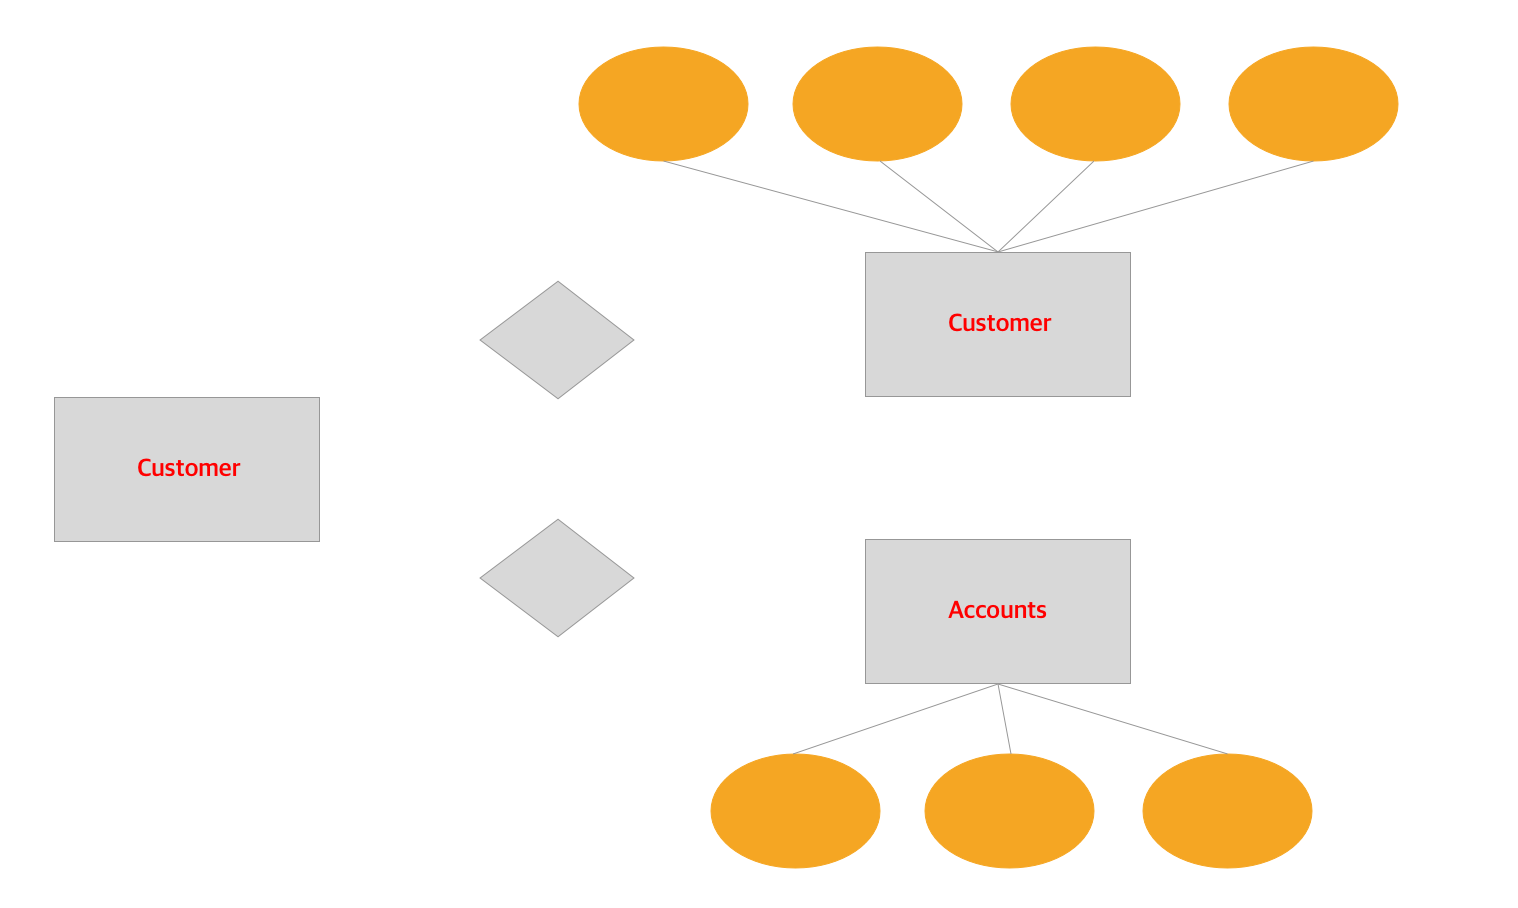
\includegraphics[width=\linewidth]{images/worksheet_14_solution_13.png}
    \end{center}

    \bigskip

    \begin{mdframed}
        \underline{\textbf{Correct Solution:}}

        \bigskip

        \begin{center}
        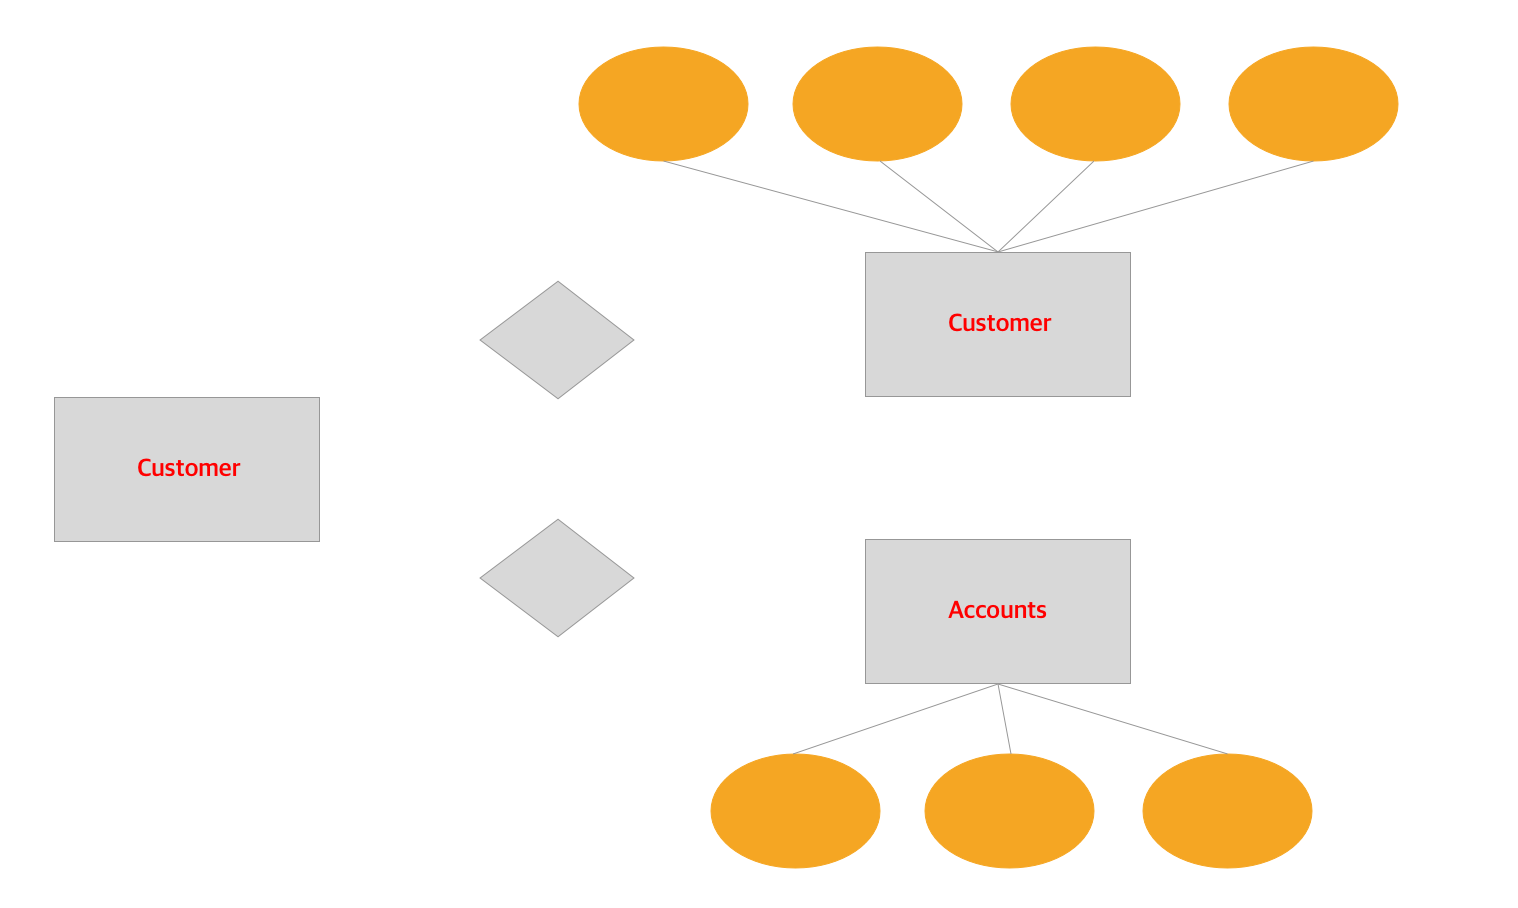
\includegraphics[width=\linewidth]{images/worksheet_14_solution_13.png}
        \end{center}

    \end{mdframed}

    \bigskip

    \underline{\textbf{Notes:}}

    \bigskip

    \begin{itemize}
        \item E/R Model
        \begin{itemize}
            \item Means \textbf{Entity Relationship Model}
            \item Entity Relationship Model(ER Modeling) is a graphical approach to database design.
            \item Is comparable to class diagram in UML
            \item Uses three principle element types:

            \begin{enumerate}[1.]
                \item Entity sets
                \begin{itemize}
                    \item Is an abstract object of some sort (i.e. entitiy)
                    \item Is not used to represent class
                    \item Is represented by rectangles
                \end{itemize}

                \begin{center}
                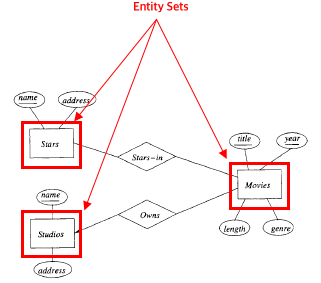
\includegraphics[width=0.7\linewidth]{images/worksheet_14_solution_1.png}
                \end{center}

                \item Attributes
                \begin{itemize}
                    \item Are properties of entities in a set (i.e. column name)
                    \item Each has its own primitive data types (e.g. String, integers, Reals)
                    \item Is represented by ovals
                \end{itemize}

                \begin{center}
                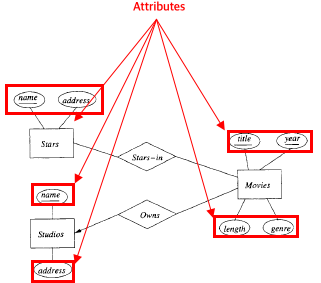
\includegraphics[width=0.7\linewidth]{images/worksheet_14_solution_2.png}
                \end{center}

                \item Relationships
                \begin{itemize}
                    \item Are connections among two or more entity sets (e.g. intermediary Relations like Stars In)
                    \item Is represented by diamond
                \end{itemize}

                \begin{center}
                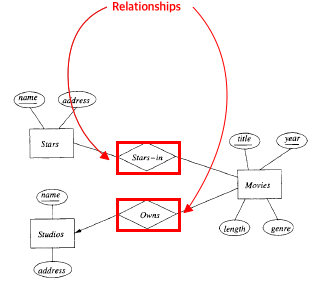
\includegraphics[width=0.7\linewidth]{images/worksheet_14_solution_3.png}
                \end{center}
            \end{enumerate}

            \bigskip

            \underline{\textbf{Example:}}

            \bigskip

            \begin{center}
            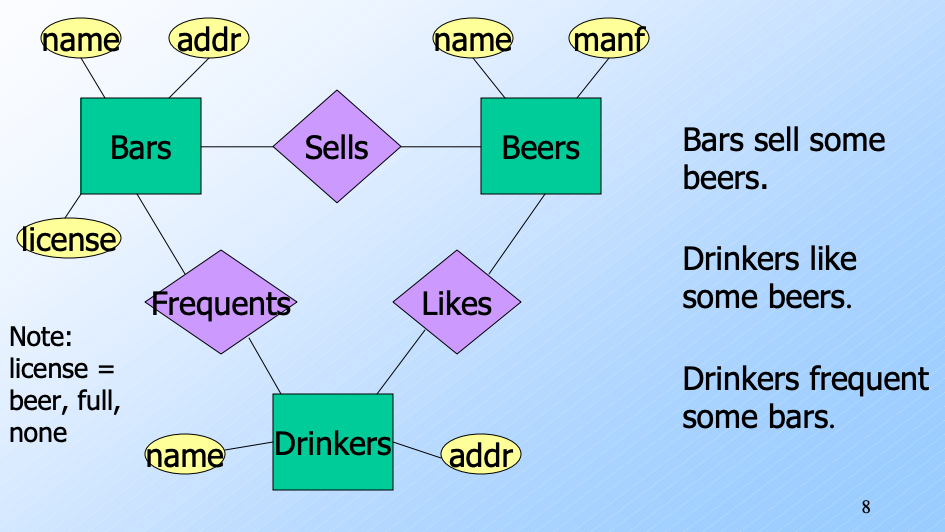
\includegraphics[width=0.7\linewidth]{images/worksheet_14_solution_4.png}
            \end{center}
        \end{itemize}

        \item Multiway Relationships

        \begin{itemize}
            \item Connects more than two relationship sets
            \item Enables to represent relationships that otherwise is
            difficult in binary relationship
            \item Arrow $\to$ 'one'
            \item No arrow $\to$ 'many'
        \end{itemize}

        \bigskip

        \underline{\textbf{Example:}}

        \bigskip

        \begin{center}
        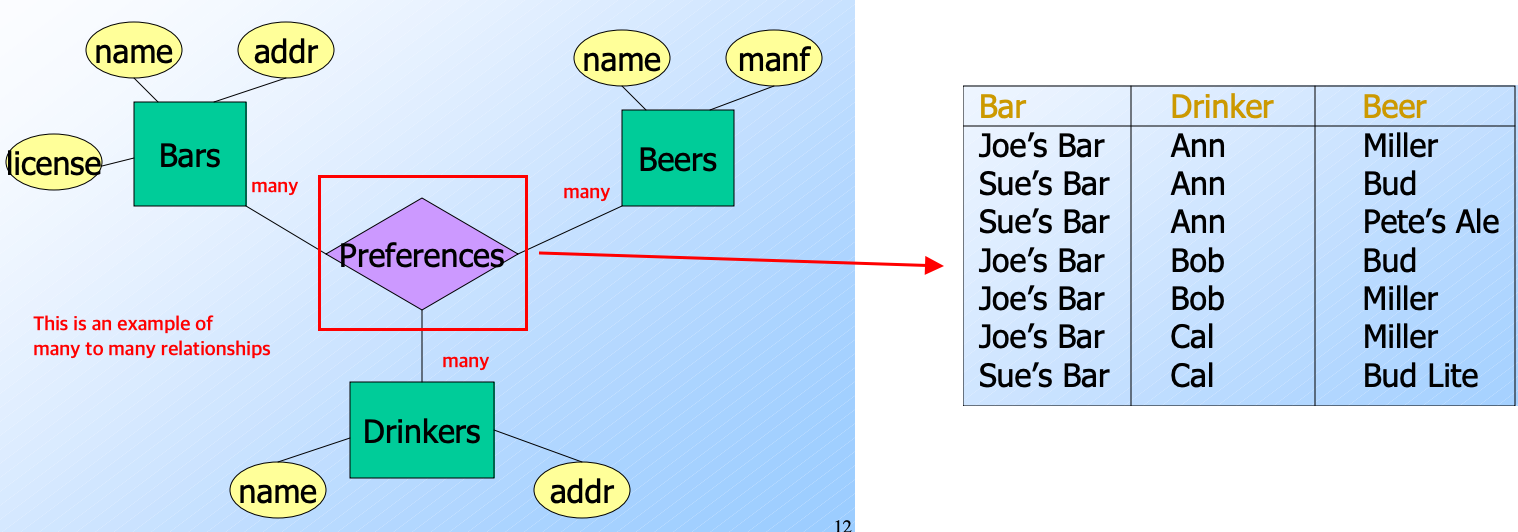
\includegraphics[width=\linewidth]{images/worksheet_14_solution_5.png}
        \end{center}

        \bigskip

        \underline{\textbf{Example 2:}}

        \bigskip

        \begin{center}
        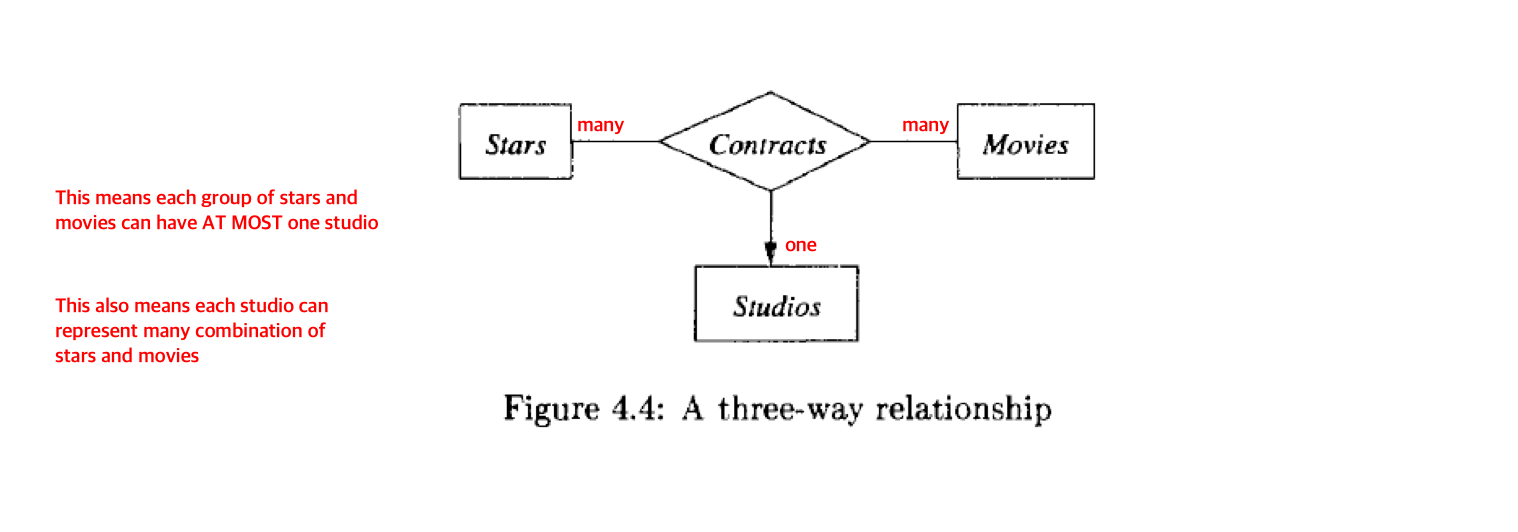
\includegraphics[width=\linewidth]{images/worksheet_14_solution_6.png}
        \end{center}

        \bigskip

        \item Roles in Relationships
        \begin{itemize}
            \item Is the label of edges between the entity set and relationship
            \item Are used to clarify the sementics of relationship
        \end{itemize}

        \bigskip

        \underline{\textbf{Example:}}

        \bigskip

        \begin{center}
        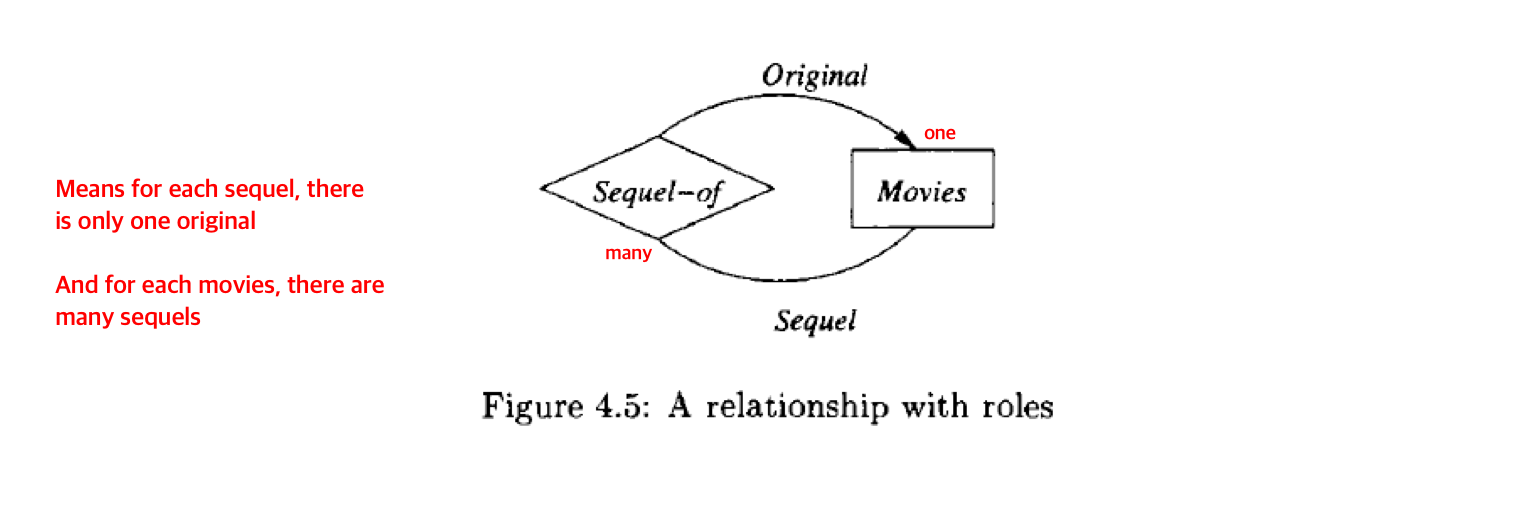
\includegraphics[width=\linewidth]{images/worksheet_14_solution_7.png}
        \end{center}

        \bigskip

        \underline{\textbf{Example 2:}}

        \bigskip

        \begin{center}
        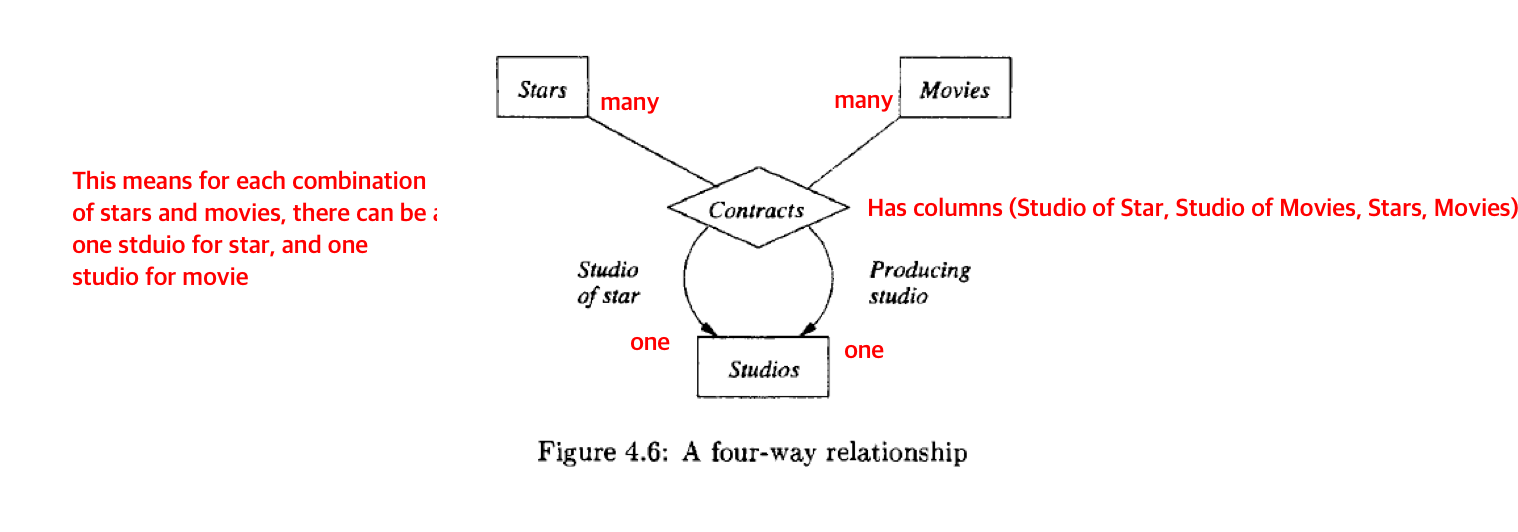
\includegraphics[width=\linewidth]{images/worksheet_14_solution_8.png}
        \end{center}

        \item Attributes on Relationships

        \begin{itemize}
            \item can be thought as a property of tuples in the relationship set
            (i.e. String, Integer, Float, Boolean)

            \bigskip

            \underline{\textbf{Example:}}

            \bigskip

            \begin{center}
            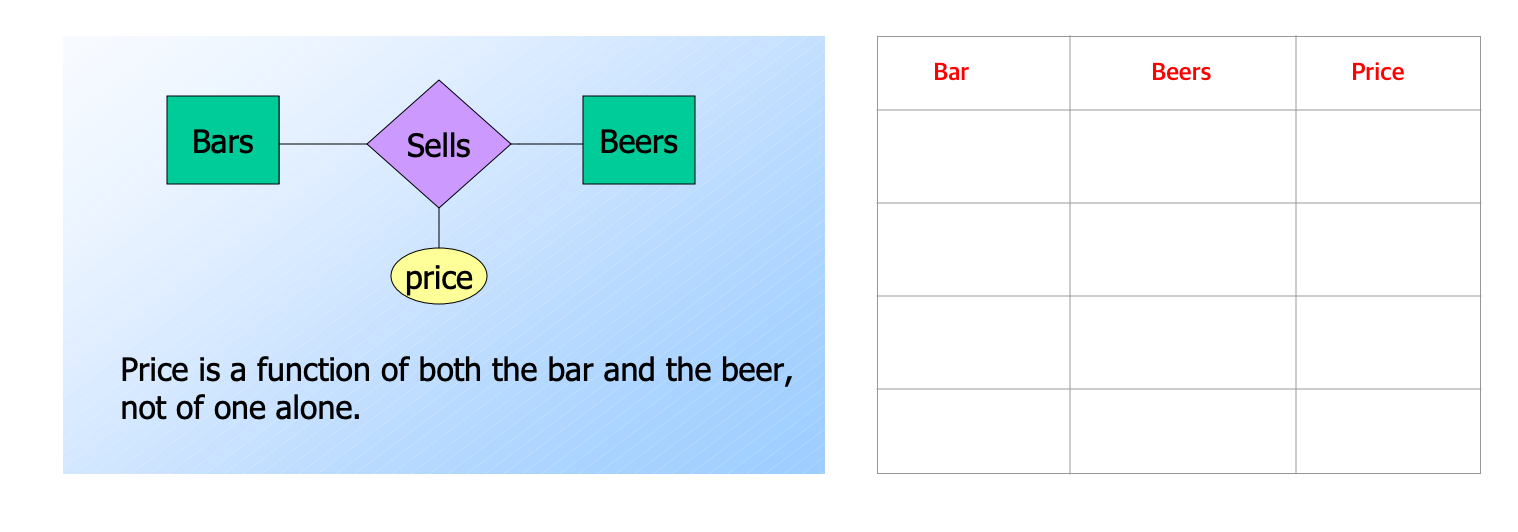
\includegraphics[width=\linewidth]{images/worksheet_14_solution_9.png}
            \end{center}

            \item Can be removed by creating an entity set with the attribute

            \bigskip

              \underline{\textbf{Example:}}

            \bigskip

            \begin{center}
            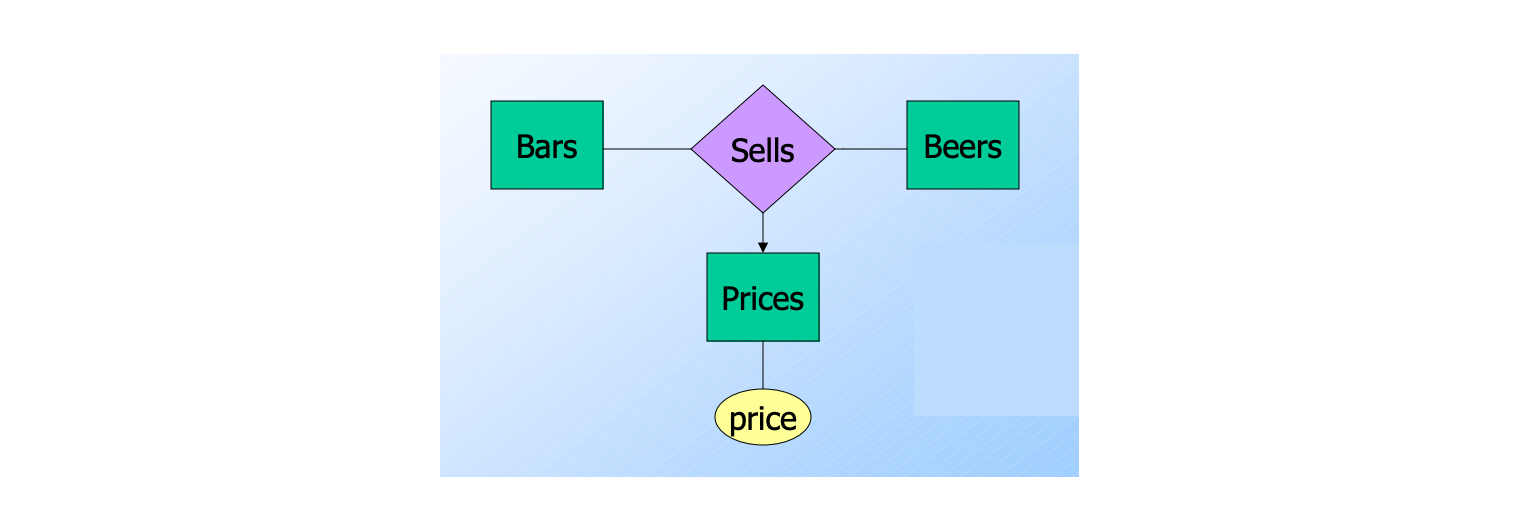
\includegraphics[width=\linewidth]{images/worksheet_14_solution_10.png}
            \end{center}
        \end{itemize}

        \item Conversting Multiway Relationships to Binary

        \bigskip

        \underline{\textbf{Example:}}

        \bigskip

        \begin{center}
        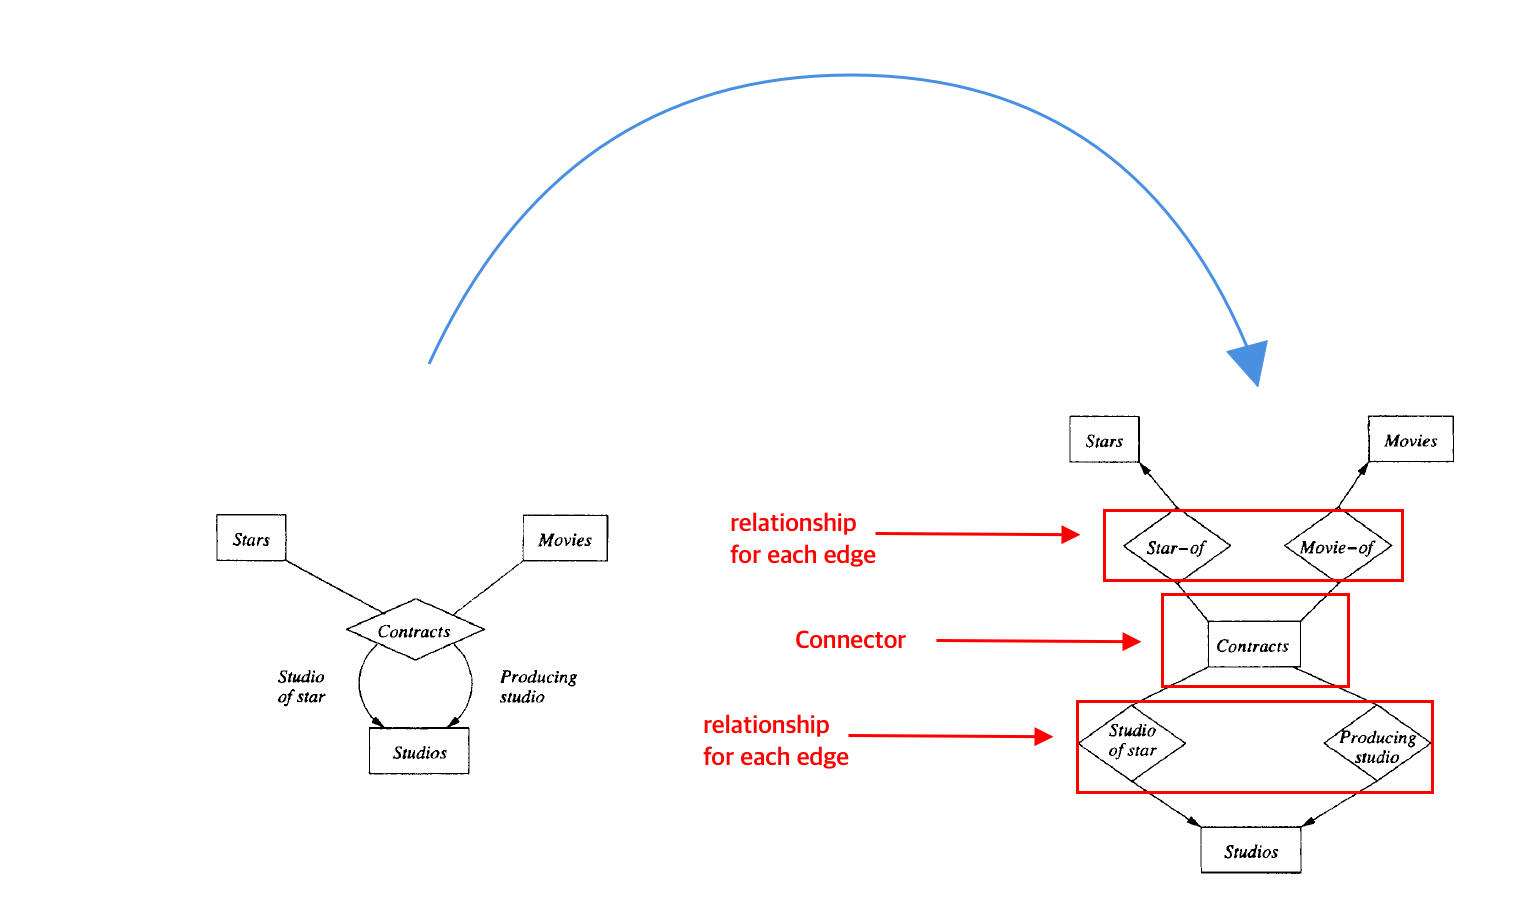
\includegraphics[width=\linewidth]{images/worksheet_14_solution_11.png}
        \end{center}


        \item Subclasses in the E/R Model

        \begin{itemize}
            \item Has its own special attributes and/or relationships
            \item All `\textit{isa}' relationship is \underline{one to one}
            \item Is represented by triangle with label `\textit{isa}' followed by
            entity set
        \end{itemize}

        \bigskip

        \underline{\textbf{Example:}}

        \bigskip

        \begin{center}
        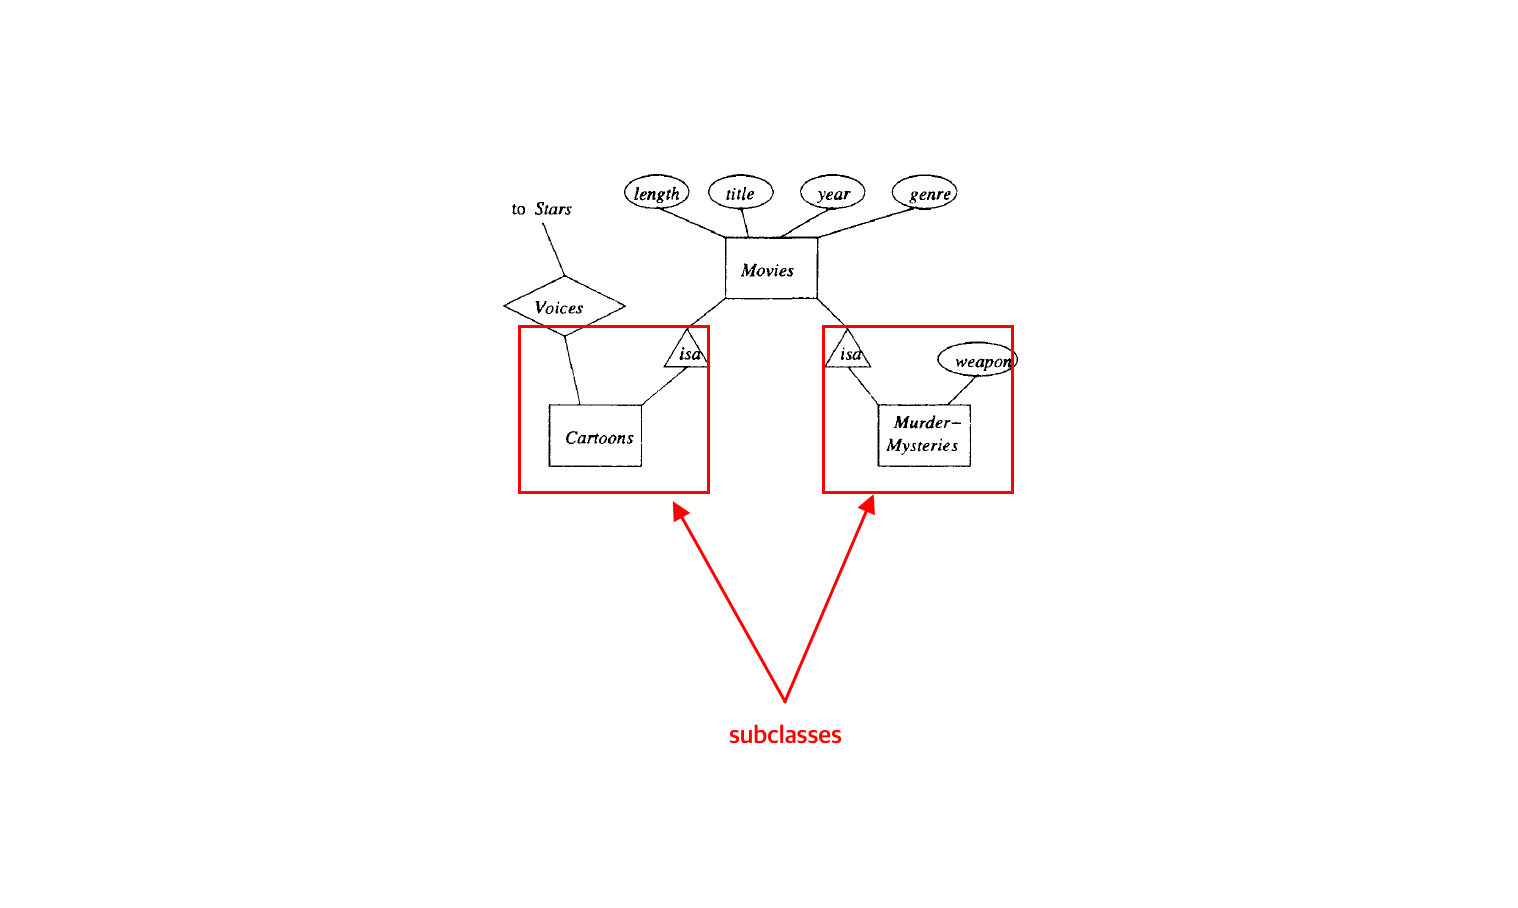
\includegraphics[width=\linewidth]{images/worksheet_14_solution_12.png}
        \end{center}

        \bigskip



    \end{itemize}

    \item

    \begin{enumerate}[a)]
        \item

        \begin{center}
        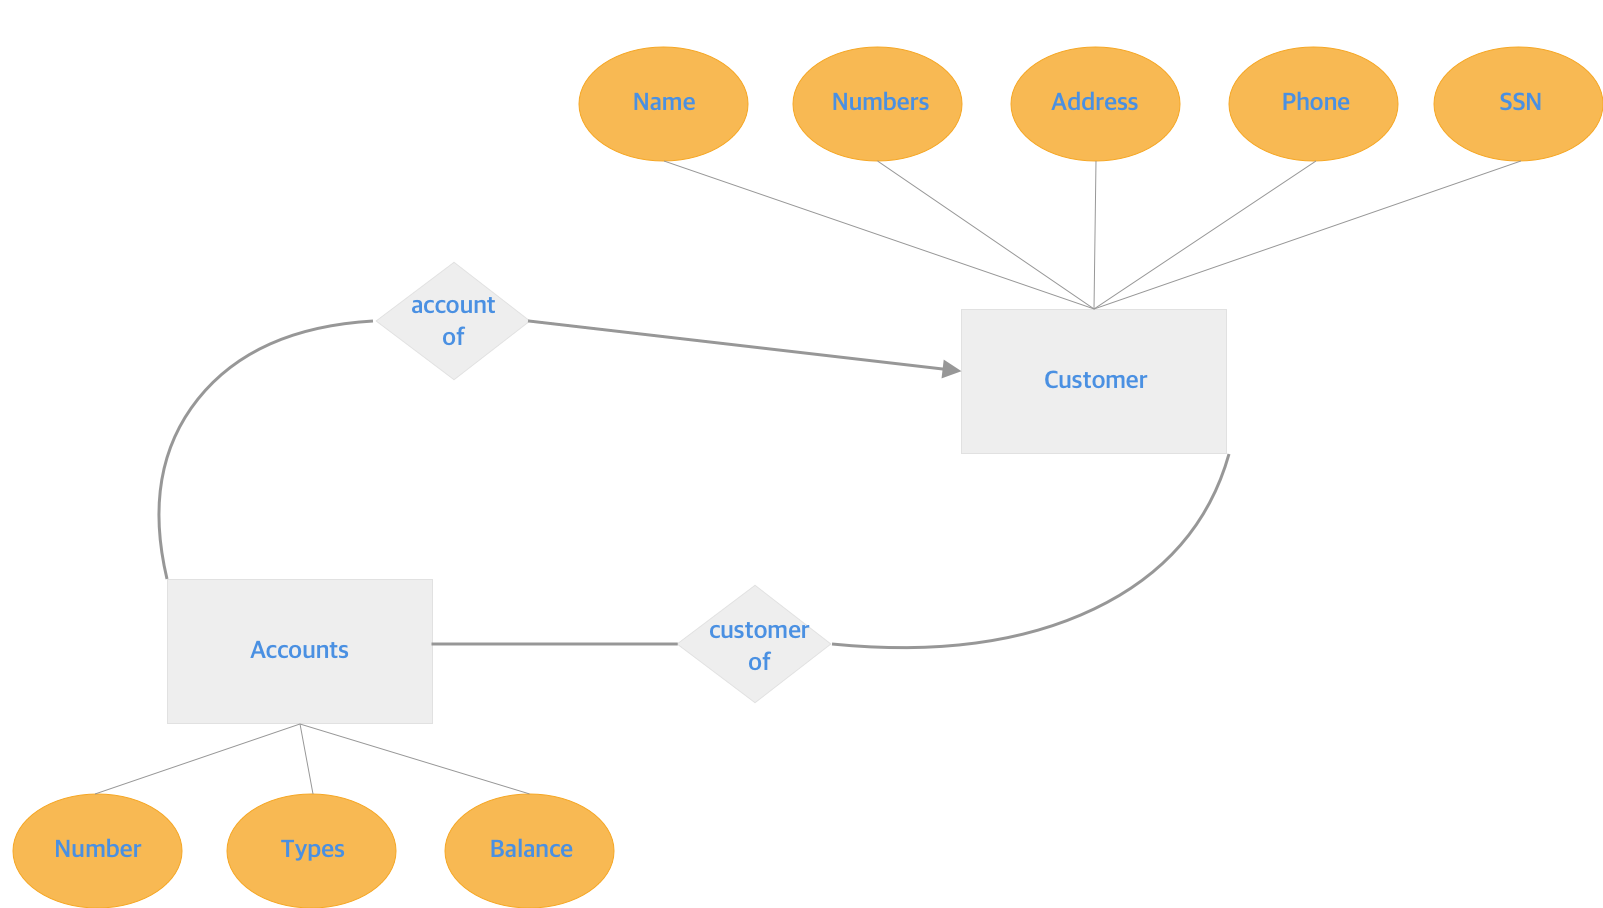
\includegraphics[width=\linewidth]{images/worksheet_14_solution_15.png}
        \end{center}

        \bigskip

        \begin{mdframed}
            \underline{\textbf{Correct Solution:}}

            \bigskip

            \begin{center}
            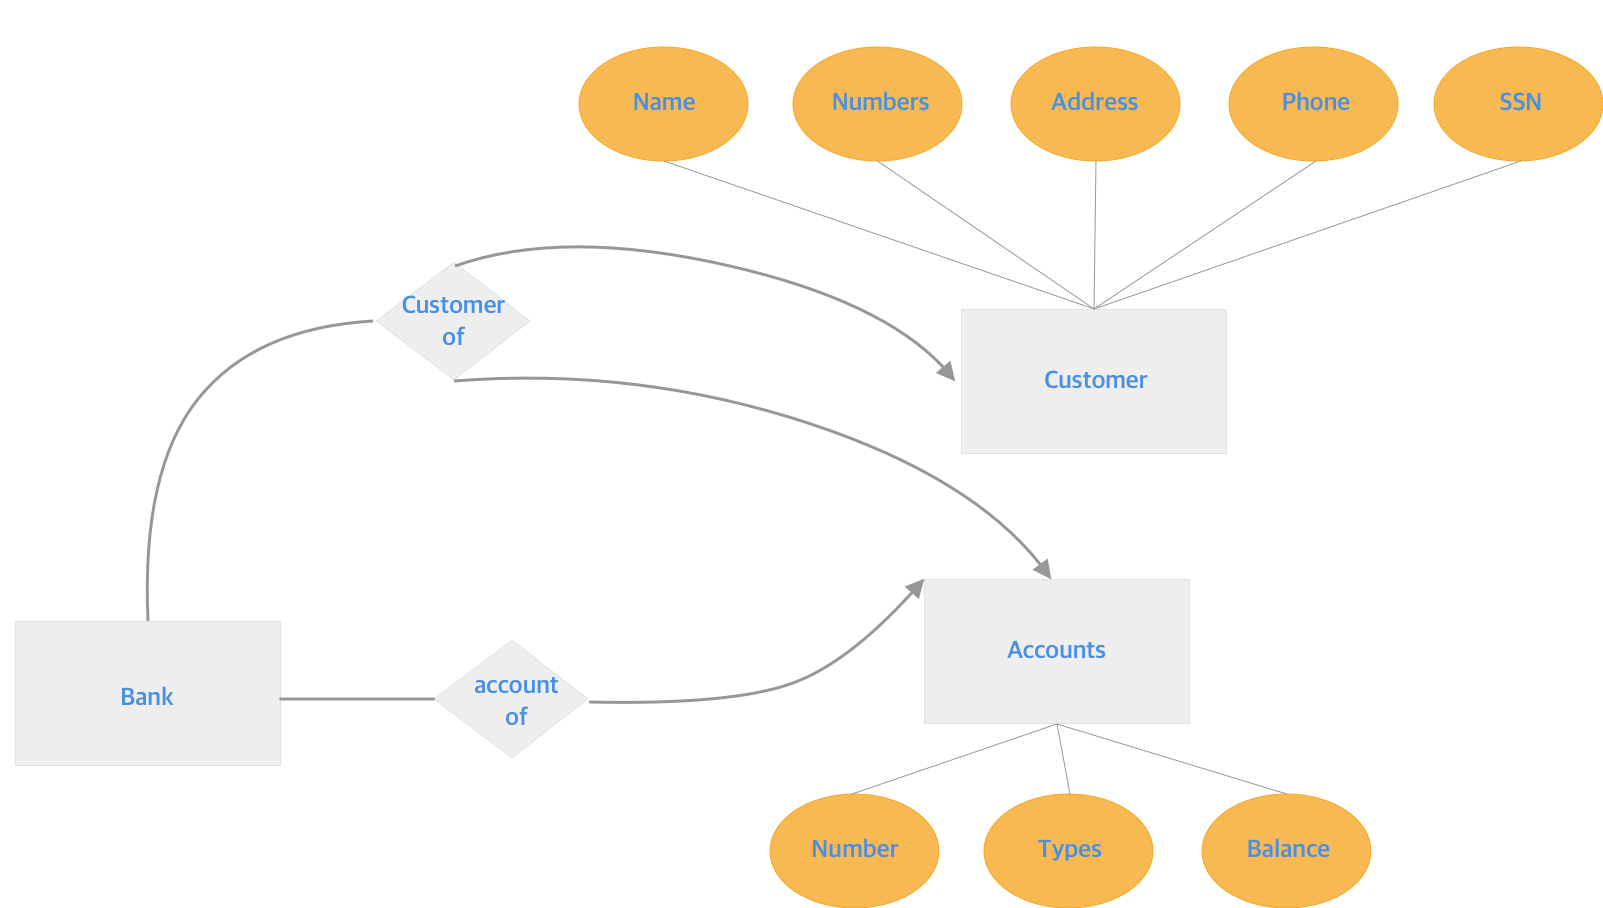
\includegraphics[width=\linewidth]{images/worksheet_14_solution_17.png}
            \end{center}
        \end{mdframed}

        \item

        \begin{center}
        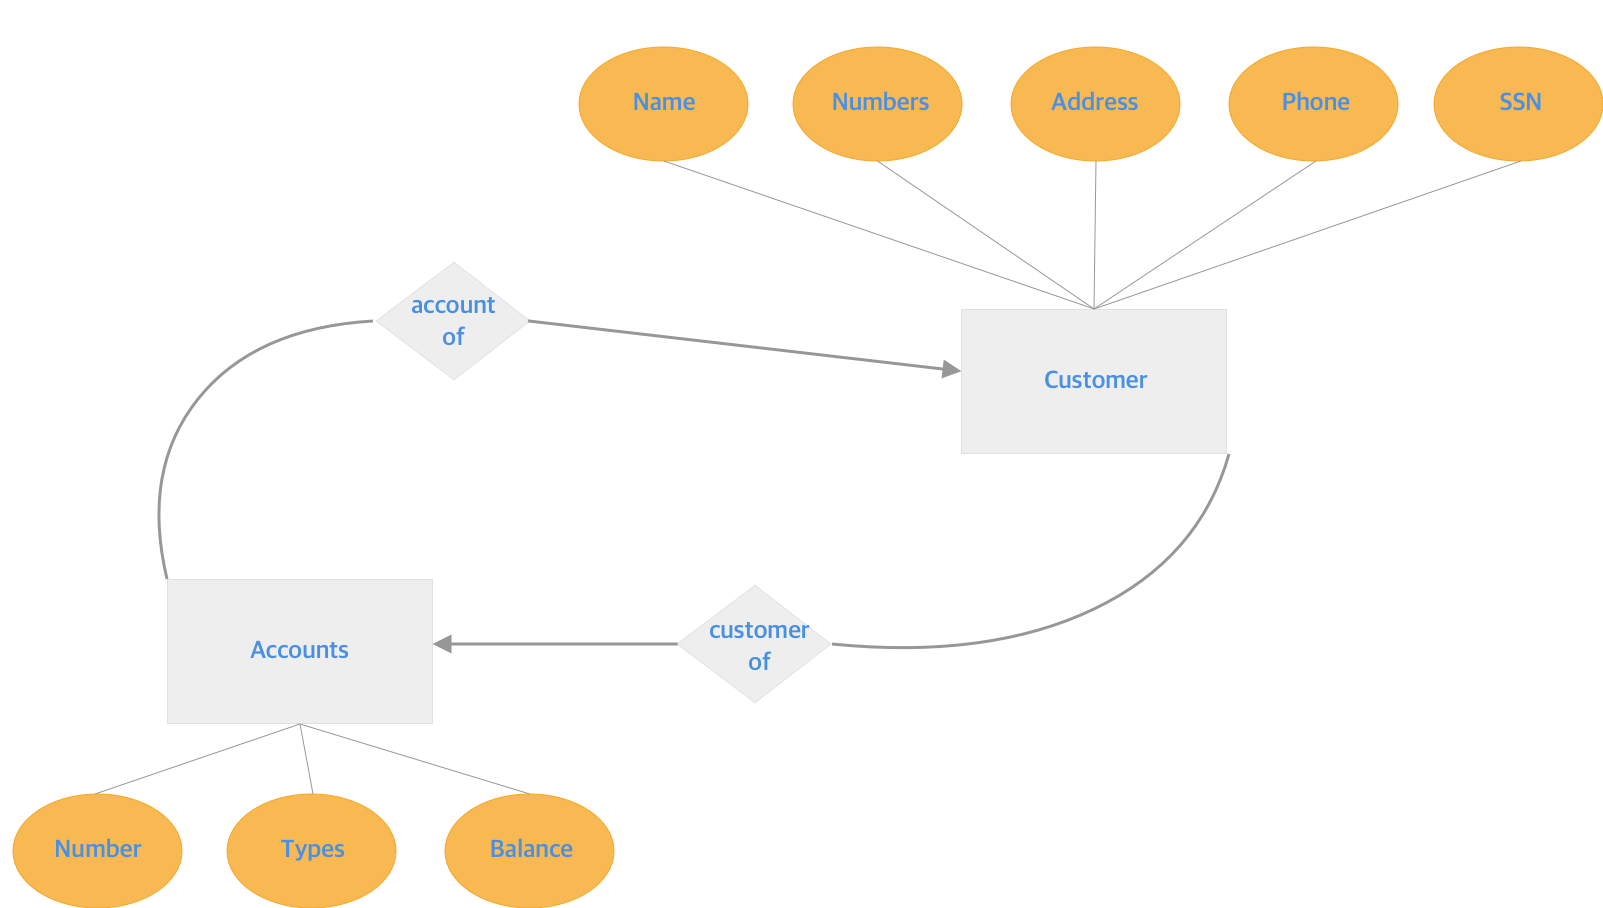
\includegraphics[width=\linewidth]{images/worksheet_14_solution_16.png}
        \end{center}

        \bigskip

        \begin{mdframed}
            \underline{\textbf{Correct Solution:}}

            \bigskip

            \begin{center}
            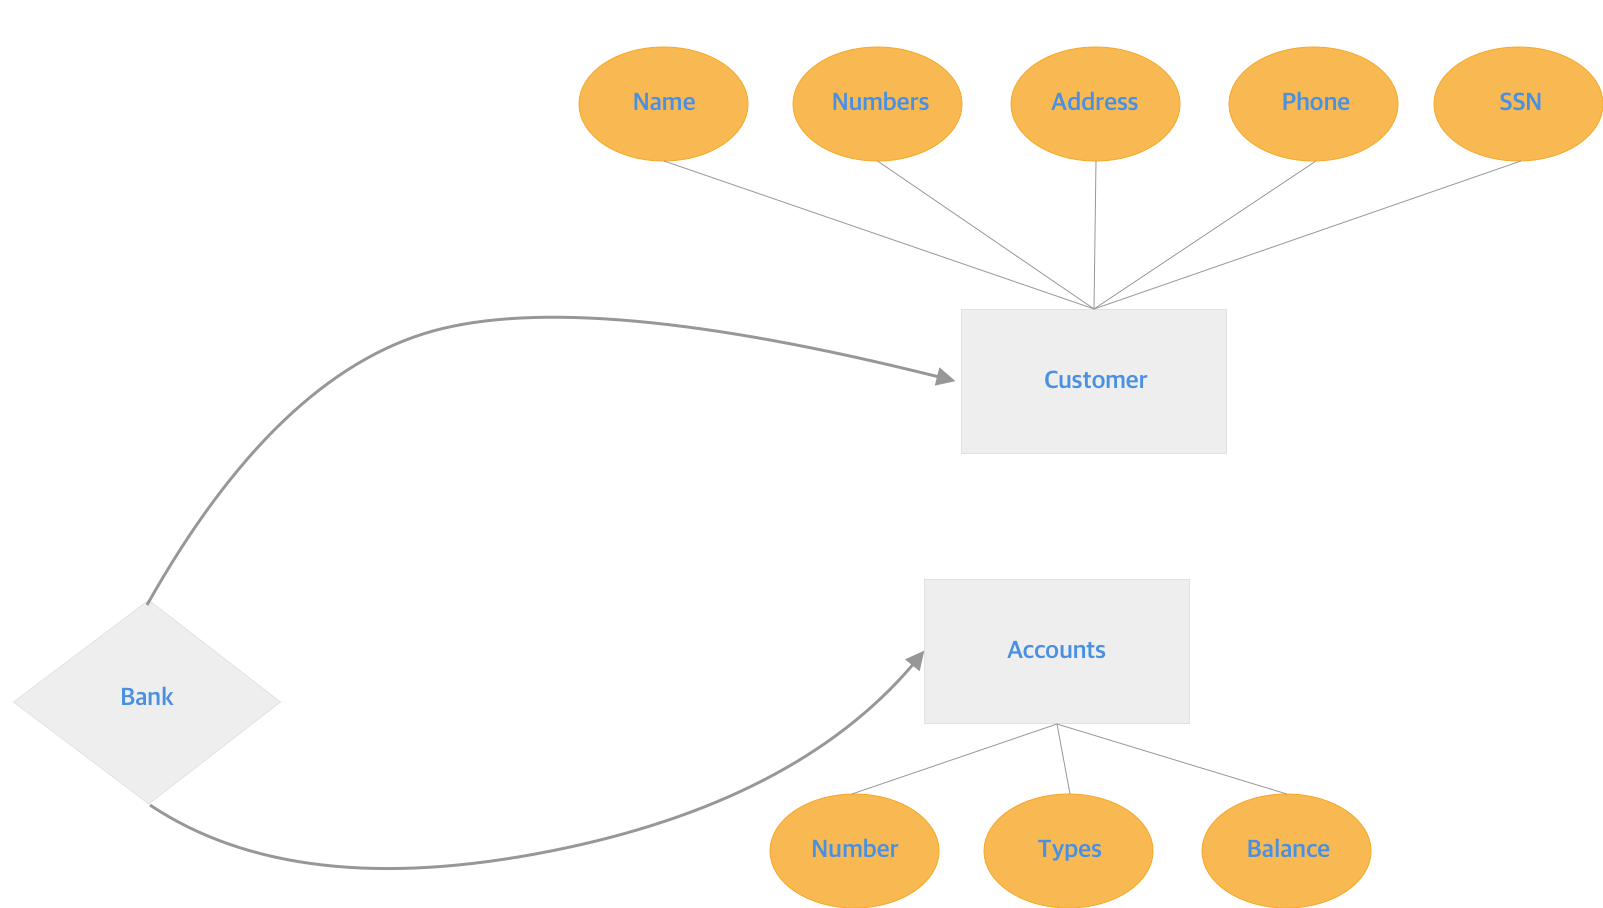
\includegraphics[width=\linewidth]{images/worksheet_14_solution_18.png}
            \end{center}
        \end{mdframed}

        \item

        \begin{center}
        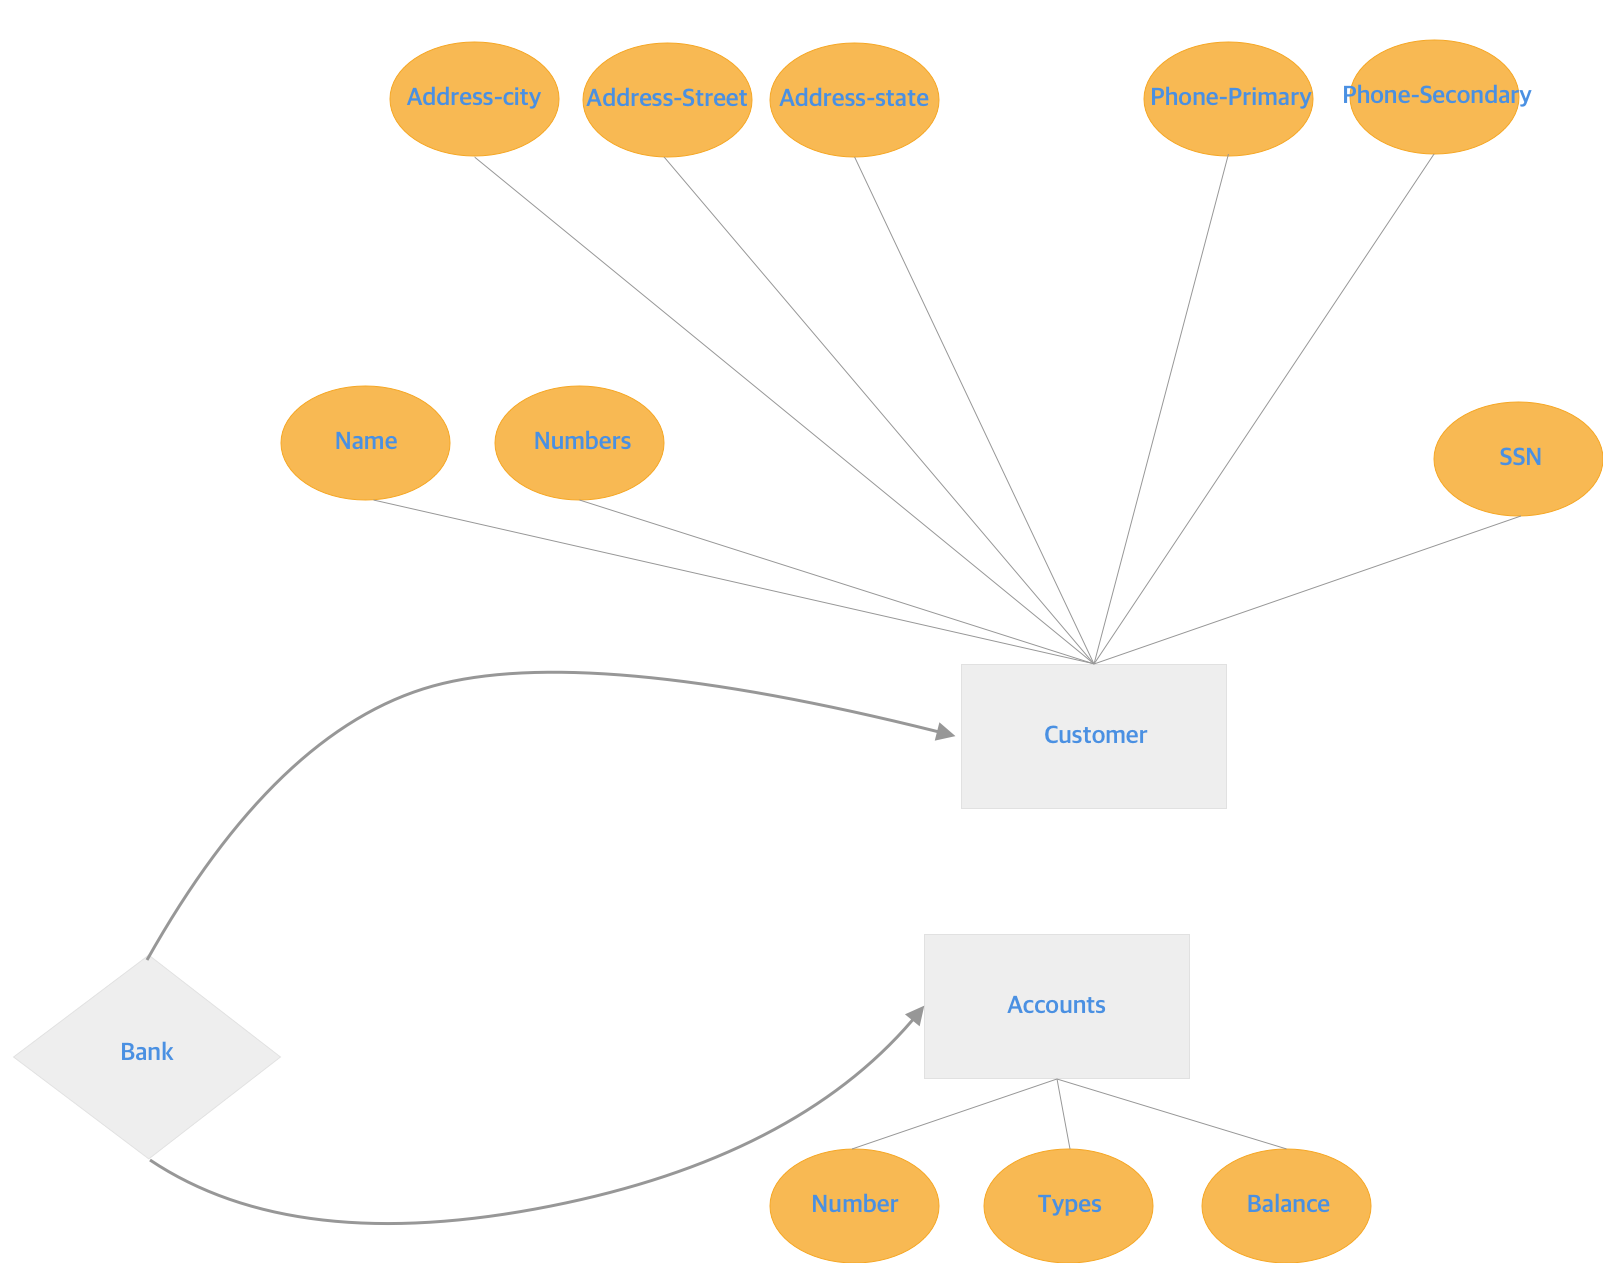
\includegraphics[width=\linewidth]{images/worksheet_14_solution_19.png}
        \end{center}

        \bigskip

        \begin{mdframed}
            \underline{\textbf{Correct Solution:}}

            \bigskip

            \begin{center}
            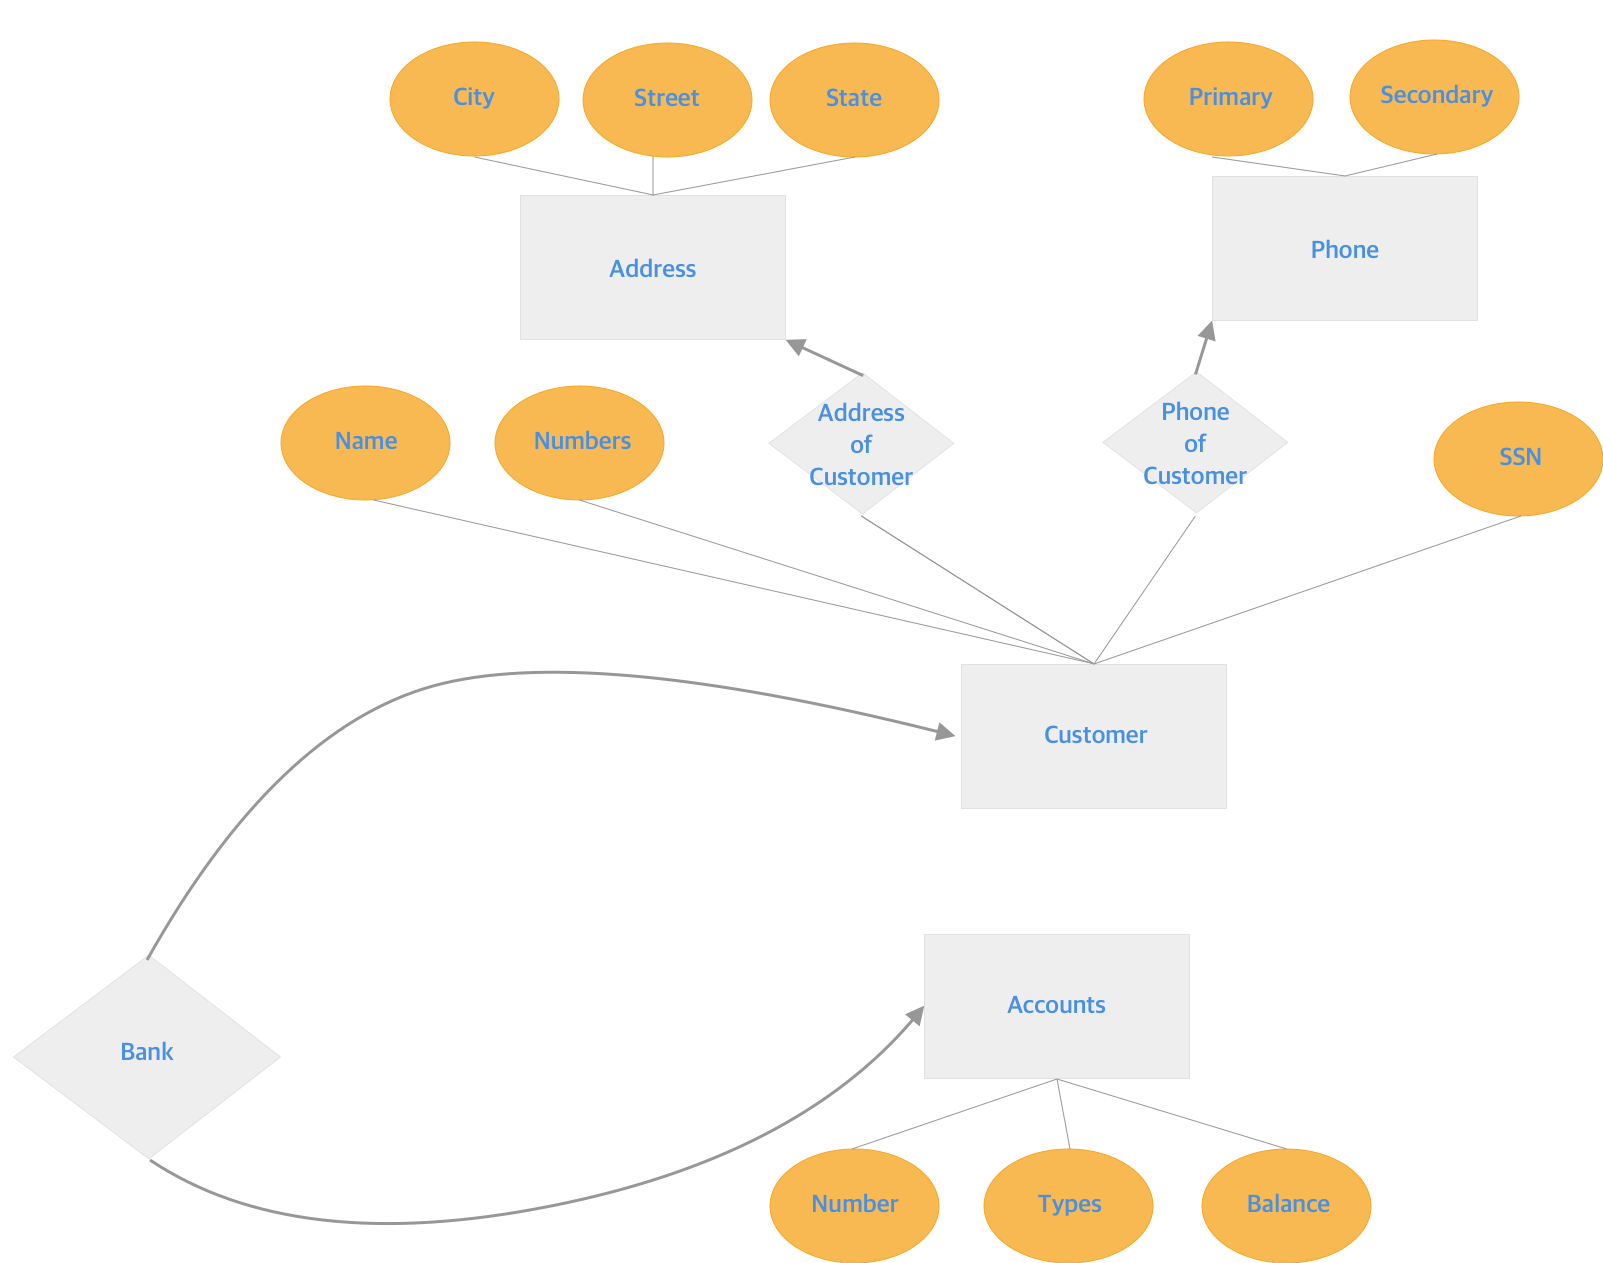
\includegraphics[width=\linewidth]{images/worksheet_14_solution_20.png}
            \end{center}

        \end{mdframed}

        \item

        \begin{center}
        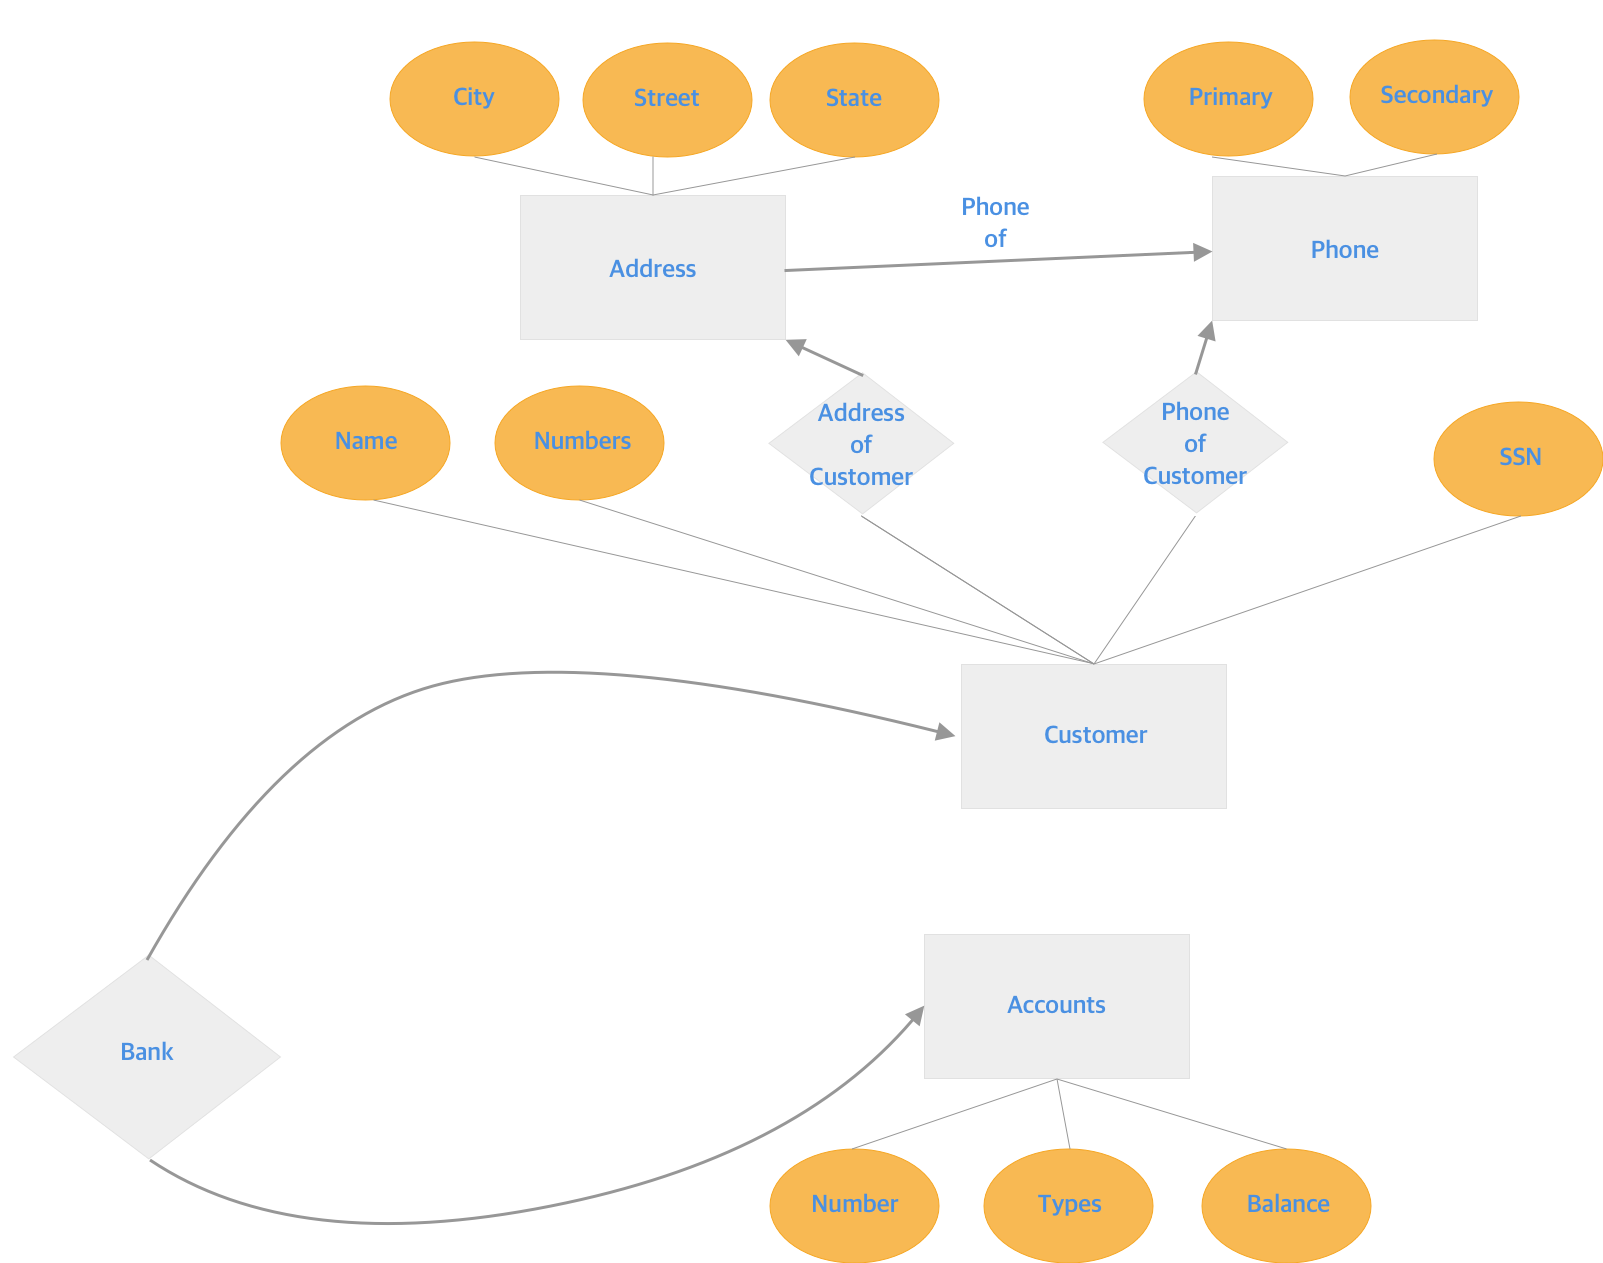
\includegraphics[width=\linewidth]{images/worksheet_14_solution_21.png}
        \end{center}

        \bigskip

        \begin{mdframed}
            \underline{\textbf{Correct Solution:}}

            \bigskip

            \begin{center}
            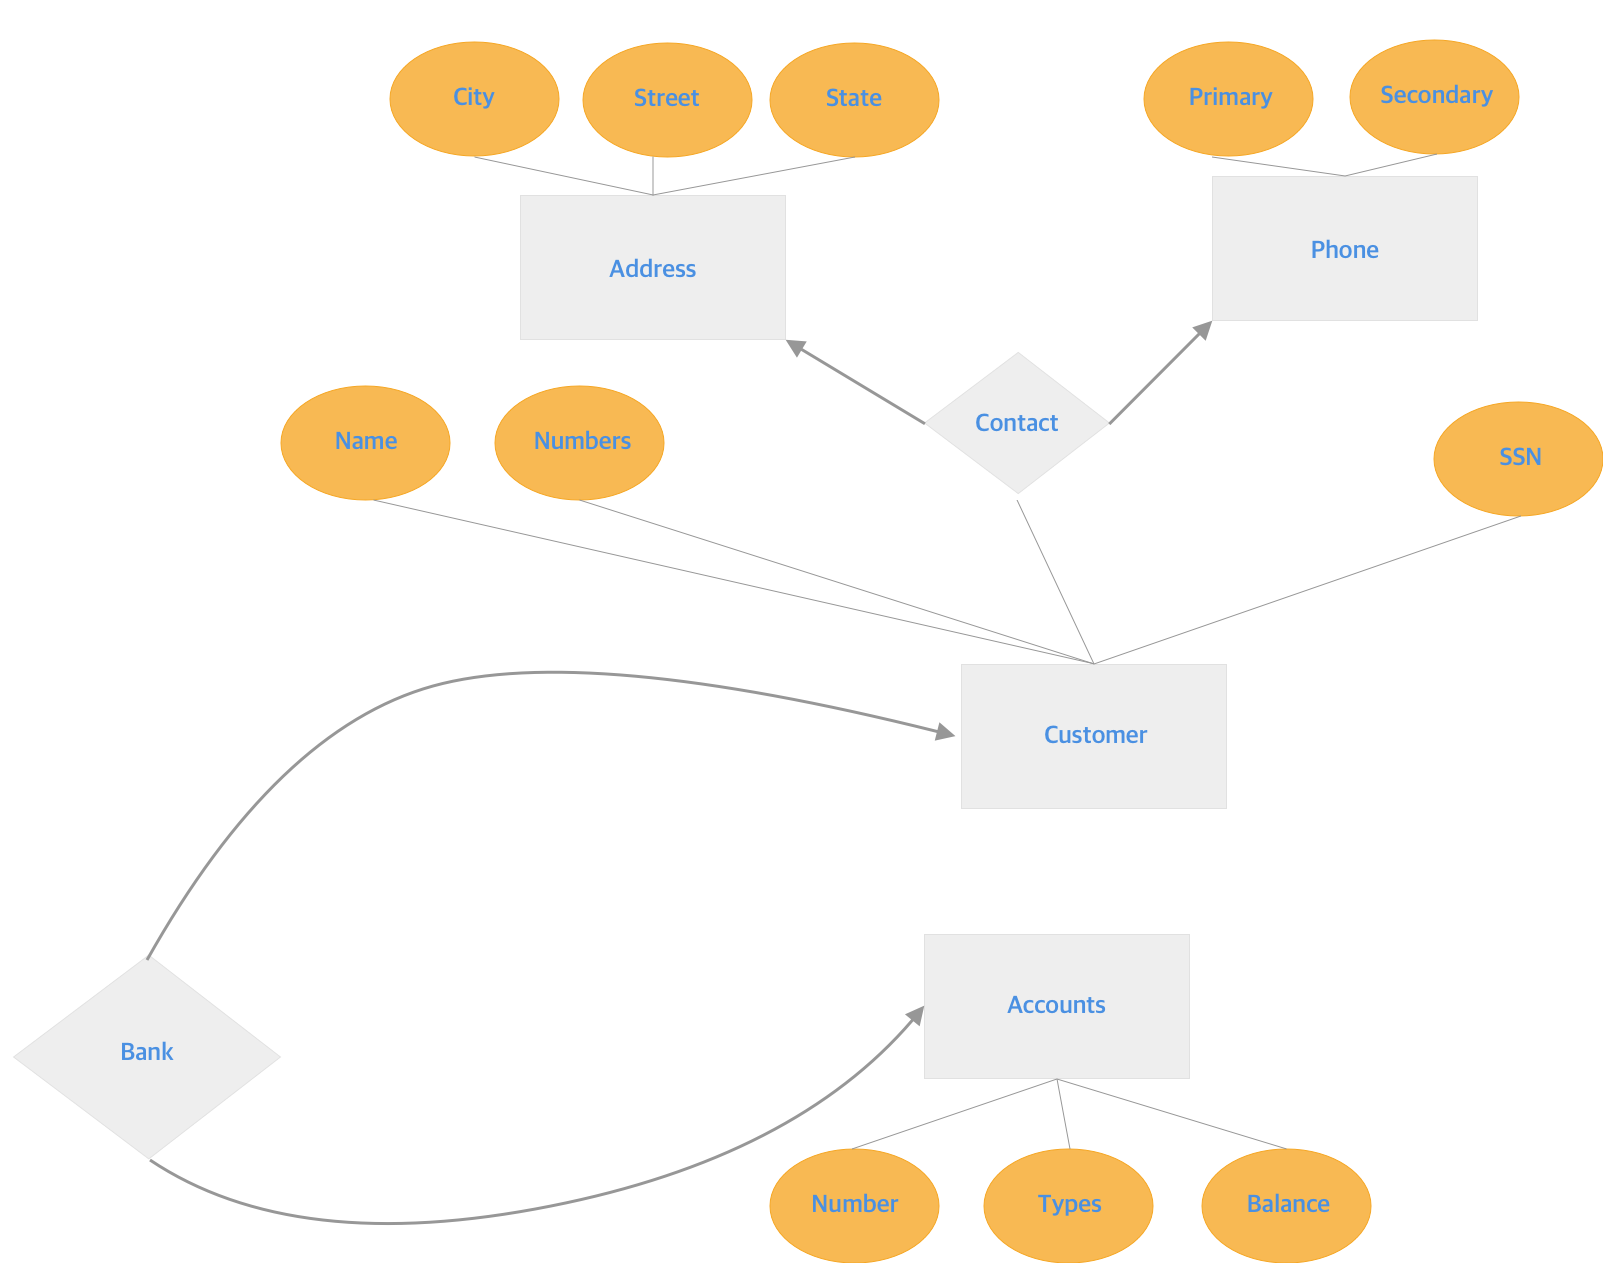
\includegraphics[width=\linewidth]{images/worksheet_14_solution_22.png}
            \end{center}

        \end{mdframed}

    \end{enumerate}

    \item

    \begin{center}
    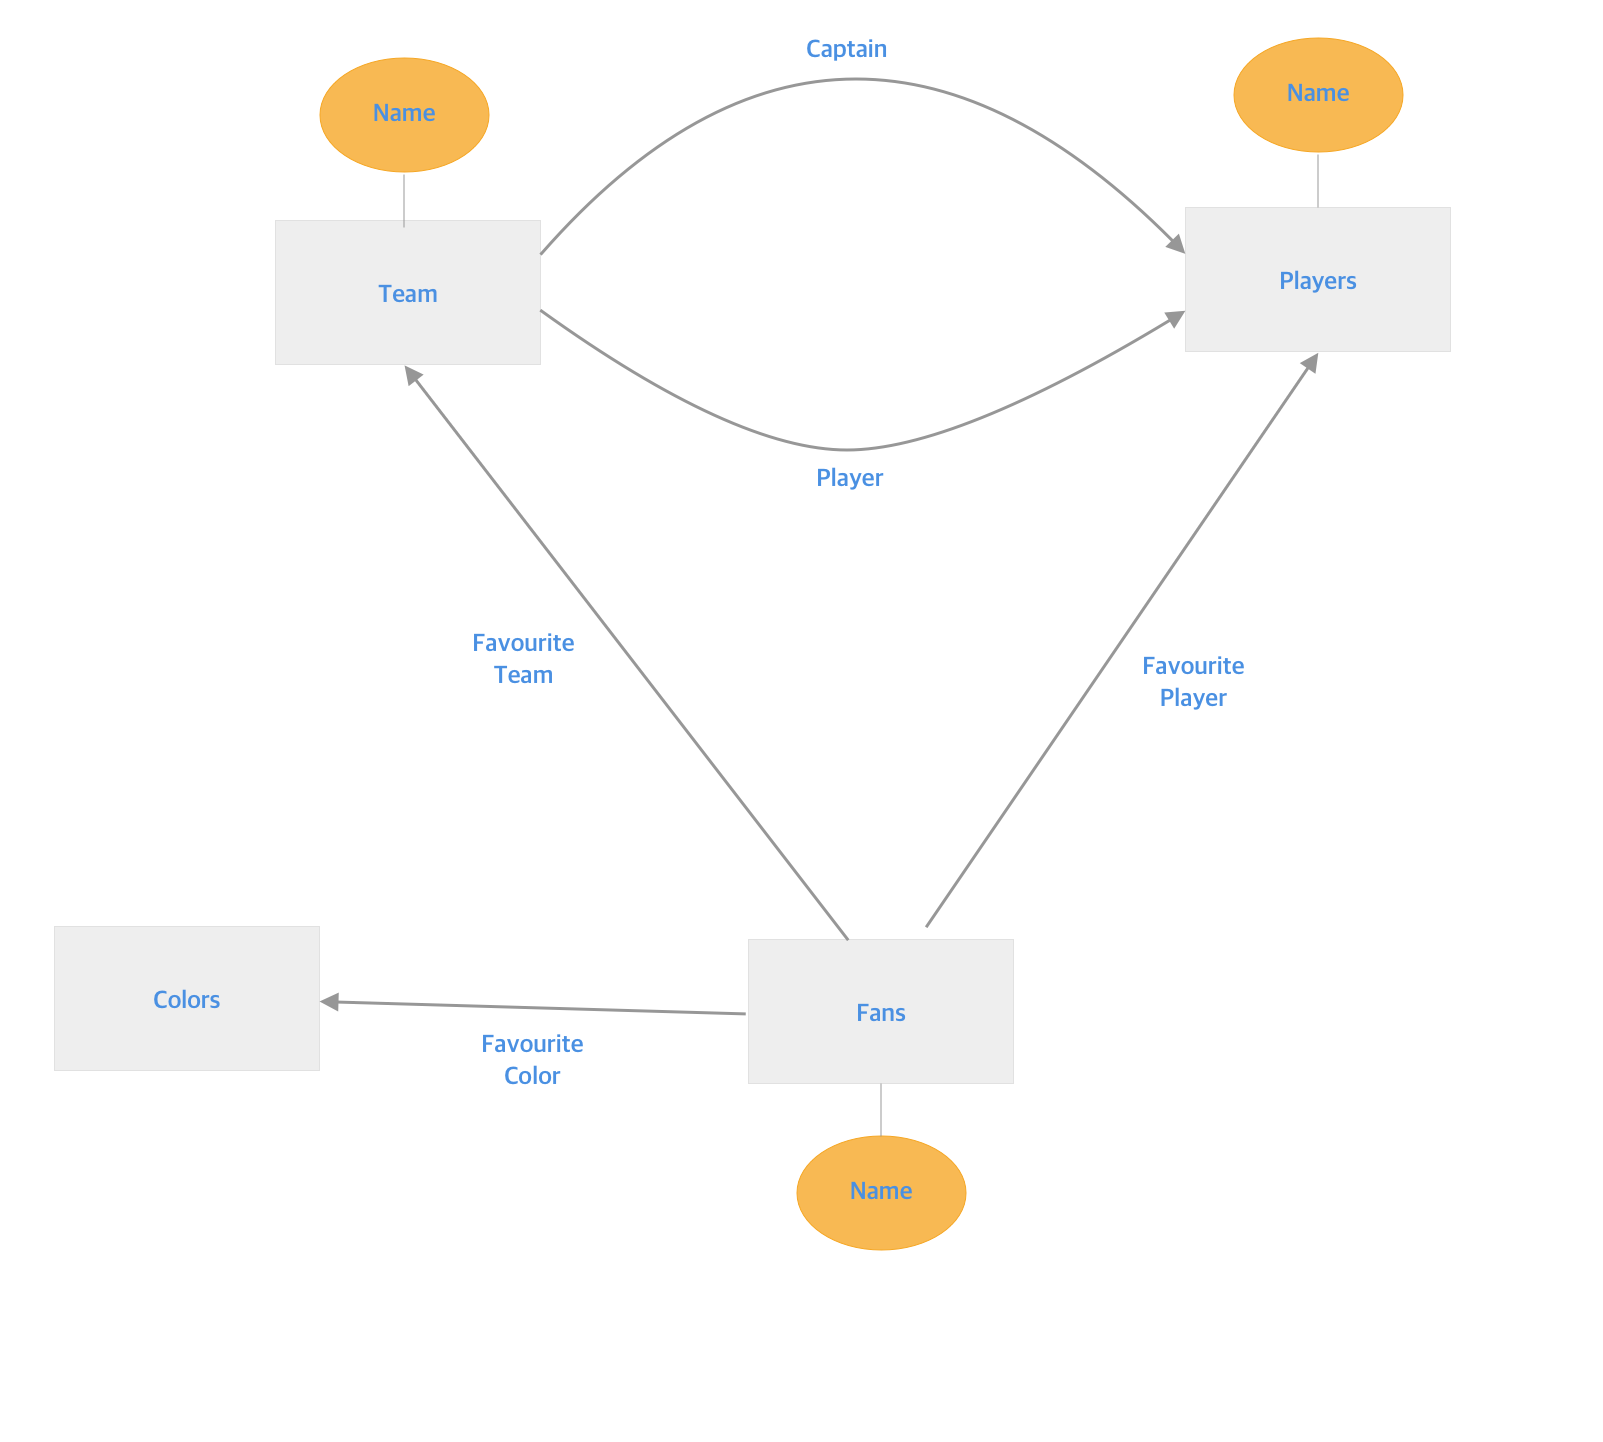
\includegraphics[width=\linewidth]{images/worksheet_14_solution_23.png}
    \end{center}

    \bigskip

    \begin{mdframed}

        \underline{\textbf{Correct Solution}}

        \bigskip

        \begin{center}
        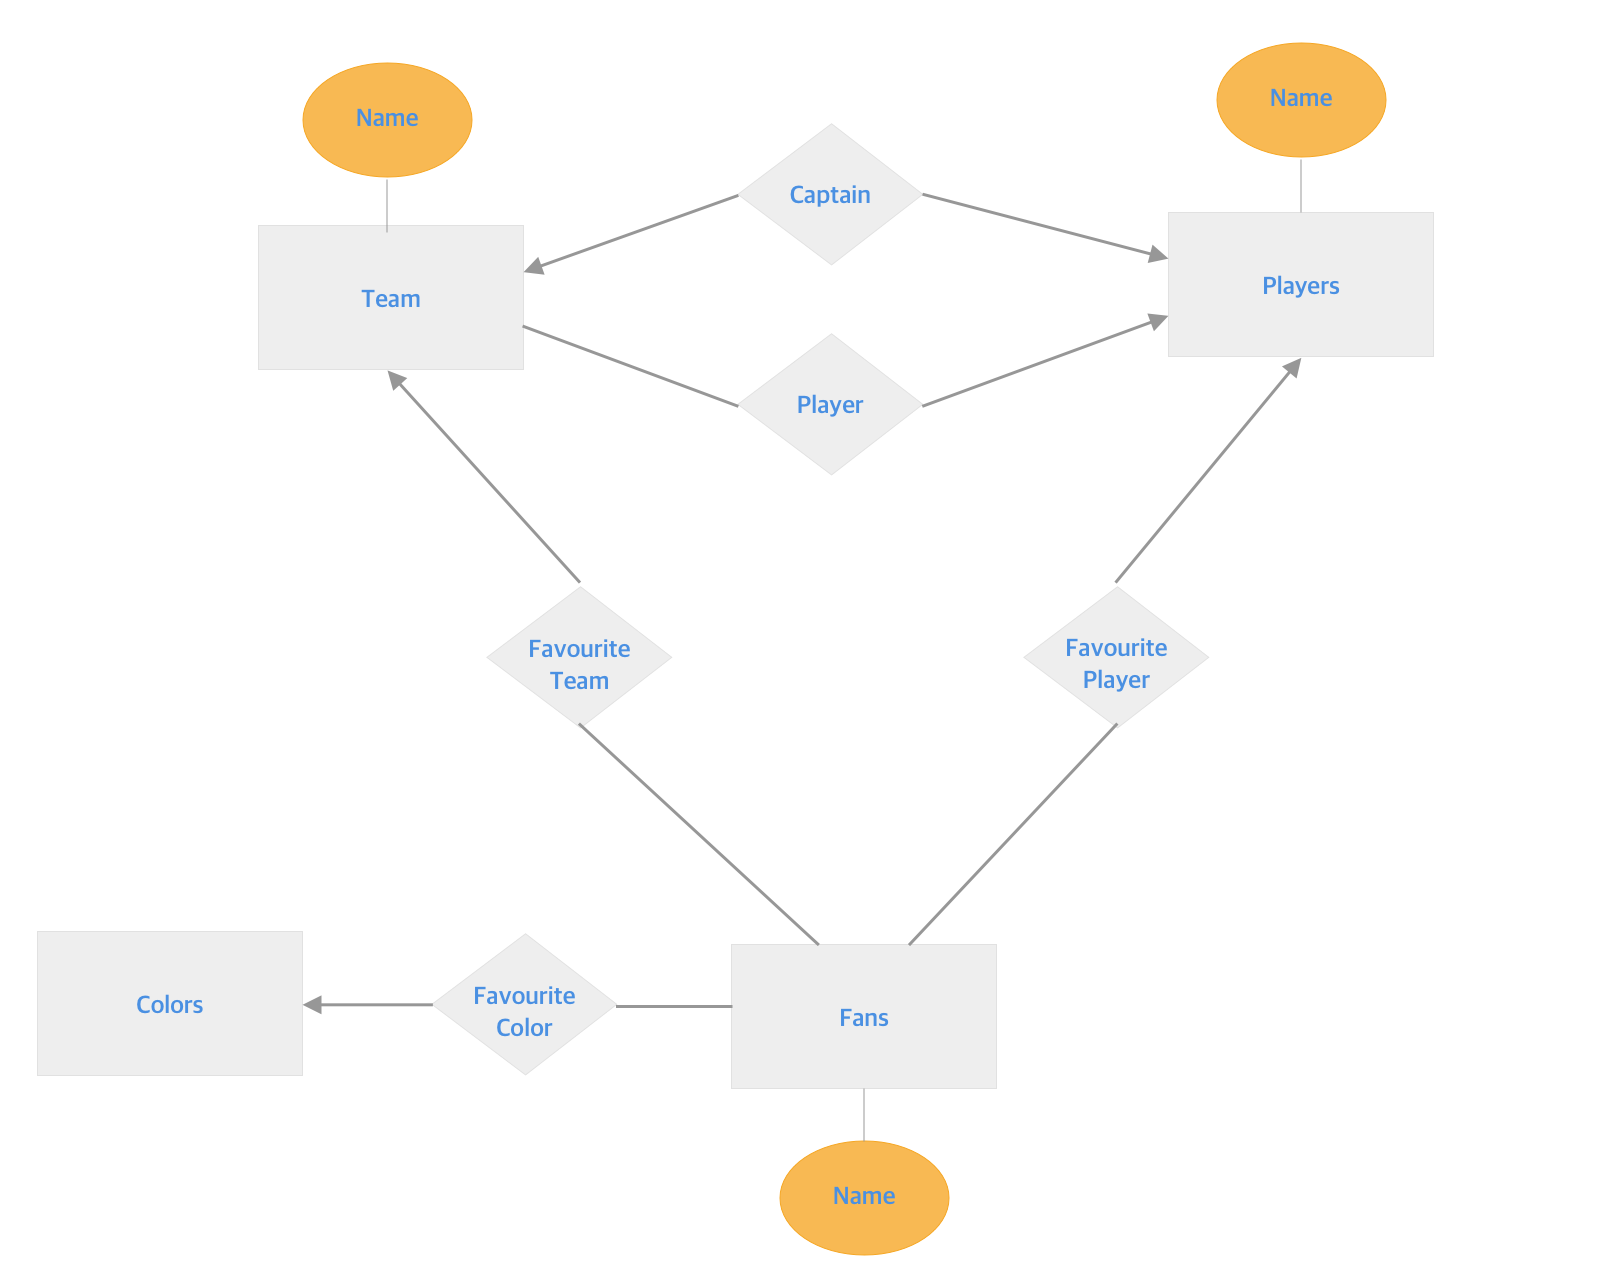
\includegraphics[width=\linewidth]{images/worksheet_14_solution_24.png}
        \end{center}

    \end{mdframed}

    \item


    \begin{enumerate}[a)]
        \item

        \begin{center}
        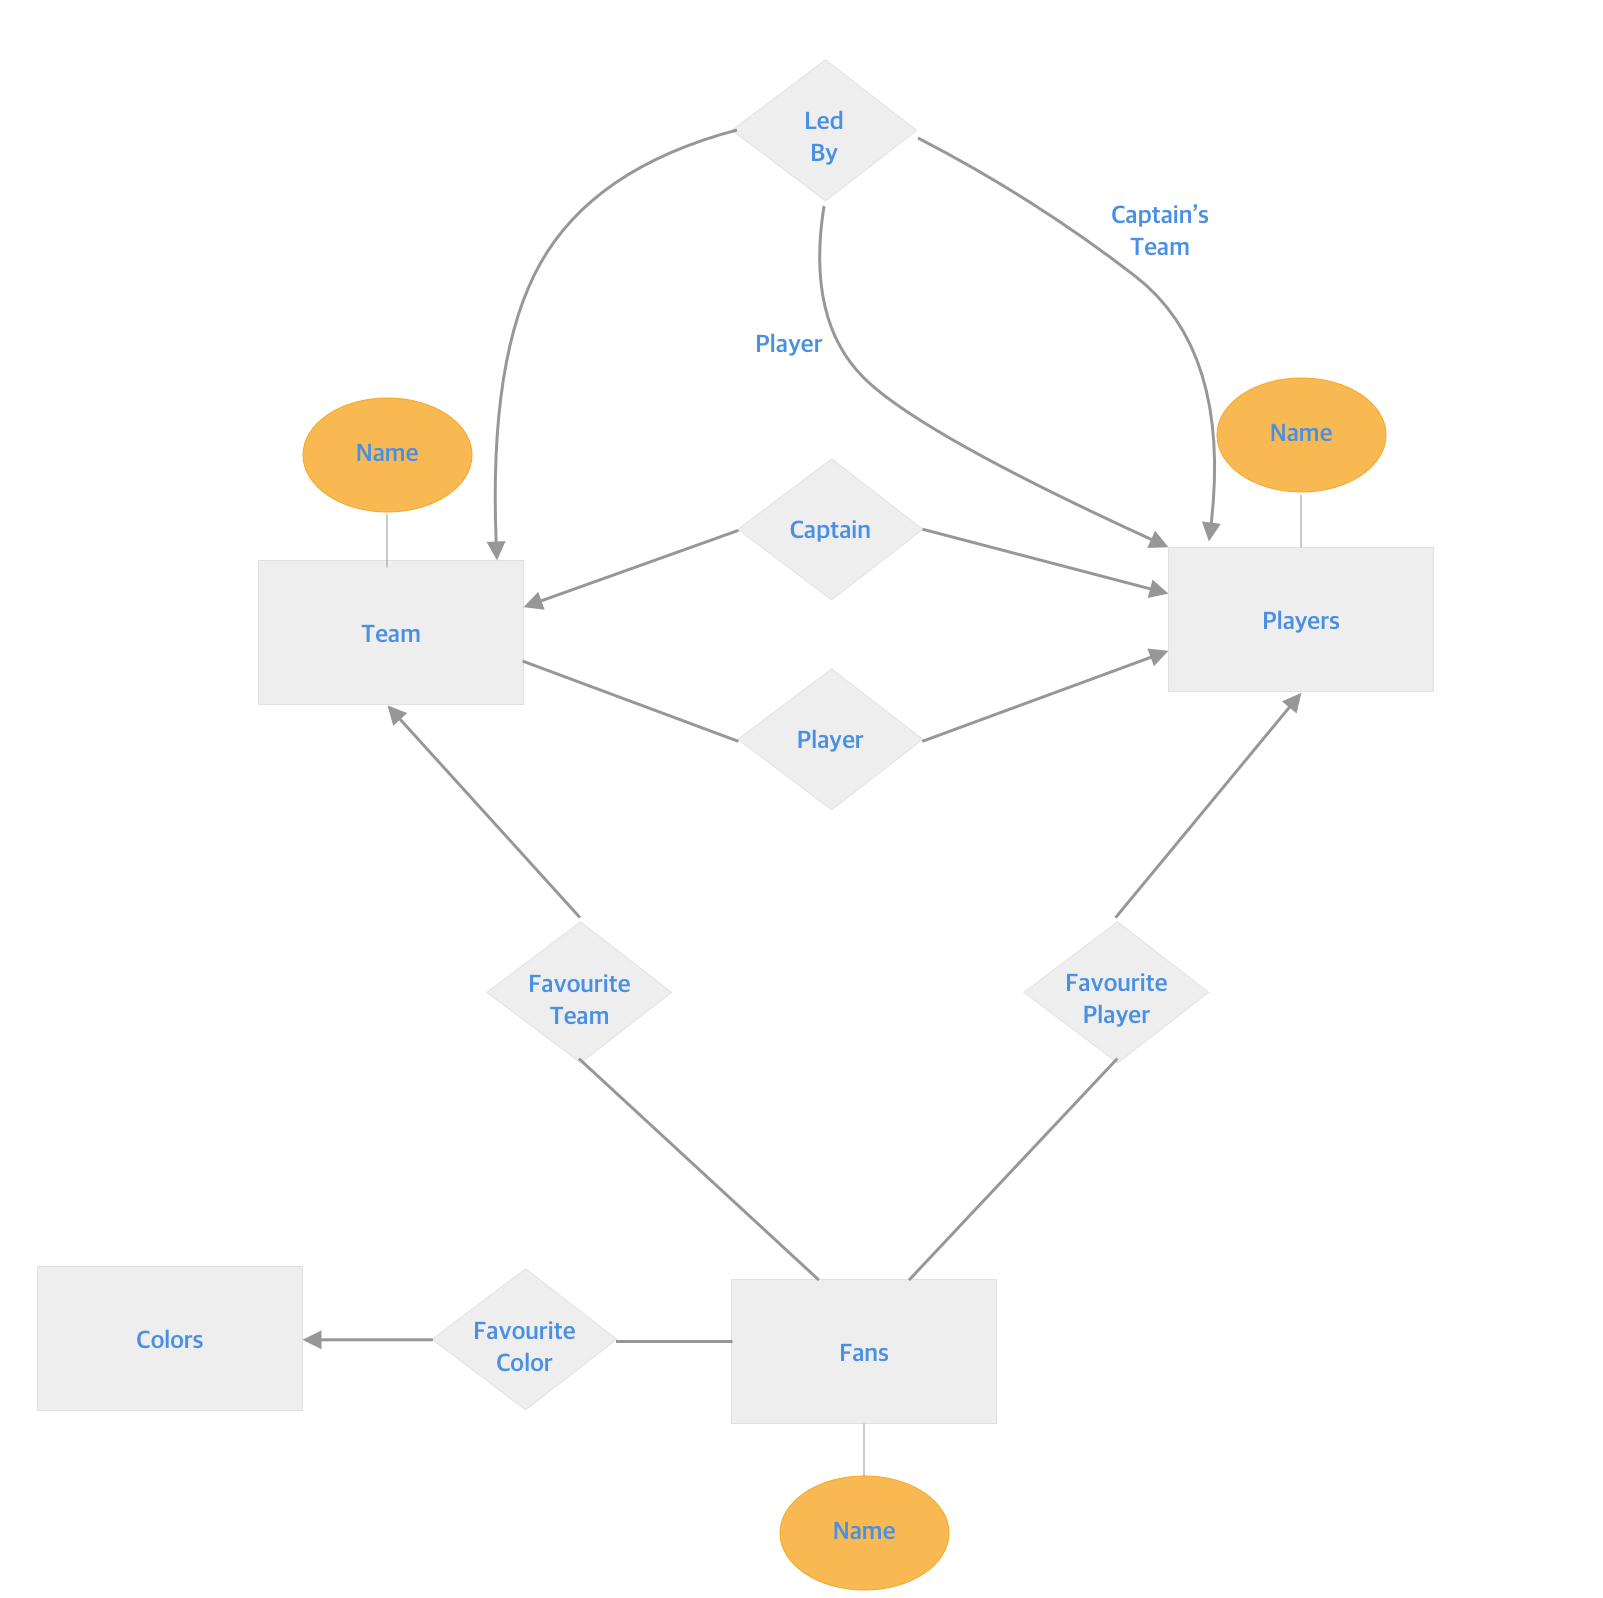
\includegraphics[width=\linewidth]{images/worksheet_14_solution_25.png}
        \end{center}

        \item

        \begin{center}
        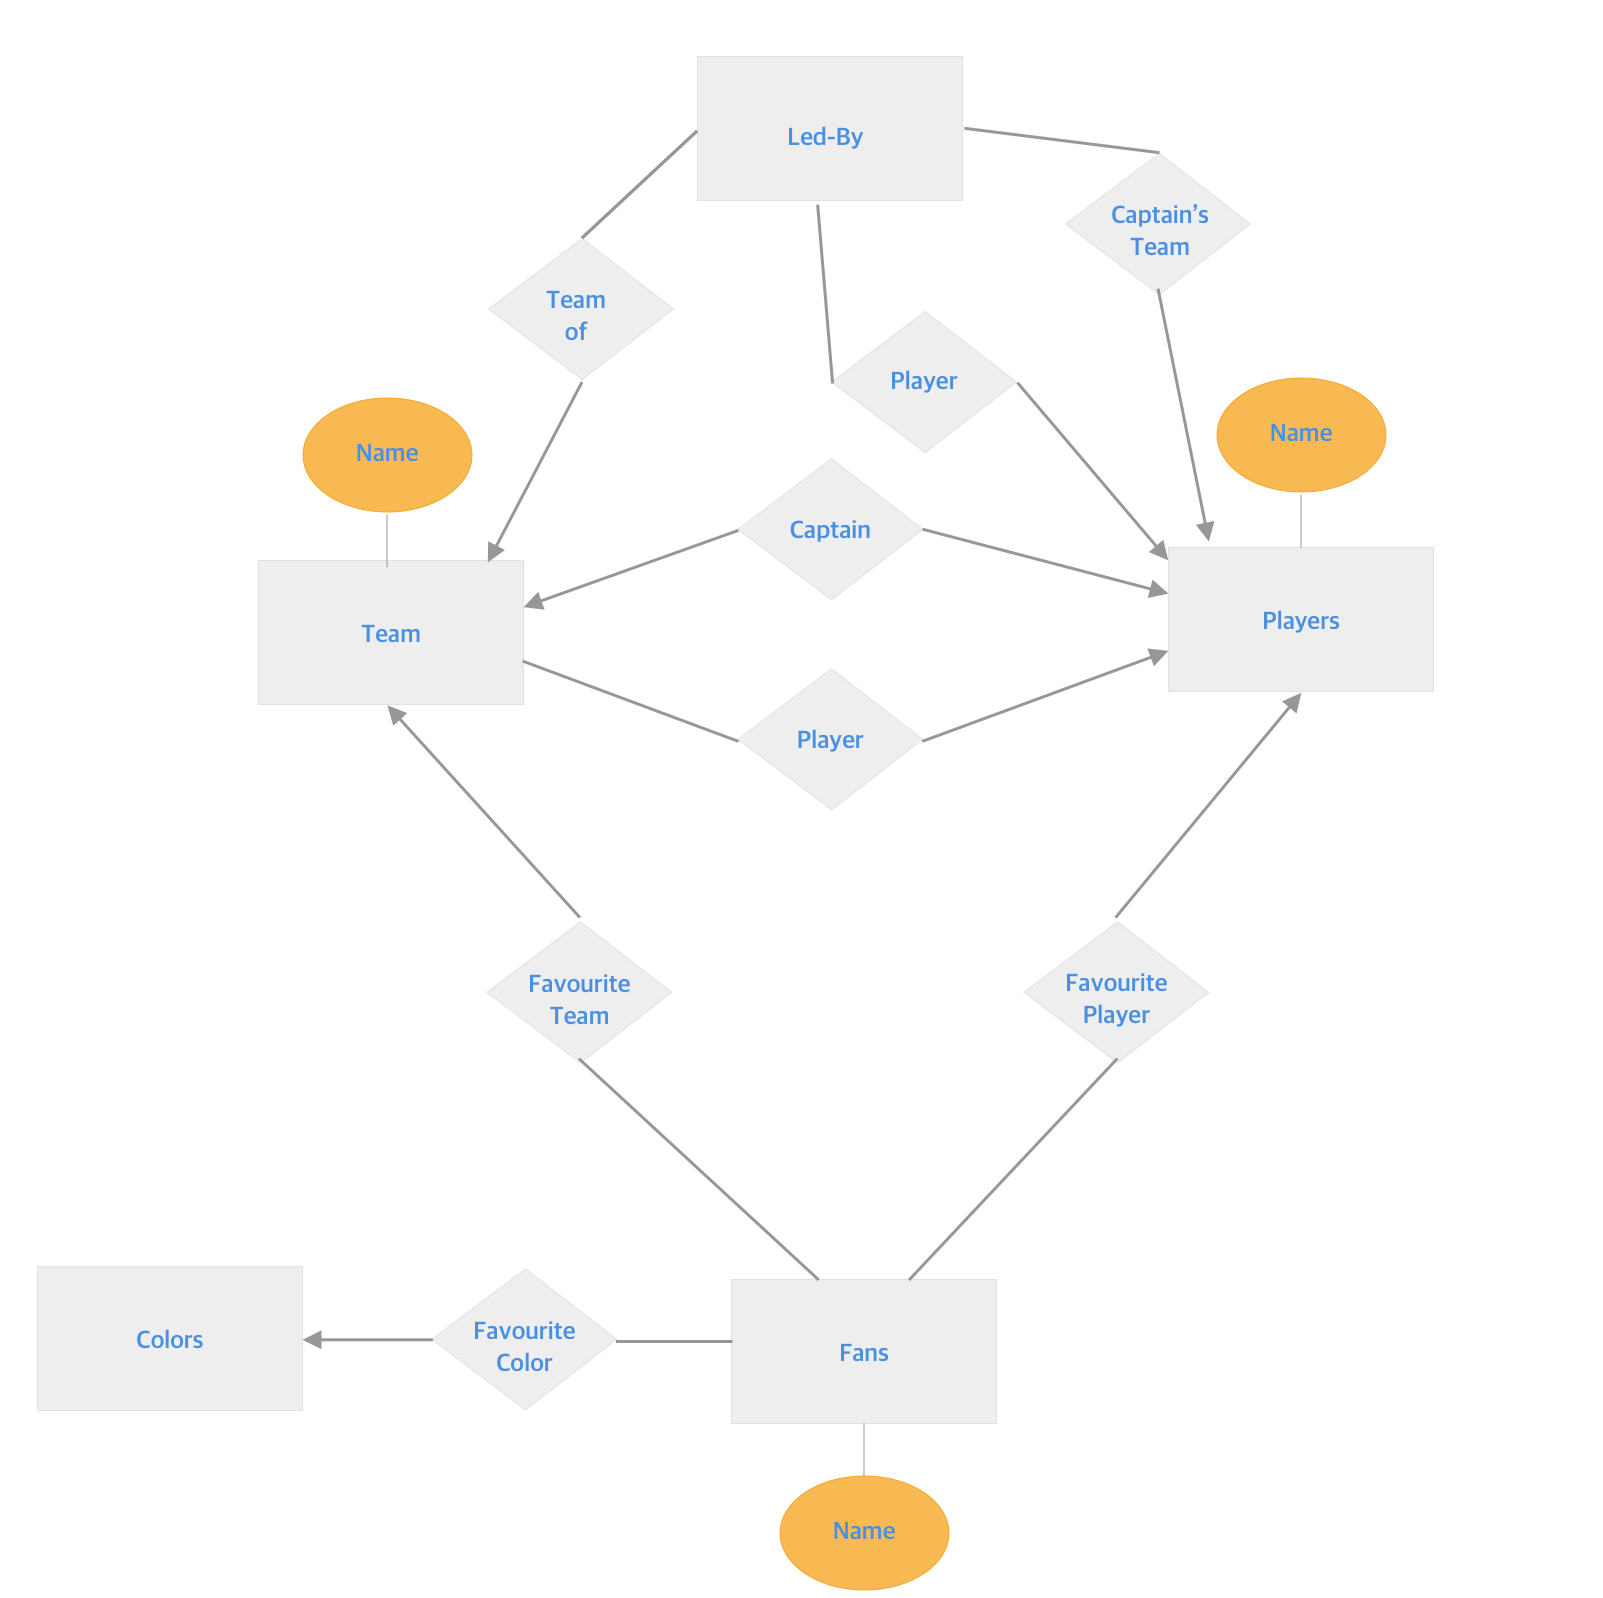
\includegraphics[width=\linewidth]{images/worksheet_14_solution_26.png}
        \end{center}

        \item

        They are the same. (I need more work on providing reason).


        \bigskip

        \underline{\textbf{Notes:}}

        \bigskip

        \begin{itemize}
            \item I should ask professor about this :'(
        \end{itemize}


    \end{enumerate}

    \item

    \begin{center}
    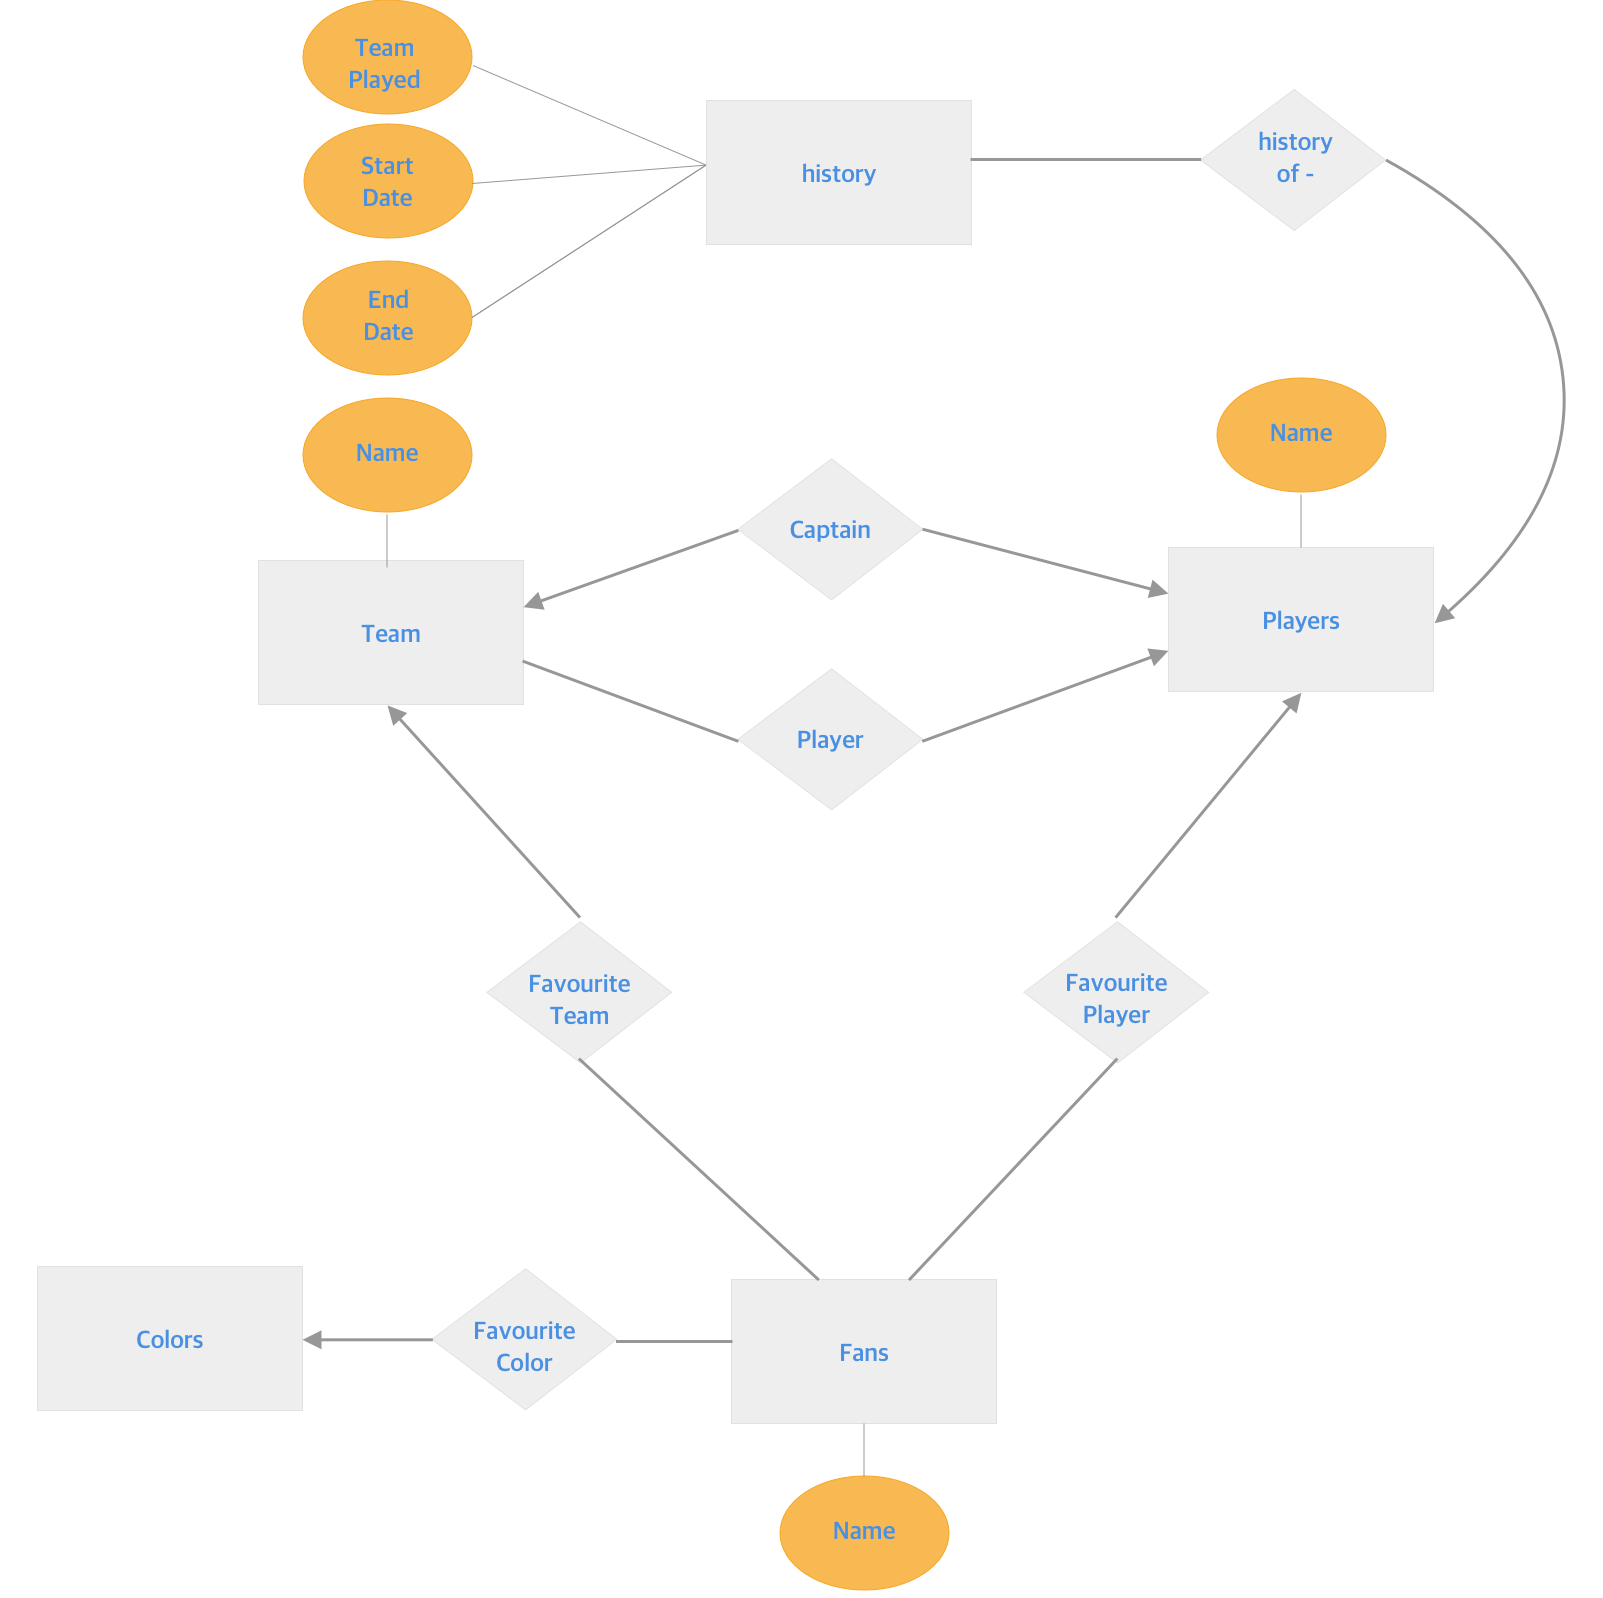
\includegraphics[width=\linewidth]{images/worksheet_14_solution_27.png}
    \end{center}

    \item

    \begin{center}
    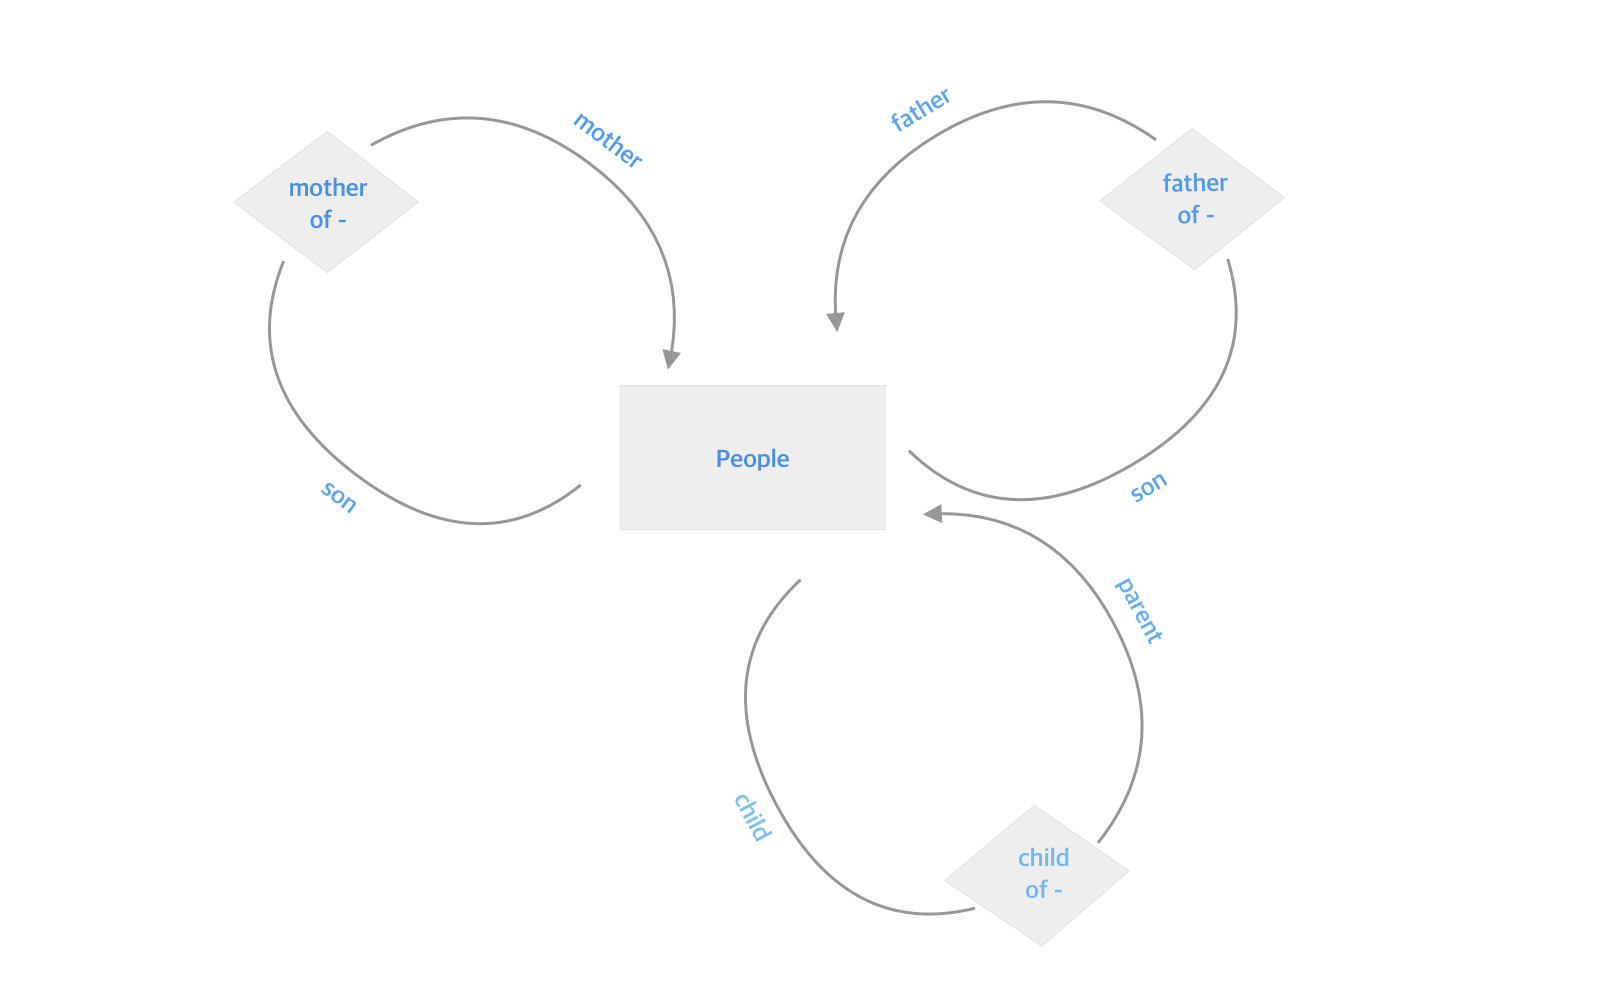
\includegraphics[width=\linewidth]{images/worksheet_14_solution_28.png}
    \end{center}


    \bigskip

    \begin{mdframed}
        \underline{\textbf{Correct Solution:}}

        \bigskip

        \begin{center}
        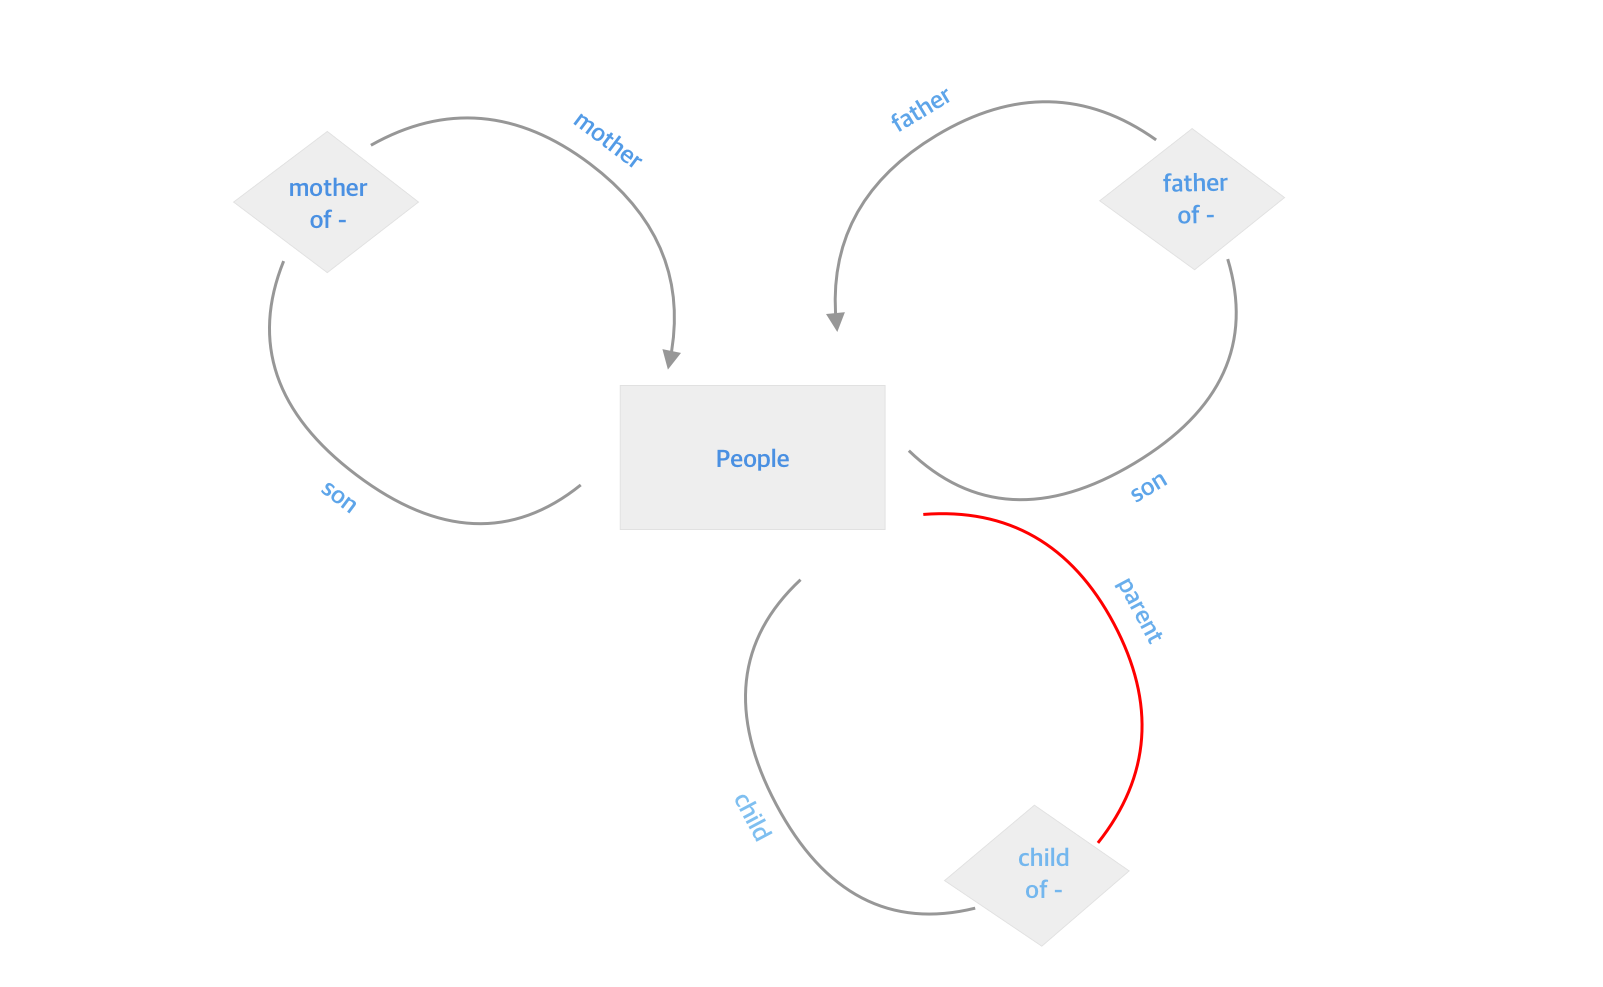
\includegraphics[width=\linewidth]{images/worksheet_14_solution_29.png}
        \end{center}
    \end{mdframed}

    \item

    \begin{center}
    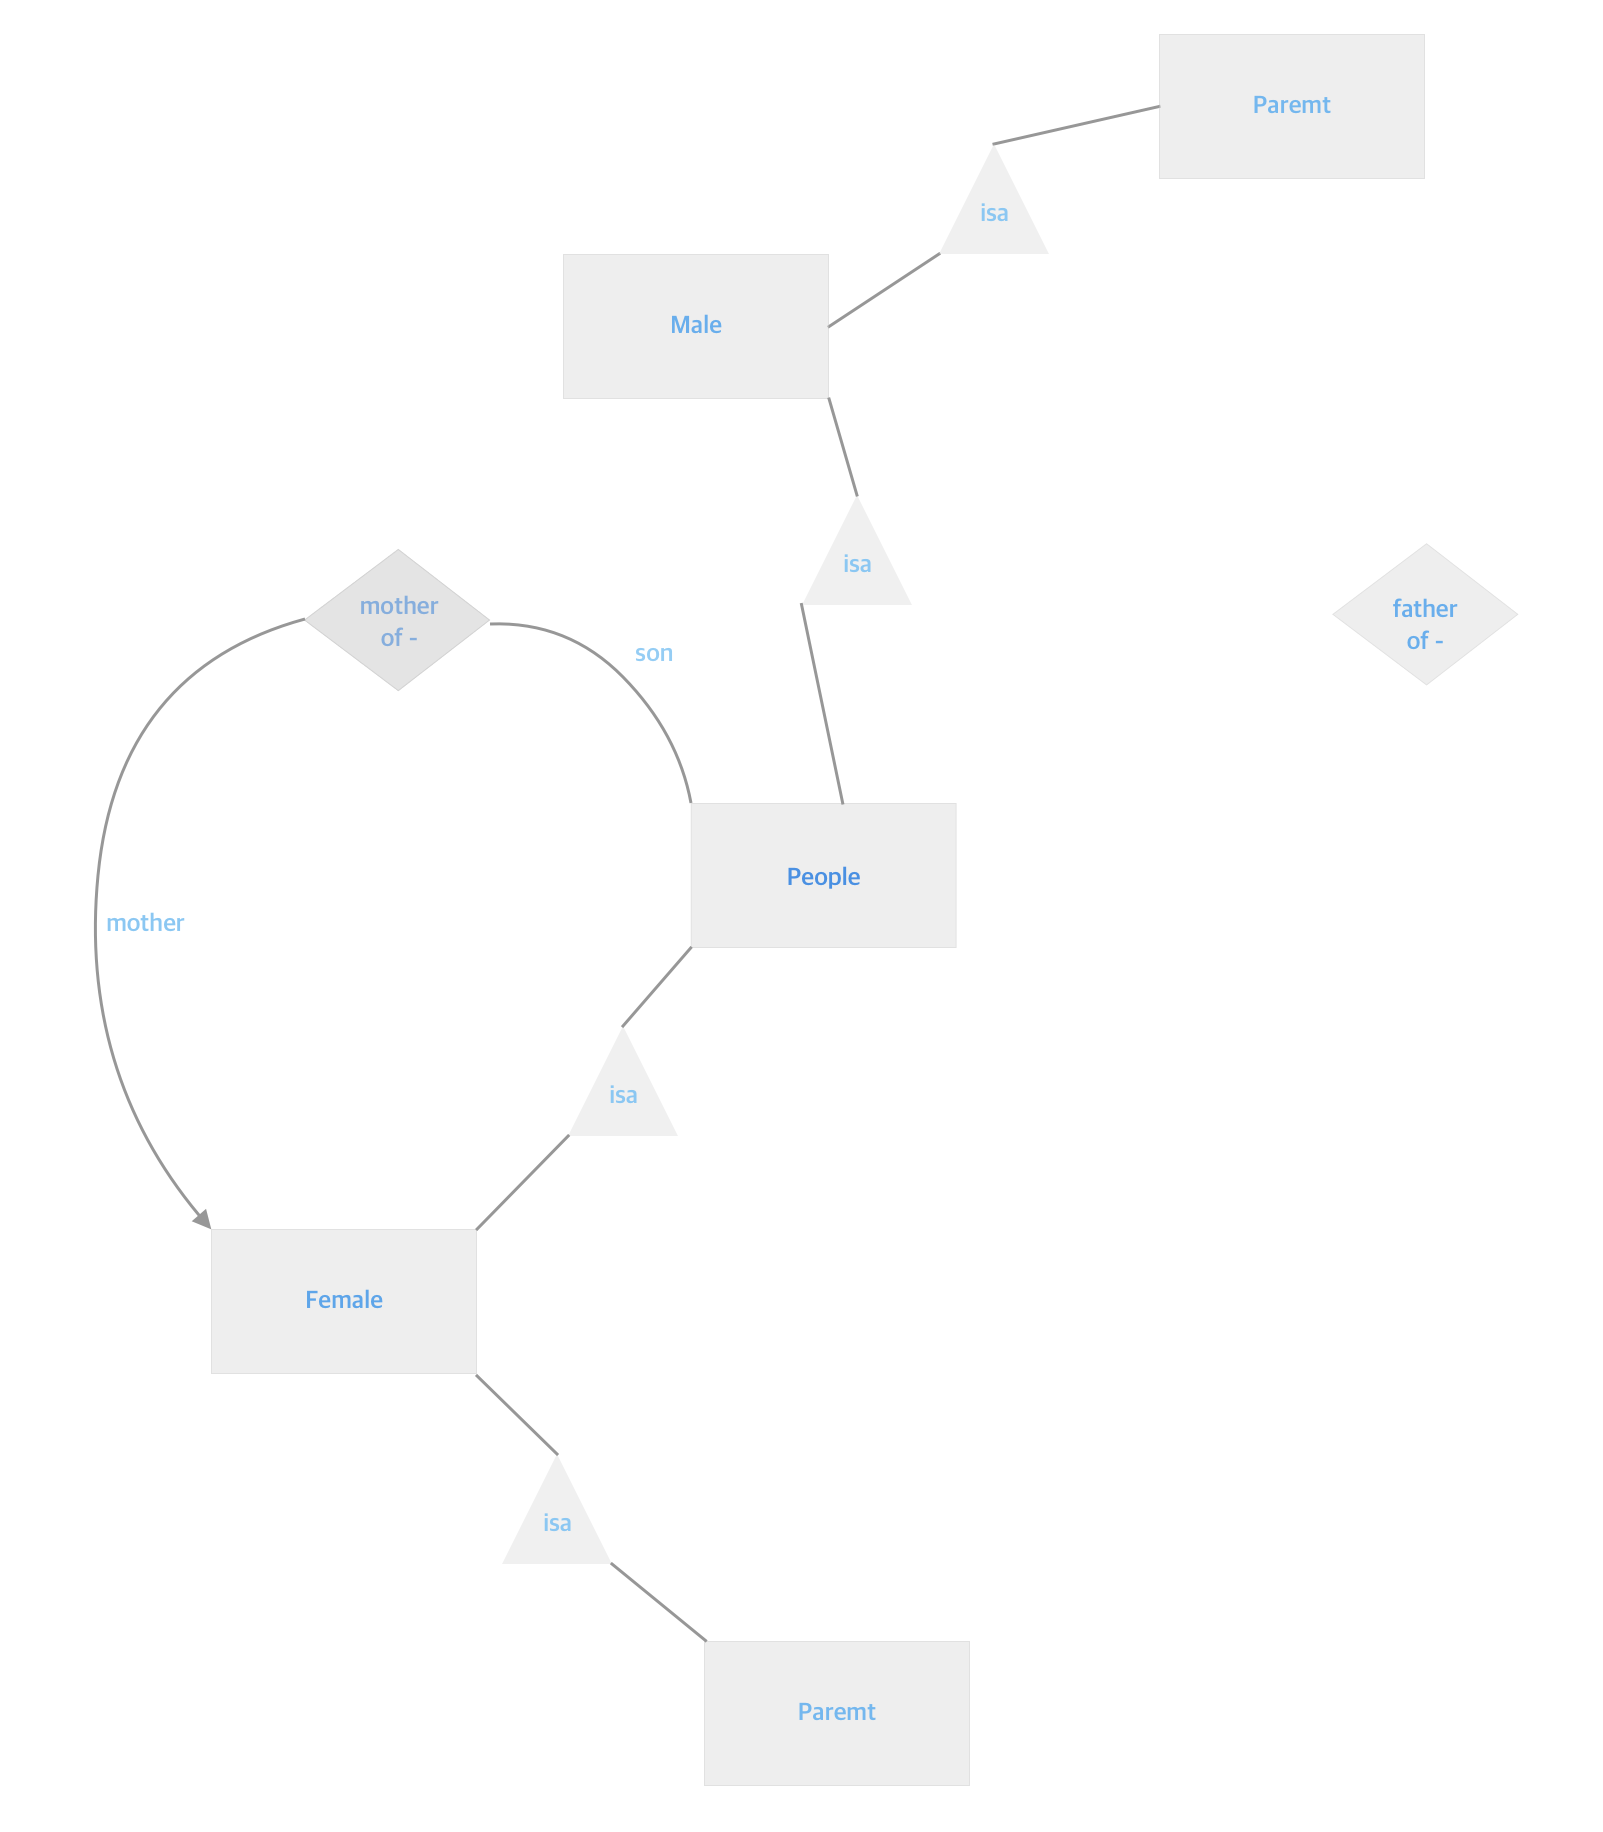
\includegraphics[width=\linewidth]{images/worksheet_14_solution_30.png}
    \end{center}

    \bigskip

    \underline{\textbf{Notes:}}

    \bigskip

    \begin{itemize}
        \item I feel the need to clarify with professor if two parent subclasses can
        exist
        \item I feel the need to ask professor whether this design is valid
    \end{itemize}

    \item

    \begin{enumerate}[a)]
        \item

        \begin{center}
        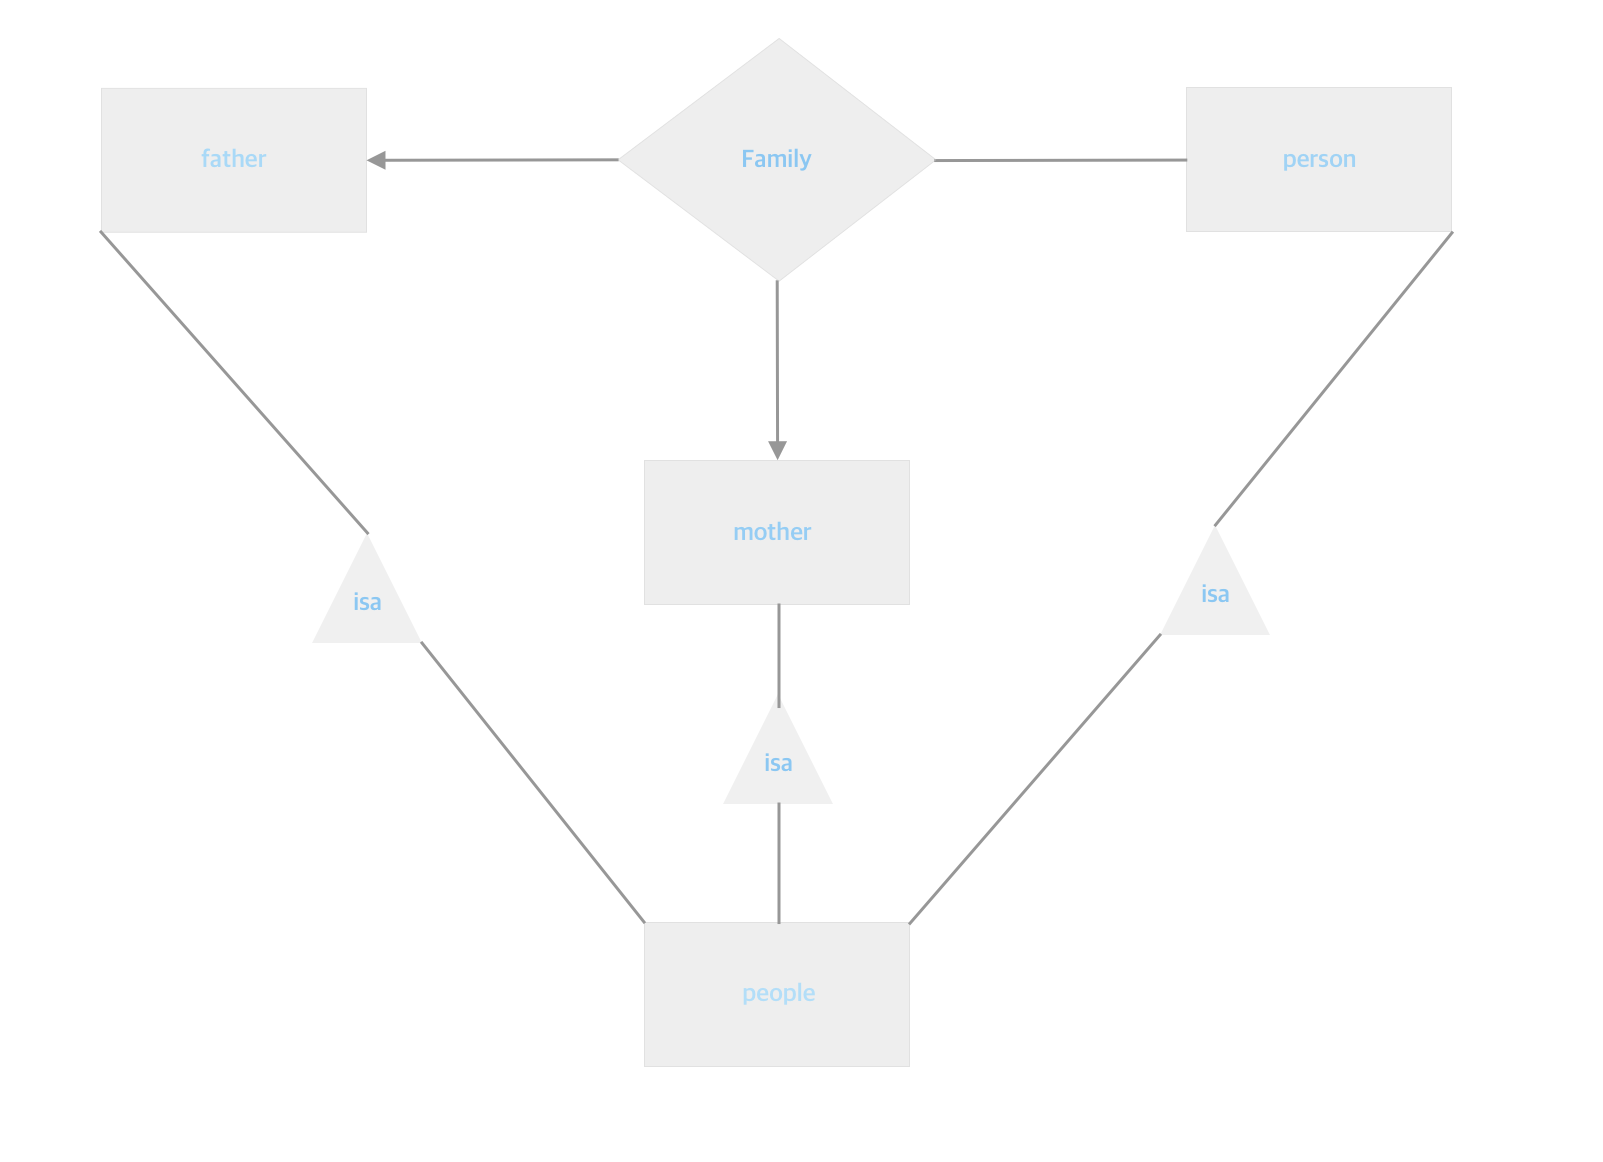
\includegraphics[width=\linewidth]{images/worksheet_14_solution_31.png}
        \end{center}

        \item

        \begin{center}
        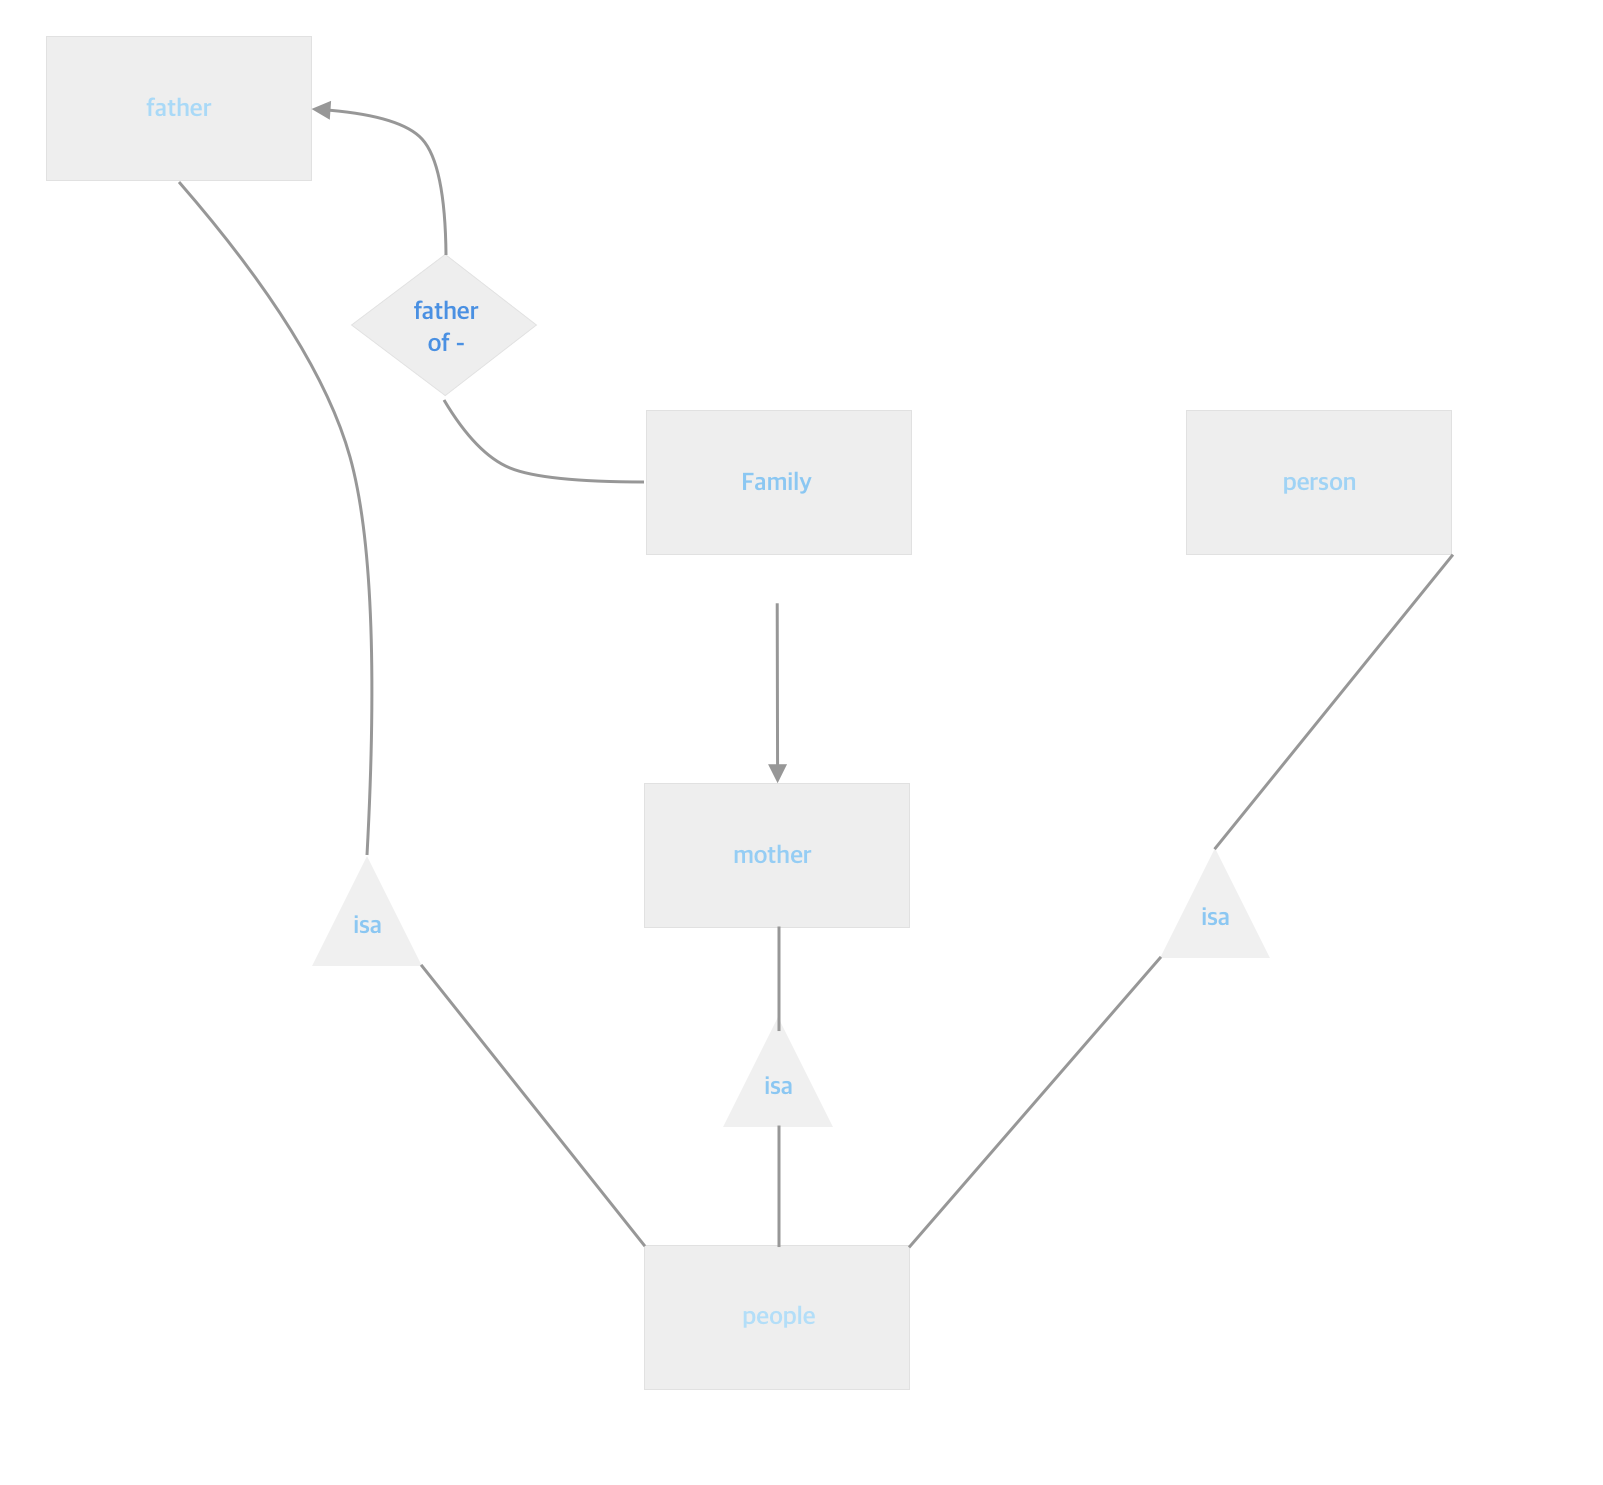
\includegraphics[width=\linewidth]{images/worksheet_14_solution_32.png}
        \end{center}

        \bigskip

        \underline{\textbf{Notes:}}

        \bigskip

        \begin{itemize}
            \item  I need to clarify with professor on one-to-many relationship.

            \bigskip

            Is it correct that the `one` side of `one-to-many' relationship represent
            foreign key in terms of SQL?

            \bigskip

            But how about the many side? What does it mean it to be many? so for example,
            ('Josh', 'Neville the father', 'Mary the mother'), ('Jay', 'Neville the father', 'Mary the mother'),
            is this one to many relationship?

            \bigskip

            In tabular terms / example what does one-to-many relationship represent
            in this context?
        \end{itemize}

    \end{enumerate}

    \item

    \begin{center}
    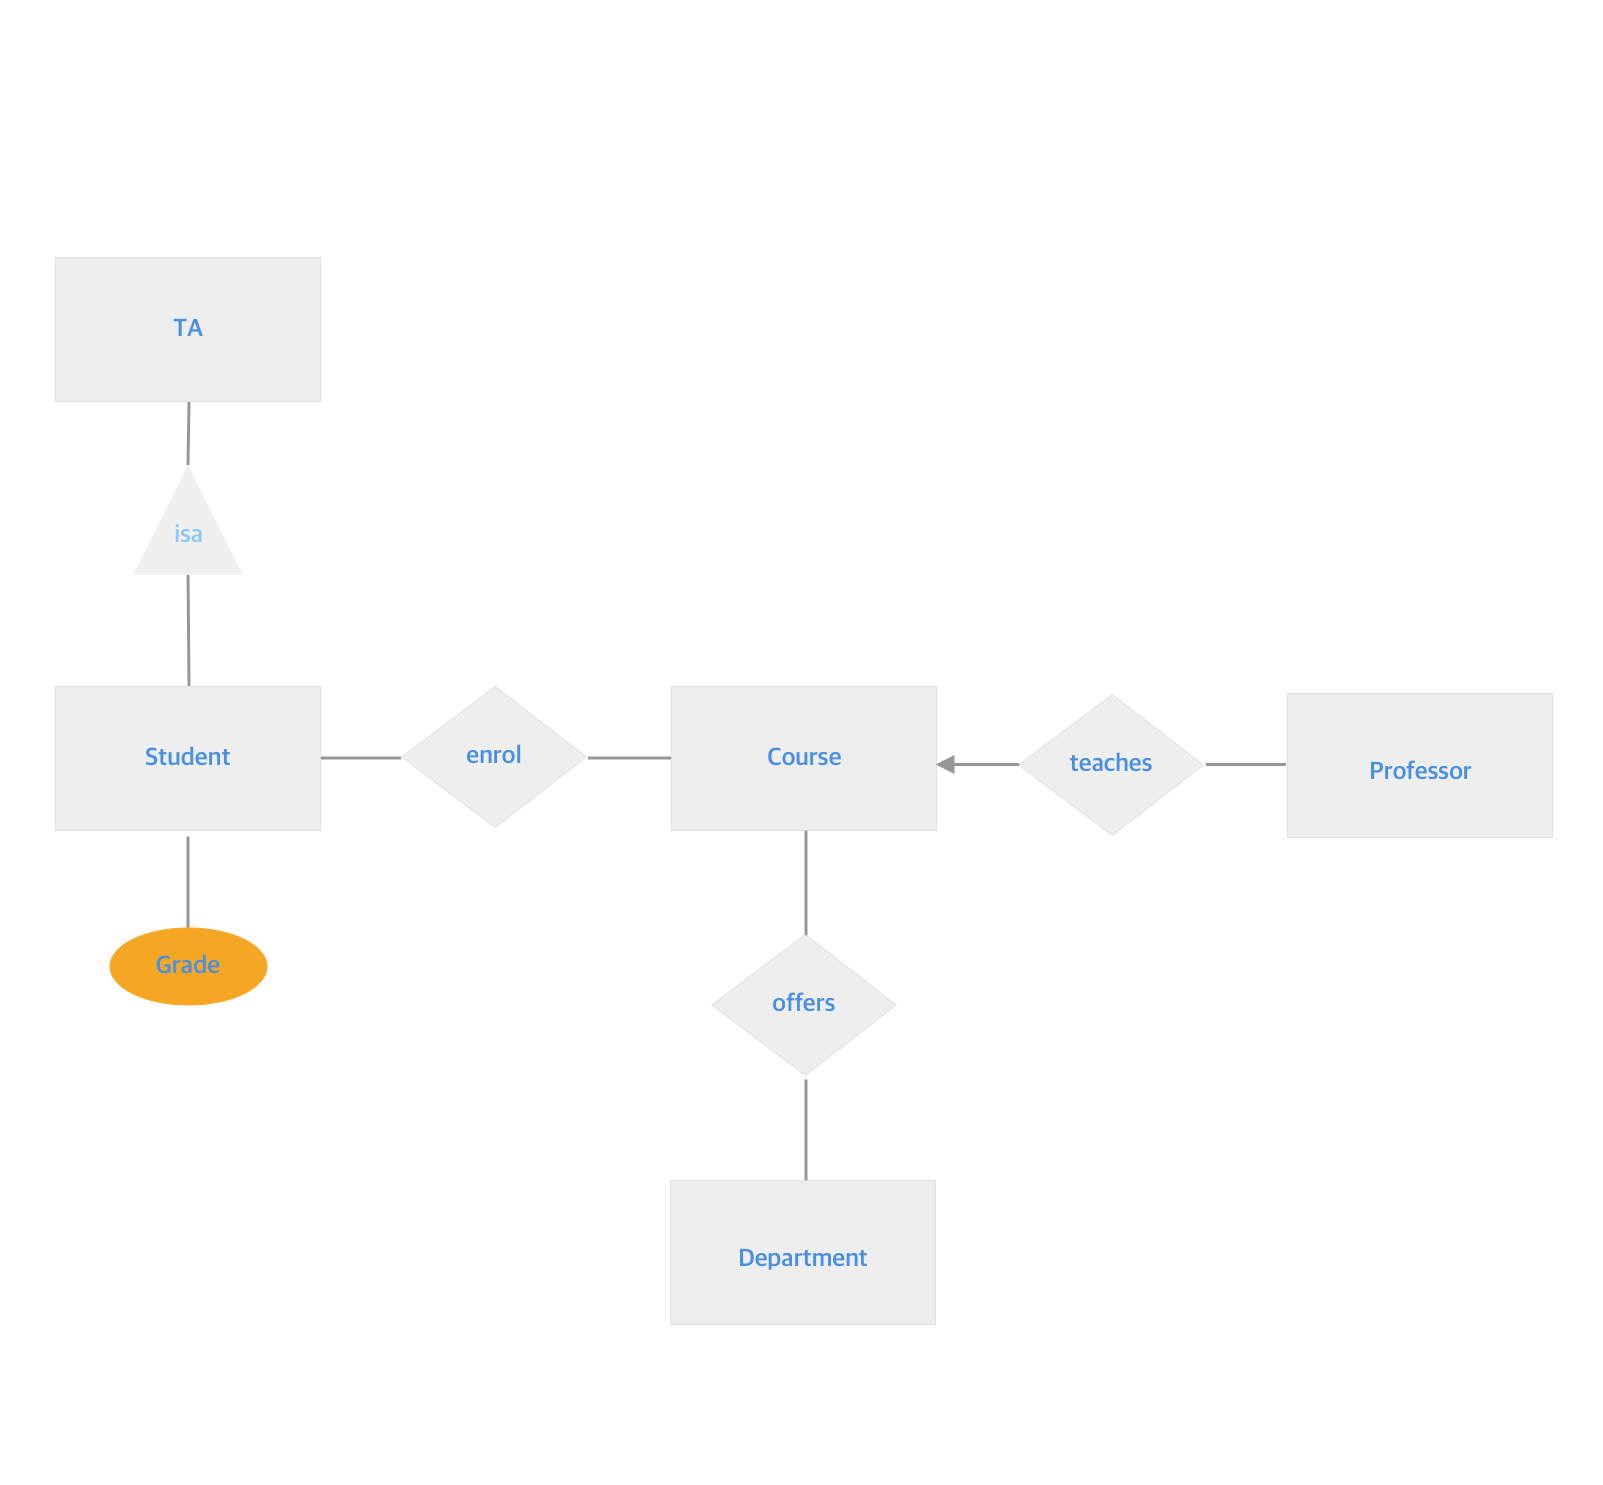
\includegraphics[width=\linewidth]{images/worksheet_14_solution_33.png}
    \end{center}

    \item

    \begin{center}
    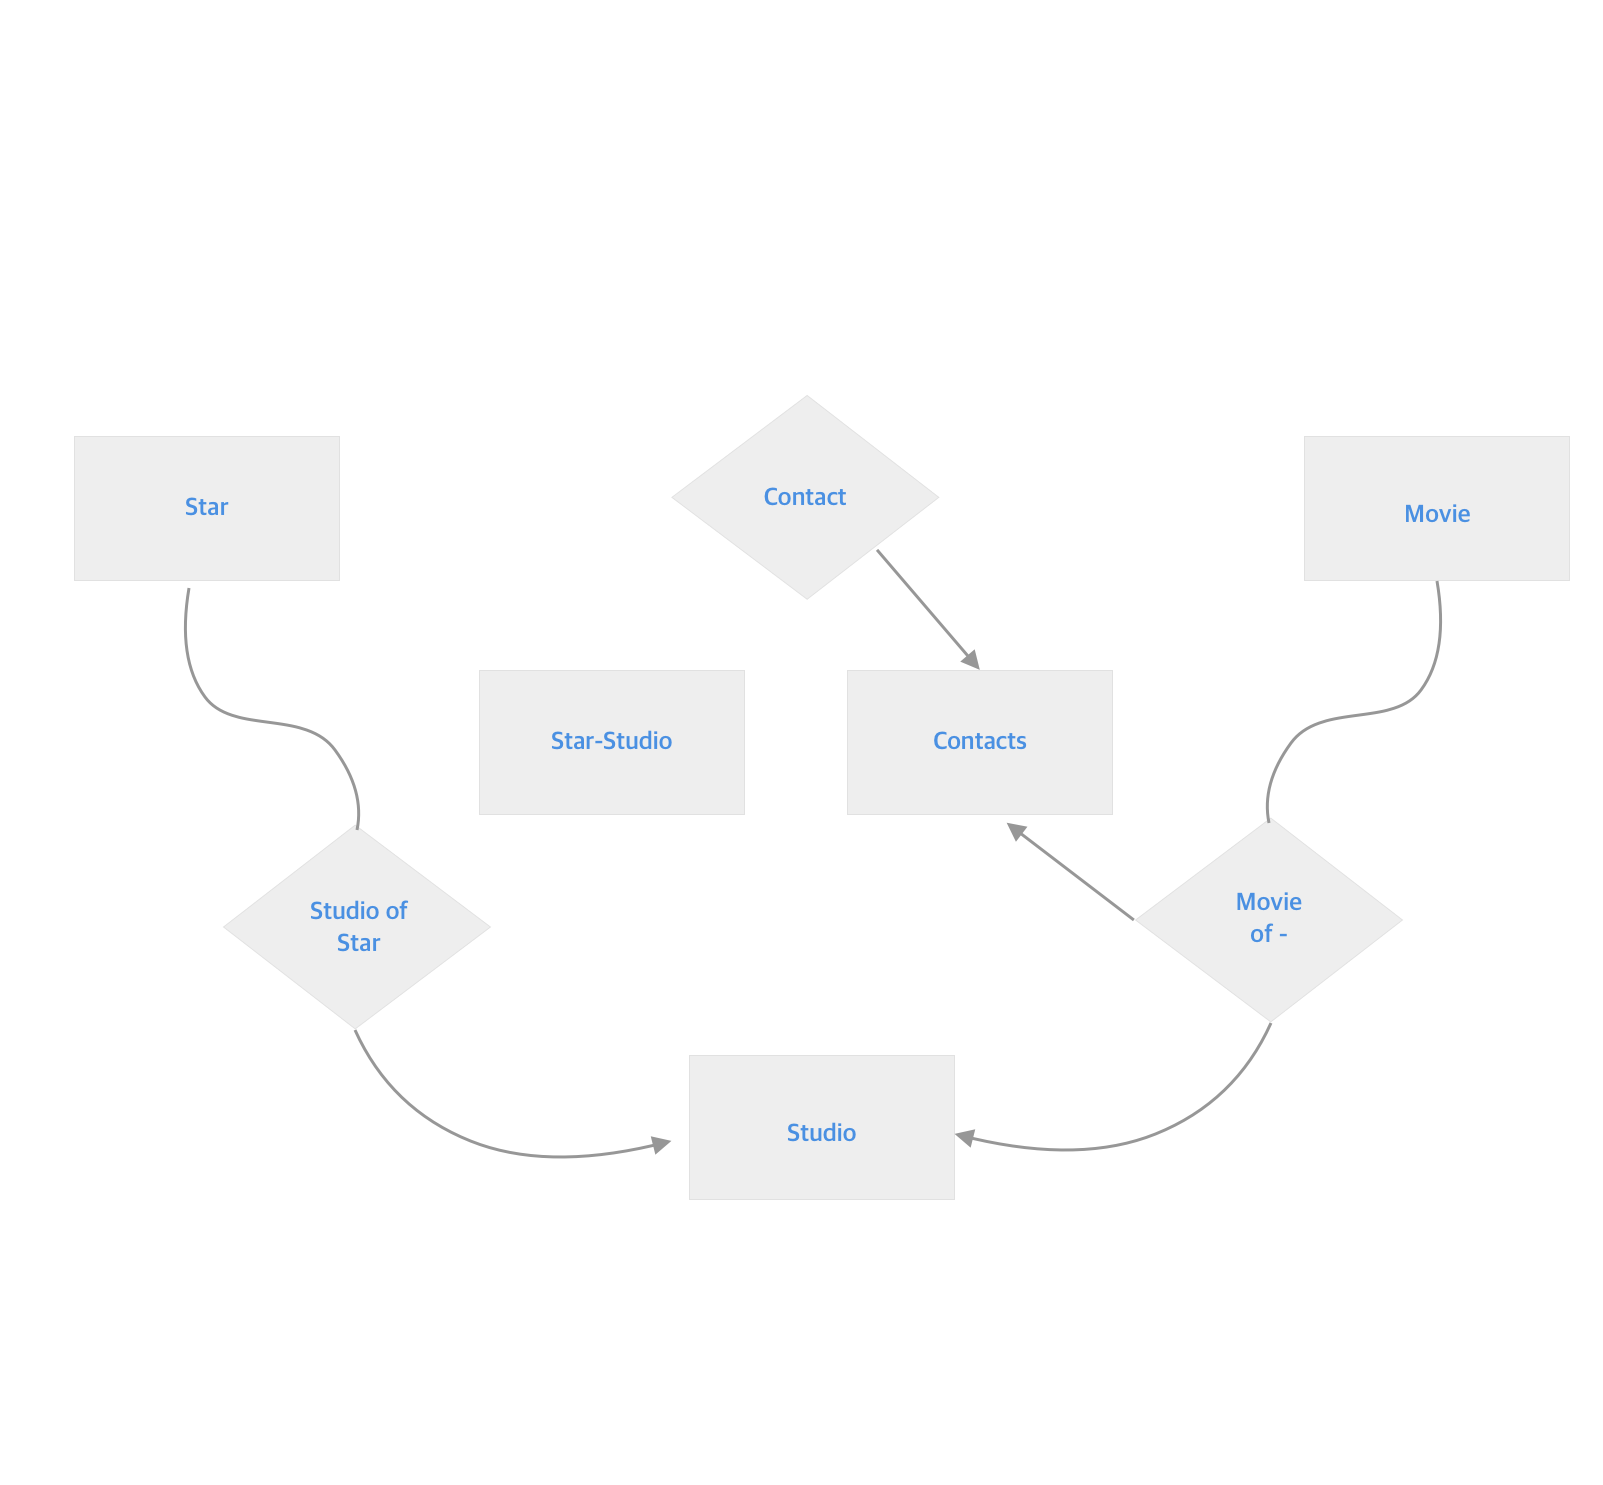
\includegraphics[width=\linewidth]{images/worksheet_14_solution_34.png}
    \end{center}

    \bigskip

    \begin{mdframed}
        \underline{\textbf{Correct Solution:}}

        \bigskip

        \begin{center}
        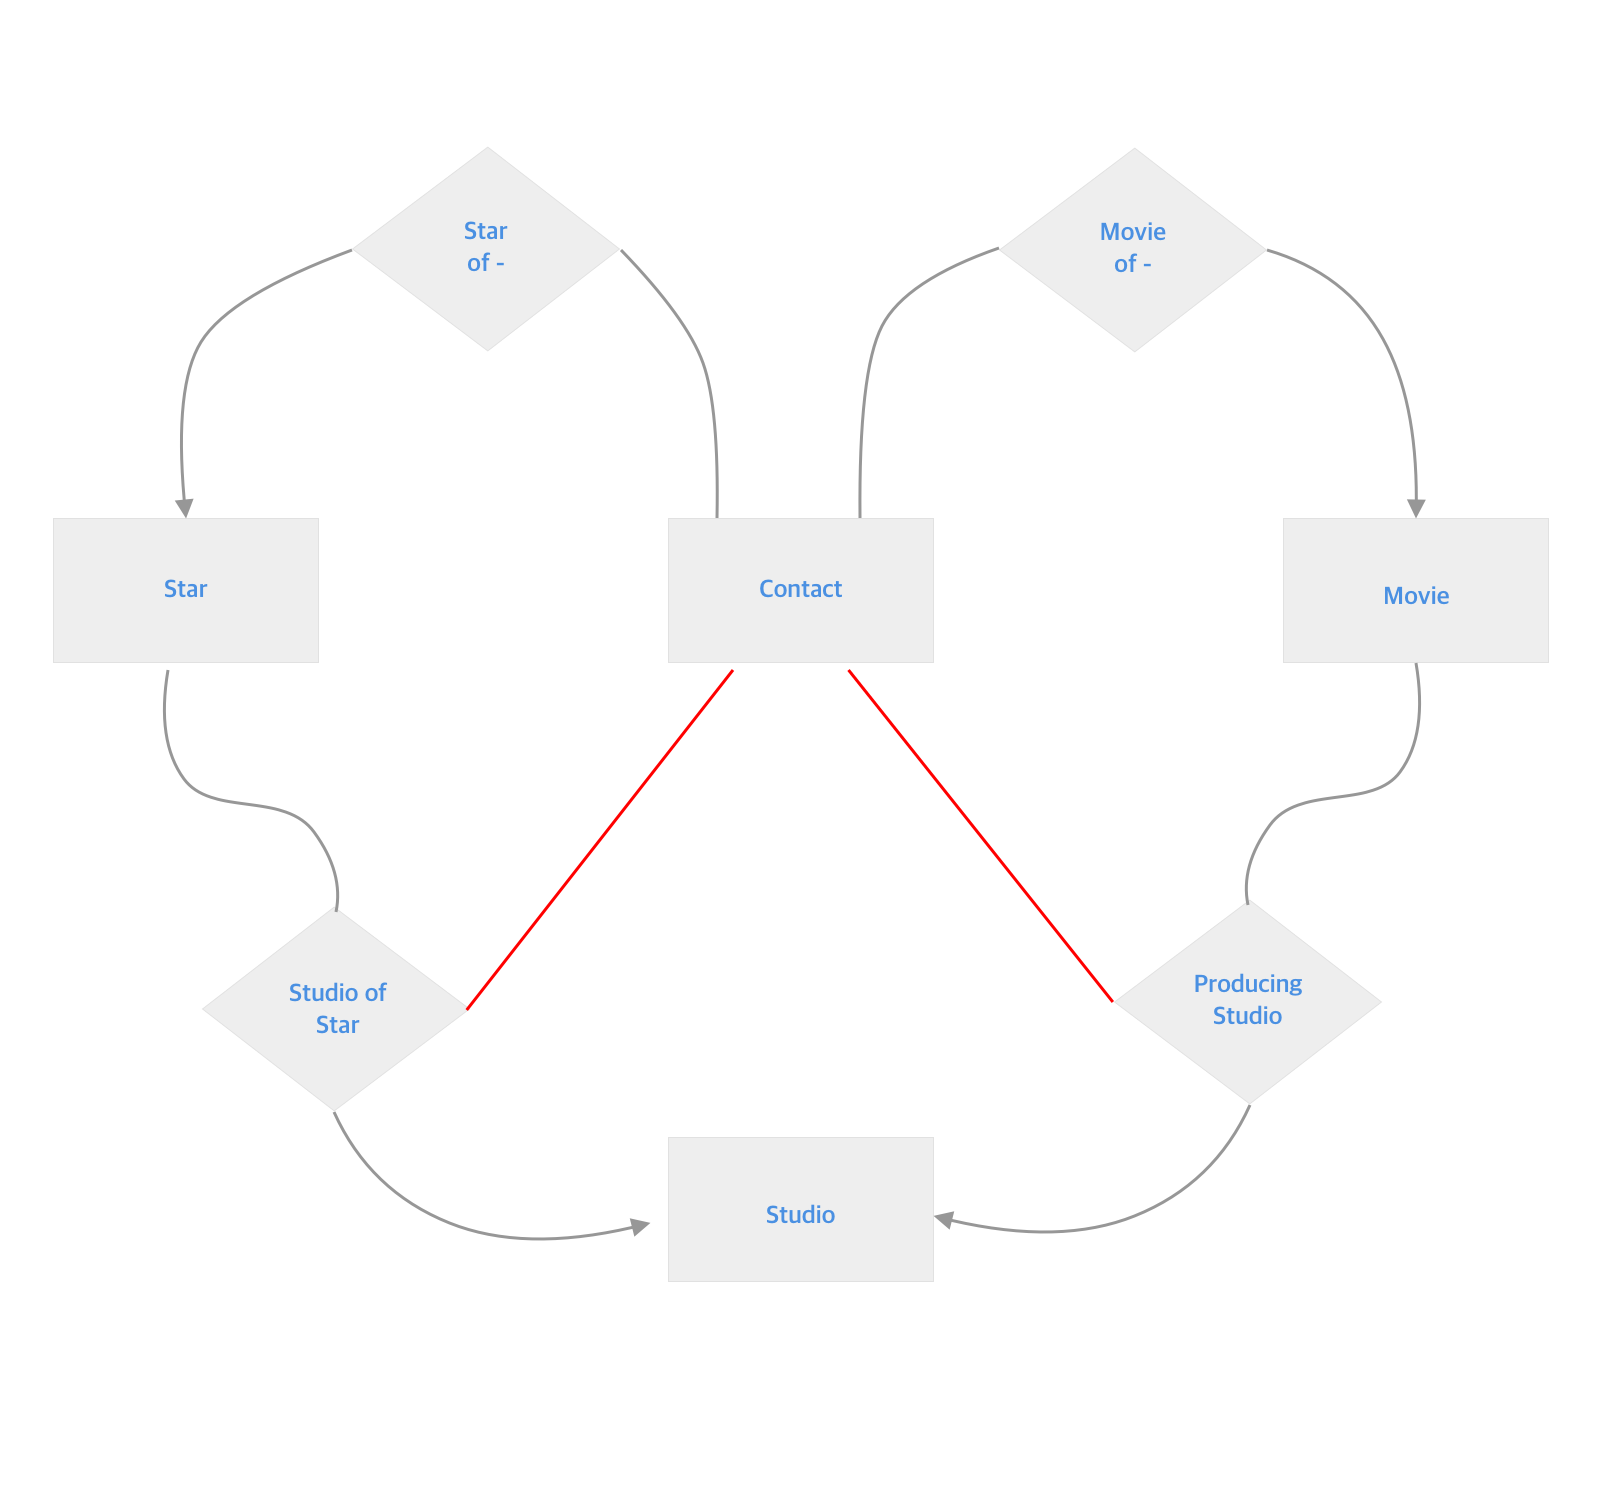
\includegraphics[width=\linewidth]{images/worksheet_14_solution_35.png}
        \end{center}

    \end{mdframed}

    \item

    \bigskip

    Simplicity count is violated. There is more than necessary number of entitiy sets
    and attributs for address and accounts.

    \bigskip

    \begin{center}
    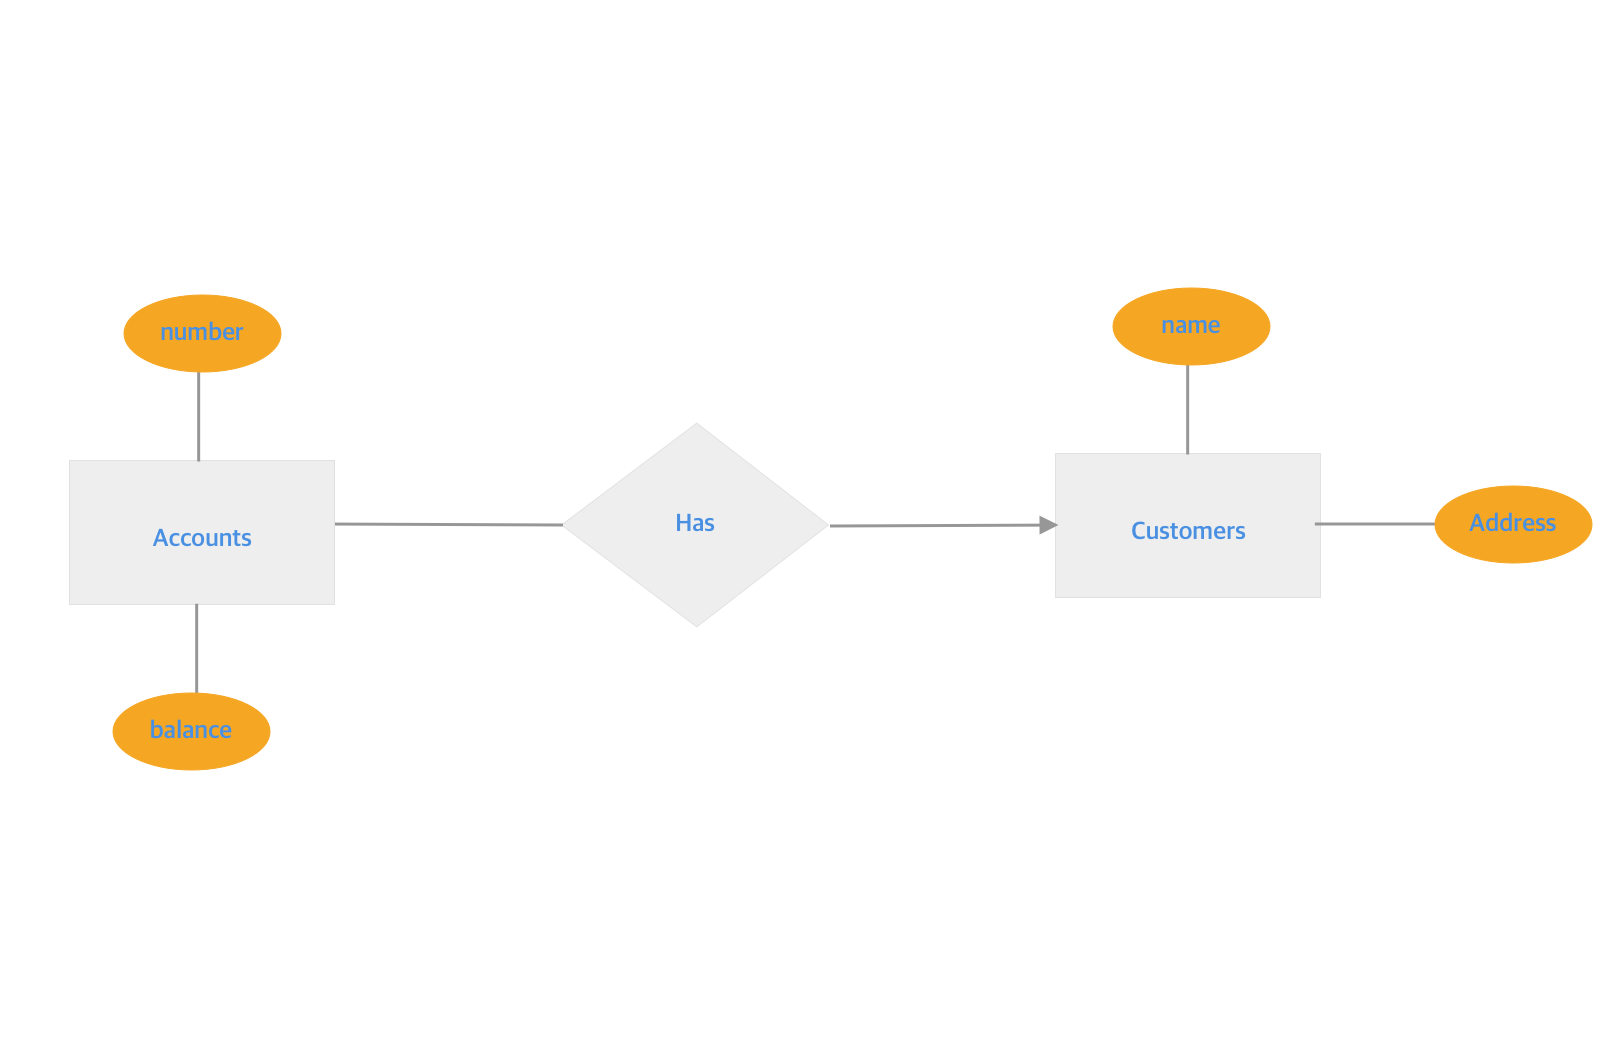
\includegraphics[width=\linewidth]{images/worksheet_14_solution_38.png}
    \end{center}


    \bigskip

    \underline{\textbf{Notes:}}

    \bigskip

    \begin{itemize}
        \item Design Principles

        \begin{enumerate}[1.]
            \item Faithfulness

            \begin{itemize}
                \item means design should make sense and meet its specification
                \item e.g. Adding attribute \textit{number-of-cylinders} to \textit{Stars} $\to$ NONO
            \end{itemize}

            \item Avoiding Redundancy

            \begin{itemize}
                \item \textit{Redundancy} means saying the same thing in
                two (or more) different ways
            \end{itemize}

            \bigskip

            \underline{\textbf{Example (The good example):}}

            \bigskip

            \begin{center}
            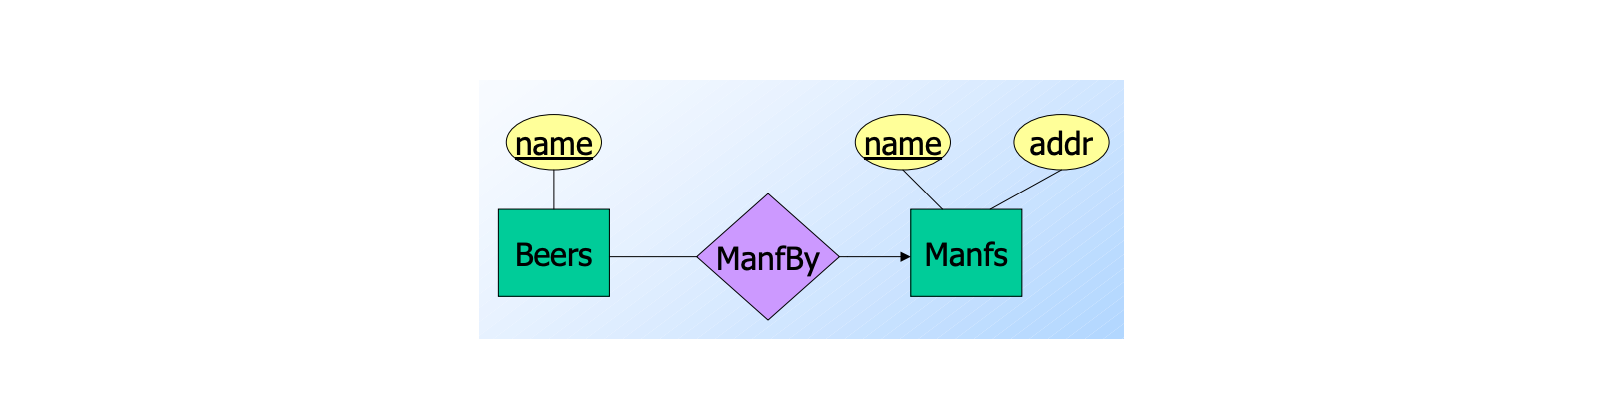
\includegraphics[width=\linewidth]{images/worksheet_14_solution_36.png}
            \end{center}

            \bigskip

            \underline{\textbf{Example (The bad example):}}

            \bigskip

            \begin{center}
            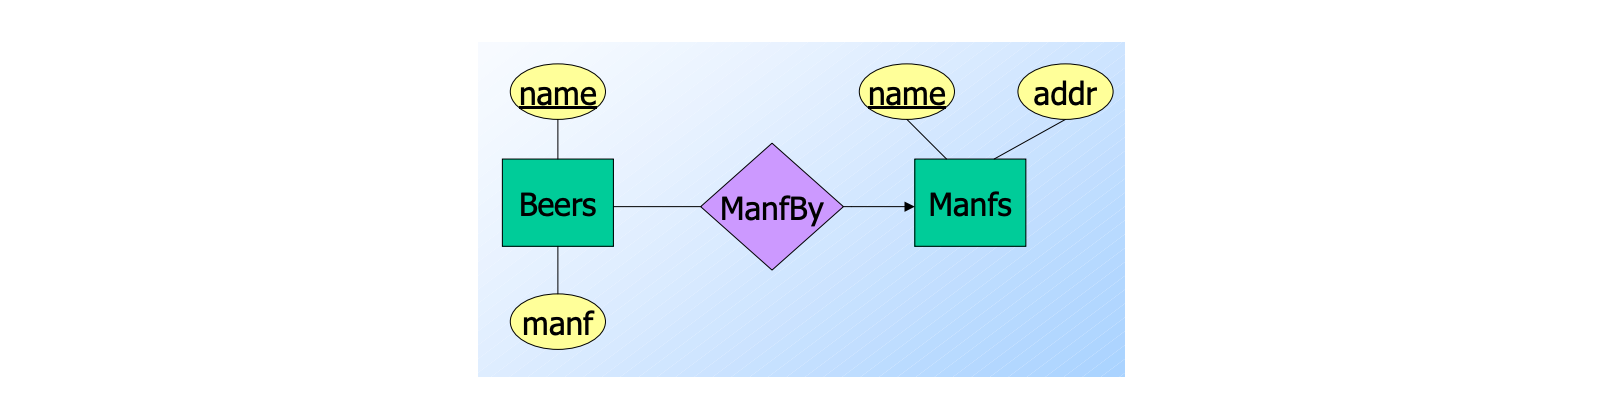
\includegraphics[width=\linewidth]{images/worksheet_14_solution_37.png}
            \end{center}

            \item Simplicty Counts

            \begin{itemize}
                \item Avoid adding more more elements than necessary
            \end{itemize}
            \item Choosing the Right Relationships

            \begin{itemize}
                \item Don't add relationships more than necessary
            \end{itemize}

            \item Picking the Right Kind of Element

            \begin{itemize}
                \item Many of the choices are between using attributes and using
                entity set / relationship combinations
            \end{itemize}
        \end{enumerate}
    \end{itemize}

    \item

    They should be combined when each studio has unique president

    \item

    \underline{\textbf{Solution:}}

    \bigskip

    \begin{center}
    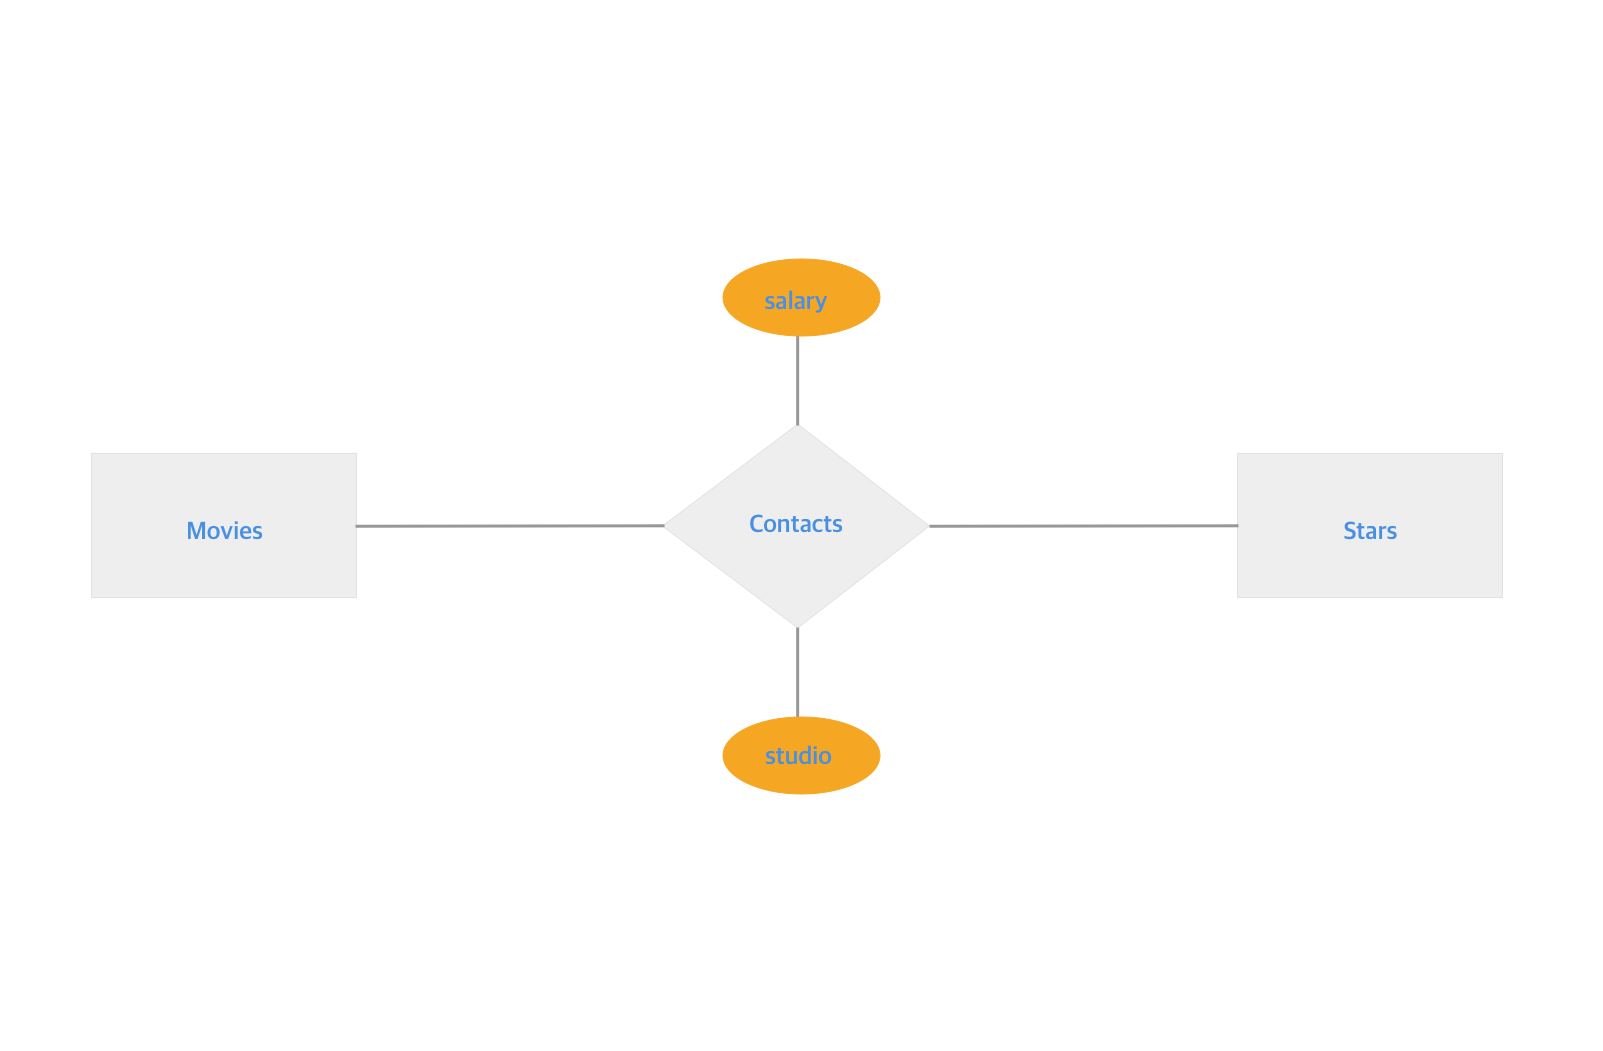
\includegraphics[width=\linewidth]{images/worksheet_14_solution_39.png}
    \end{center}

    \item

    \begin{enumerate}[a)]
        \item \underline{\textbf{Solution:}}

        \bigskip

        \begin{center}
        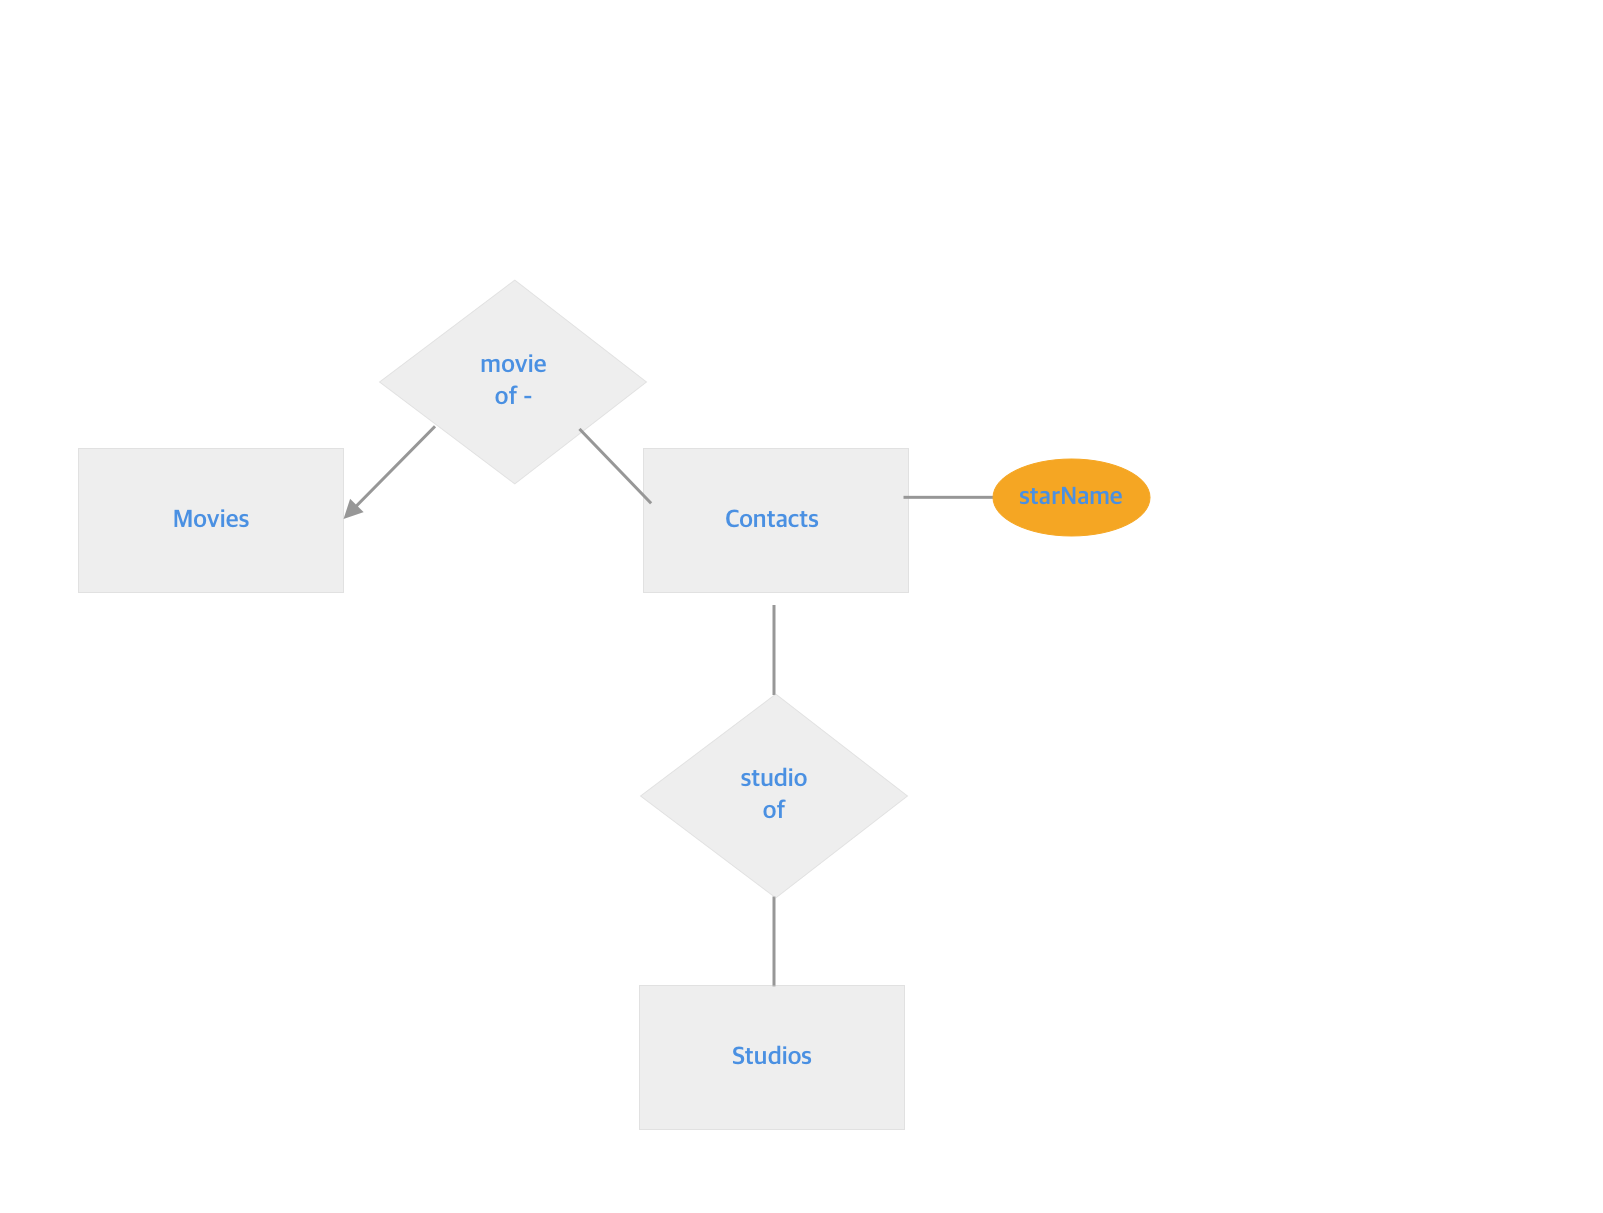
\includegraphics[width=\linewidth]{images/worksheet_14_solution_40.png}
        \end{center}

        \item \underline{\textbf{Solution:}}

        \bigskip

        \begin{center}
        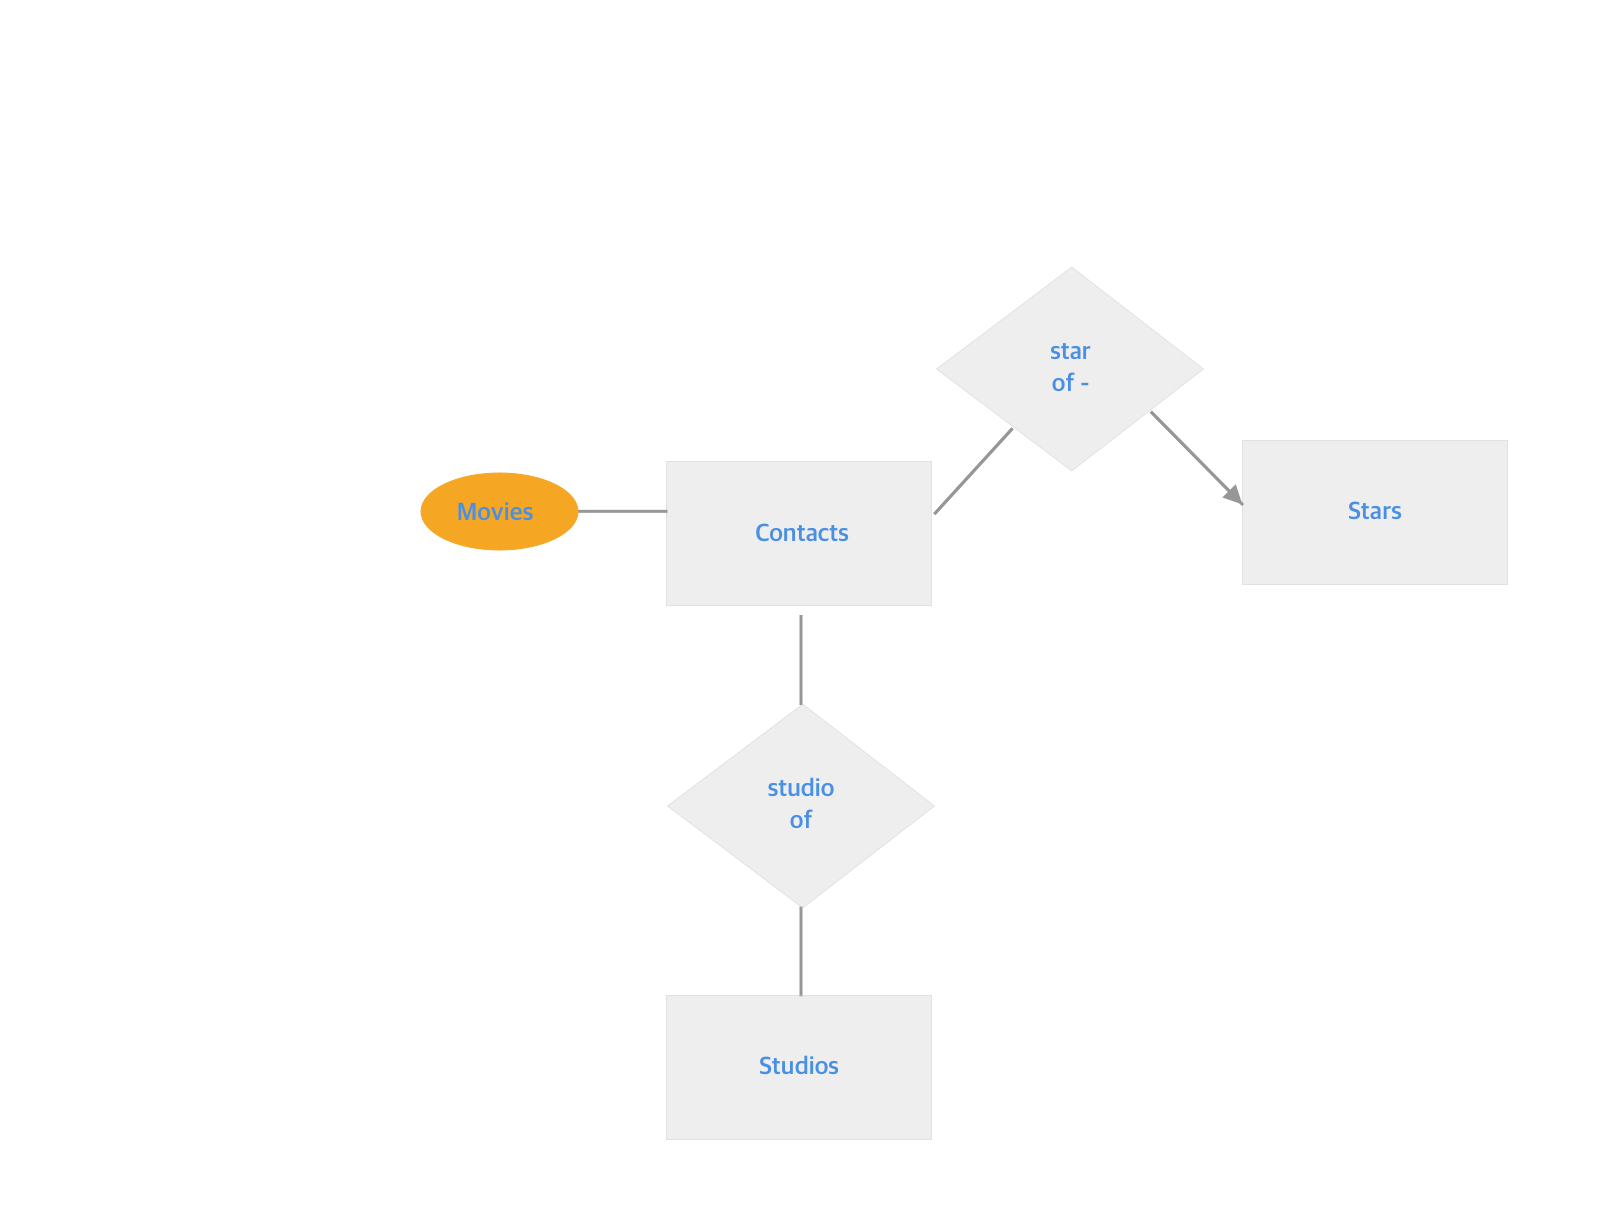
\includegraphics[width=\linewidth]{images/worksheet_14_solution_41.png}
        \end{center}

        \item \underline{\textbf{Solution:}}

        \bigskip

        \begin{center}
        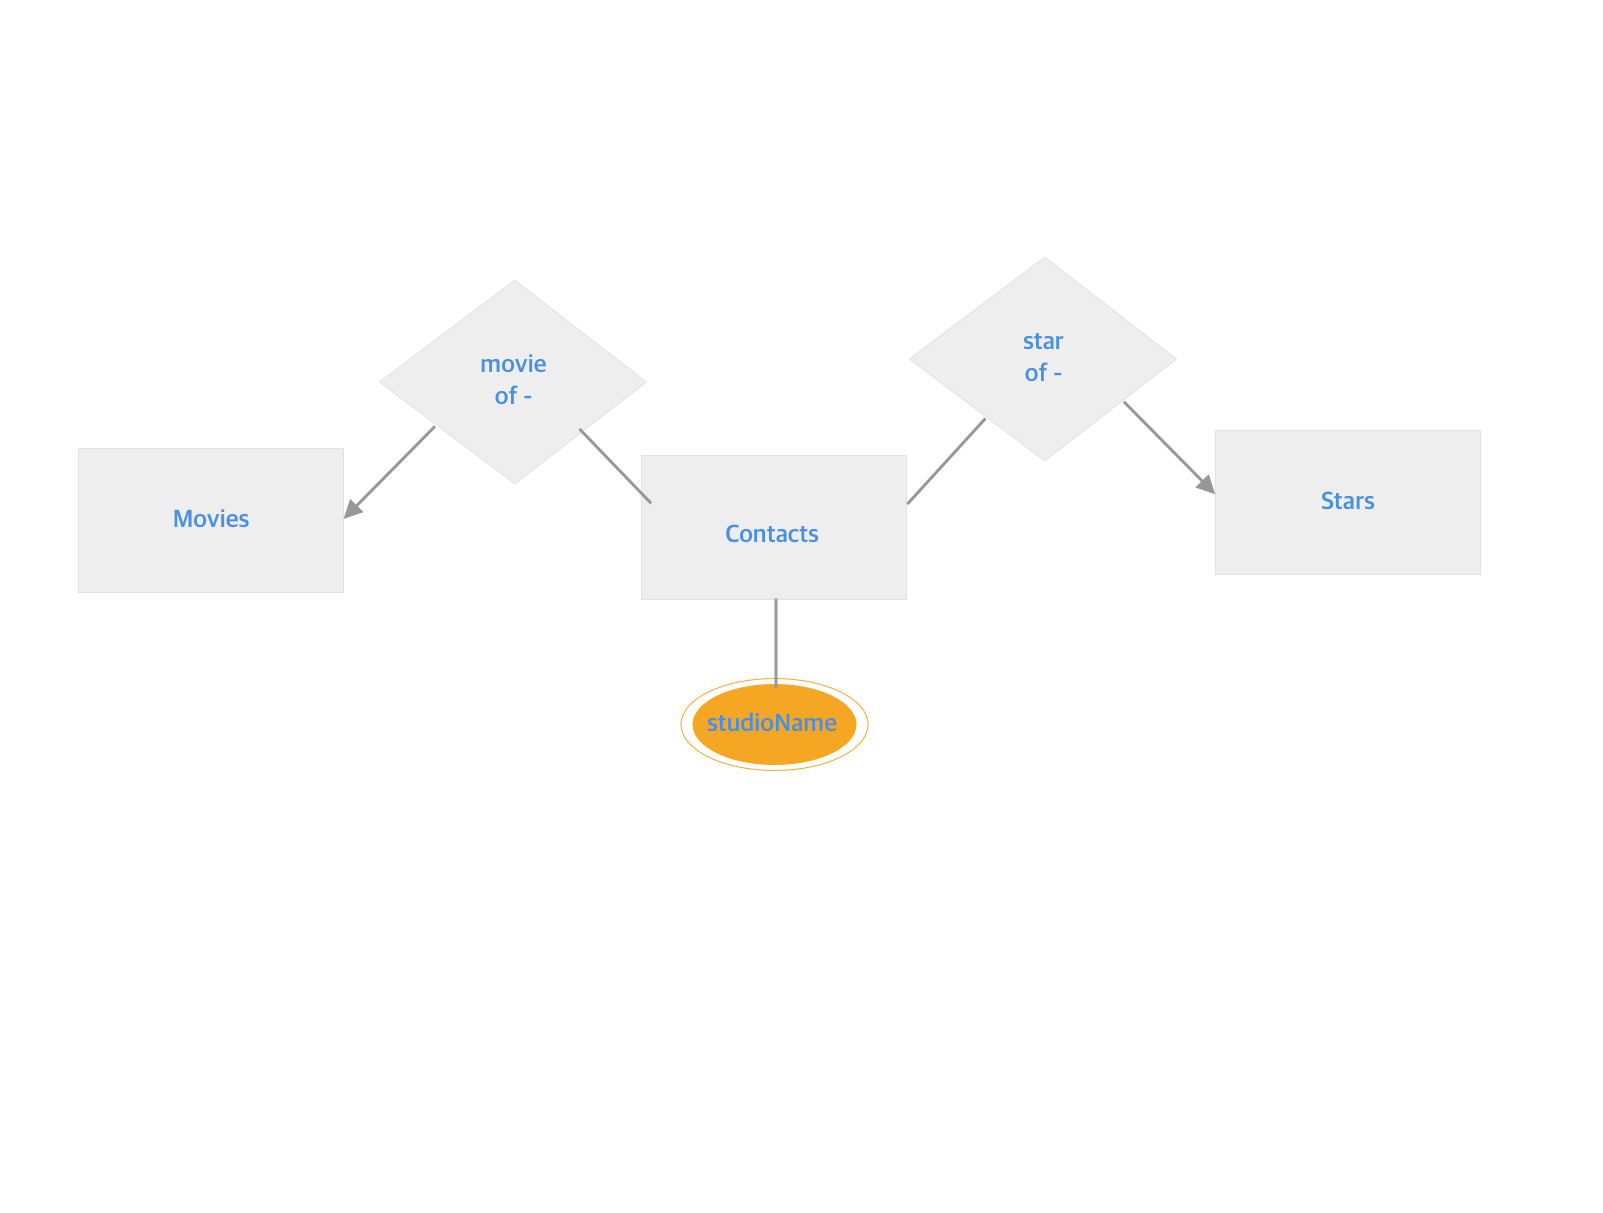
\includegraphics[width=\linewidth]{images/worksheet_14_solution_42.png}
        \end{center}

        \bigskip

        \underline{\textbf{Notes:}}

        \bigskip

        \begin{itemize}
            \item Multivalued attributes is denoted by the following $^{[1]}$

            \begin{center}
            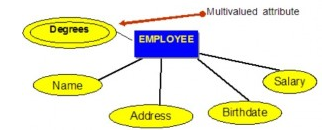
\includegraphics[width=0.7\linewidth]{images/worksheet_14_solution_43.png}
            \end{center}
        \end{itemize}

        \bigskip

        \underline{\textbf{References:}}

        \bigskip

        \begin{enumerate}[1)]
            \item OpenTextBC, The Entity Relationship Model, \href{https://opentextbc.ca/dbdesign01/chapter/chapter-8-entity-relationship-model/}{link}
        \end{enumerate}
    \end{enumerate}

    \item

    \begin{enumerate}[a)]
        \item

        \underline{\textbf{Solution:}}

        \bigskip

        \begin{enumerate}[i)]

            \item

            \begin{center}
            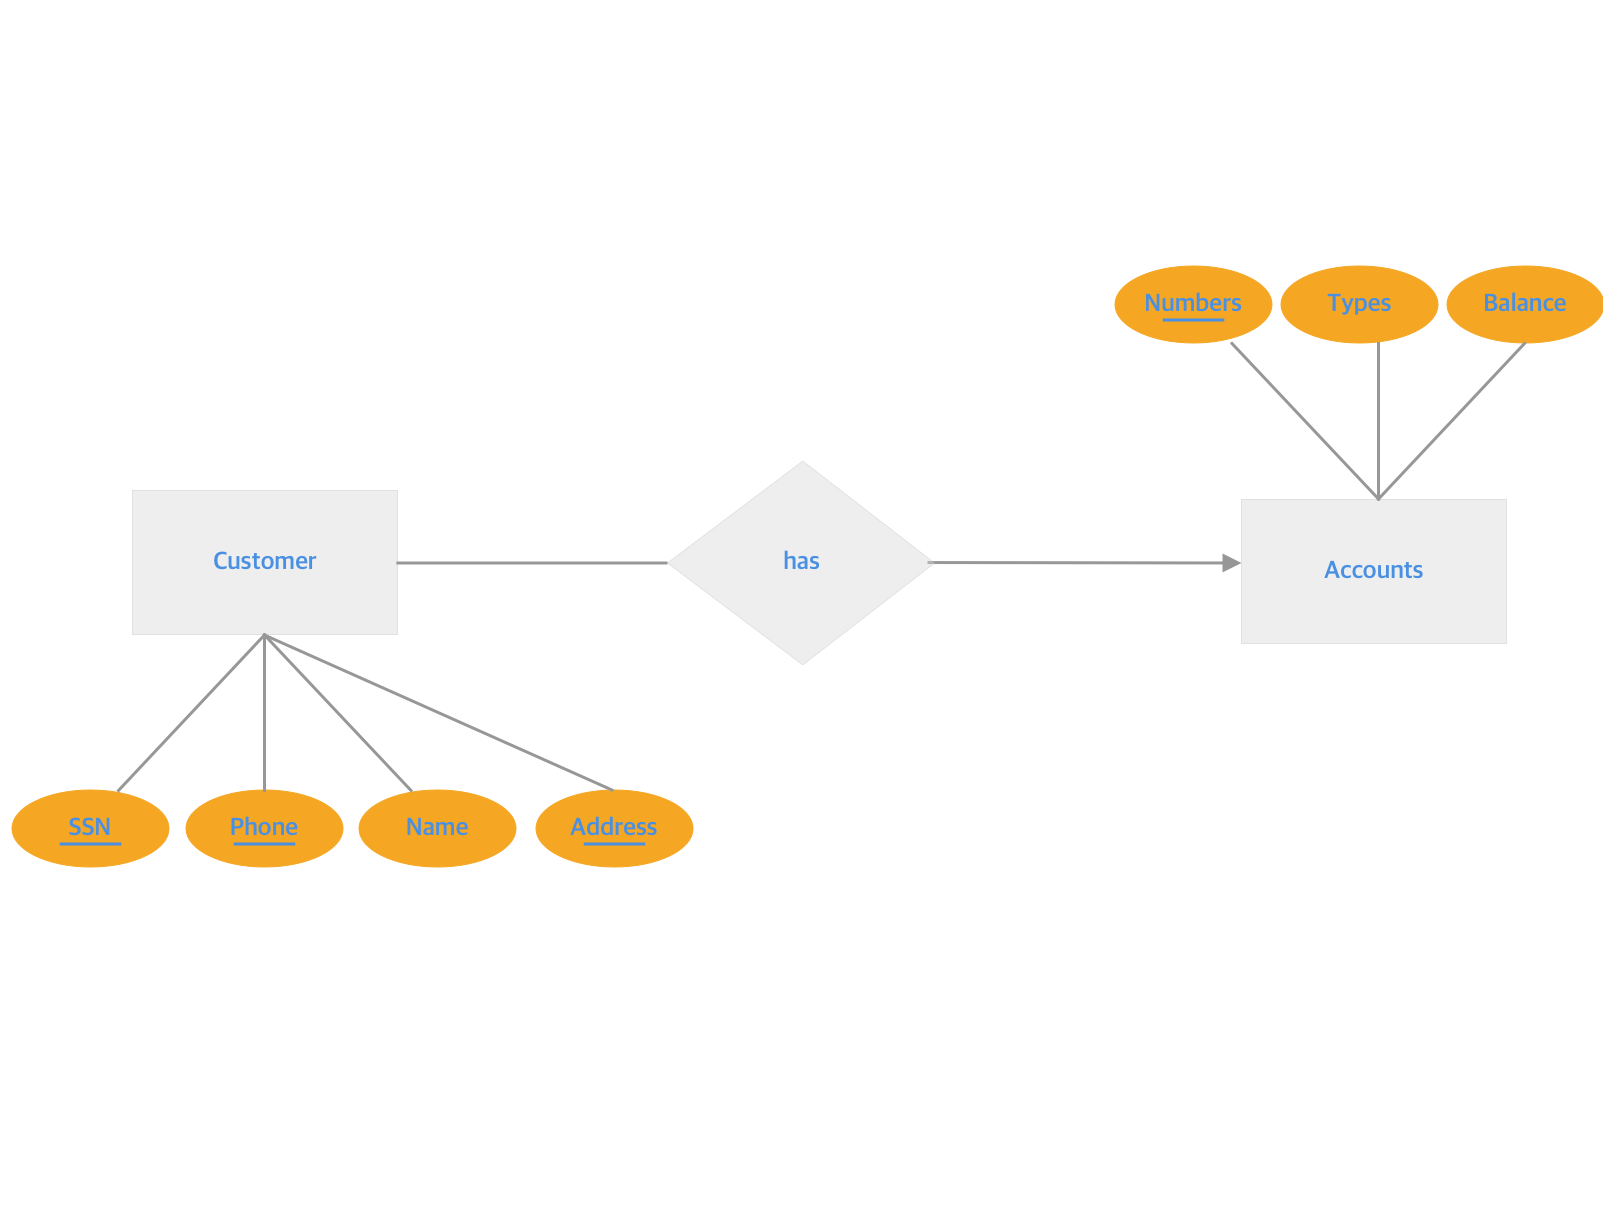
\includegraphics[width=0.7\linewidth]{images/worksheet_14_solution_46.png}
            \end{center}

            \item

            \begin{center}
            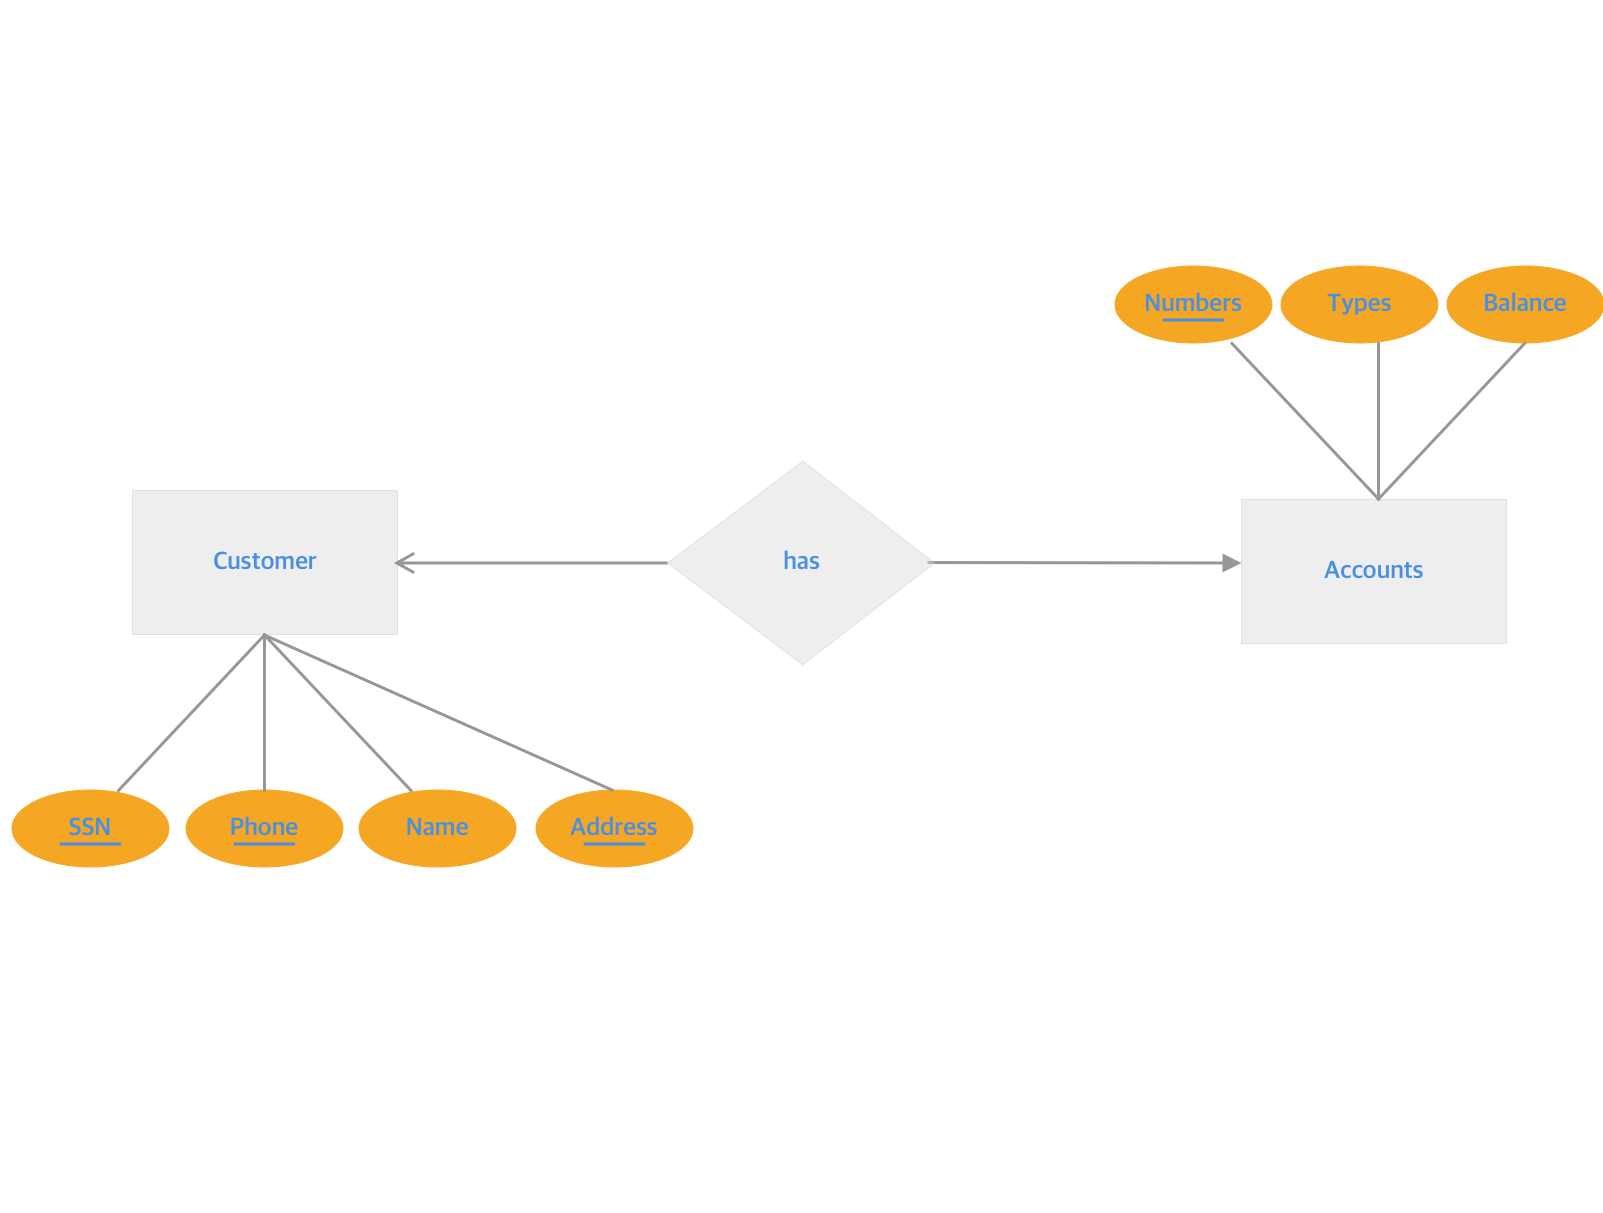
\includegraphics[width=0.7\linewidth]{images/worksheet_14_solution_47.png}
            \end{center}

        \end{enumerate}
        \bigskip

        \underline{\textbf{Notes:}}

        \bigskip

        \begin{itemize}
            \item Keys in the E/R Model

            \begin{itemize}
                \item \textit{key} is an attribute or a group of attributes
                whose values can be used to uniquely identify an individual entity in an
                entity set $^{[1]}$

                \item Keys are represented using `underline' under each attribute

                \begin{center}
                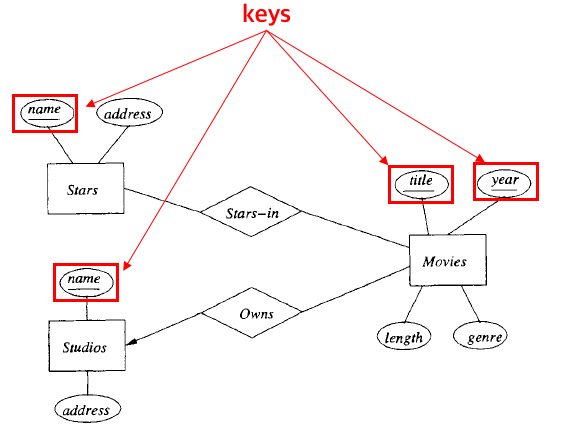
\includegraphics[width=0.7\linewidth]{images/worksheet_14_solution_44.png}
                \end{center}
            \end{itemize}

            \item Referential Integrity

            \begin{itemize}
                \item Means value appearing in one context must also appear in
                another
                \item Functions like Foriegn Key in SQL
                \item Is represented by a rounded arrow

                \begin{center}
                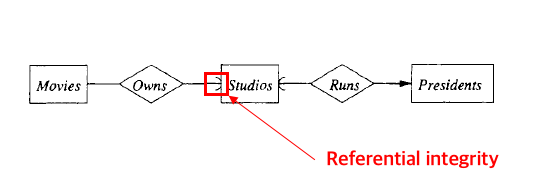
\includegraphics[width=0.7\linewidth]{images/worksheet_14_solution_45.png}
                \end{center}
            \end{itemize}
        \end{itemize}

        \bigskip

        \underline{\textbf{References:}}

        \bigskip

        \begin{enumerate}[1)]
            \item OpenTextBC, The Entity Relationship Model, \href{https://opentextbc.ca/dbdesign01/chapter/chapter-8-entity-relationship-model/}{link}
        \end{enumerate}

        \item

        \underline{\textbf{Solution:}}

        \bigskip

        \begin{enumerate}[i)]

            \item

            \begin{center}
            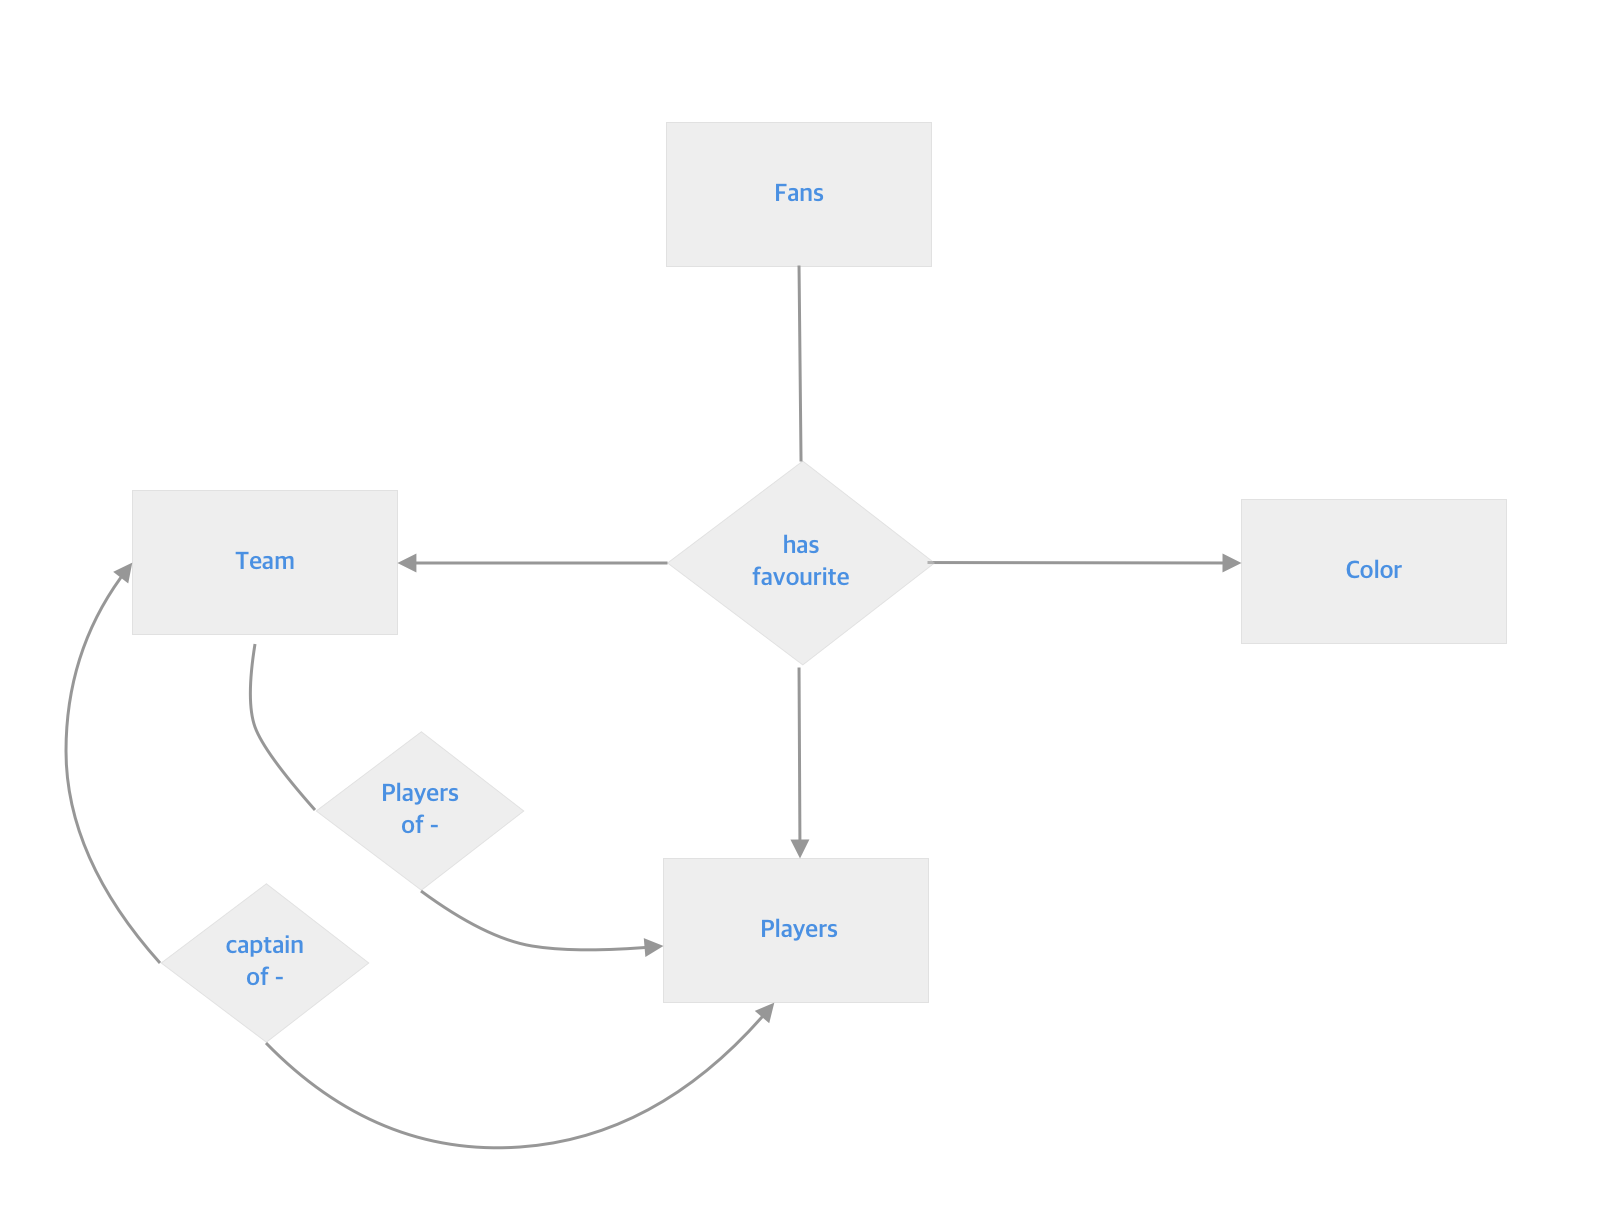
\includegraphics[width=0.7\linewidth]{images/worksheet_14_solution_48.png}
            \end{center}

            \item

            \begin{center}
            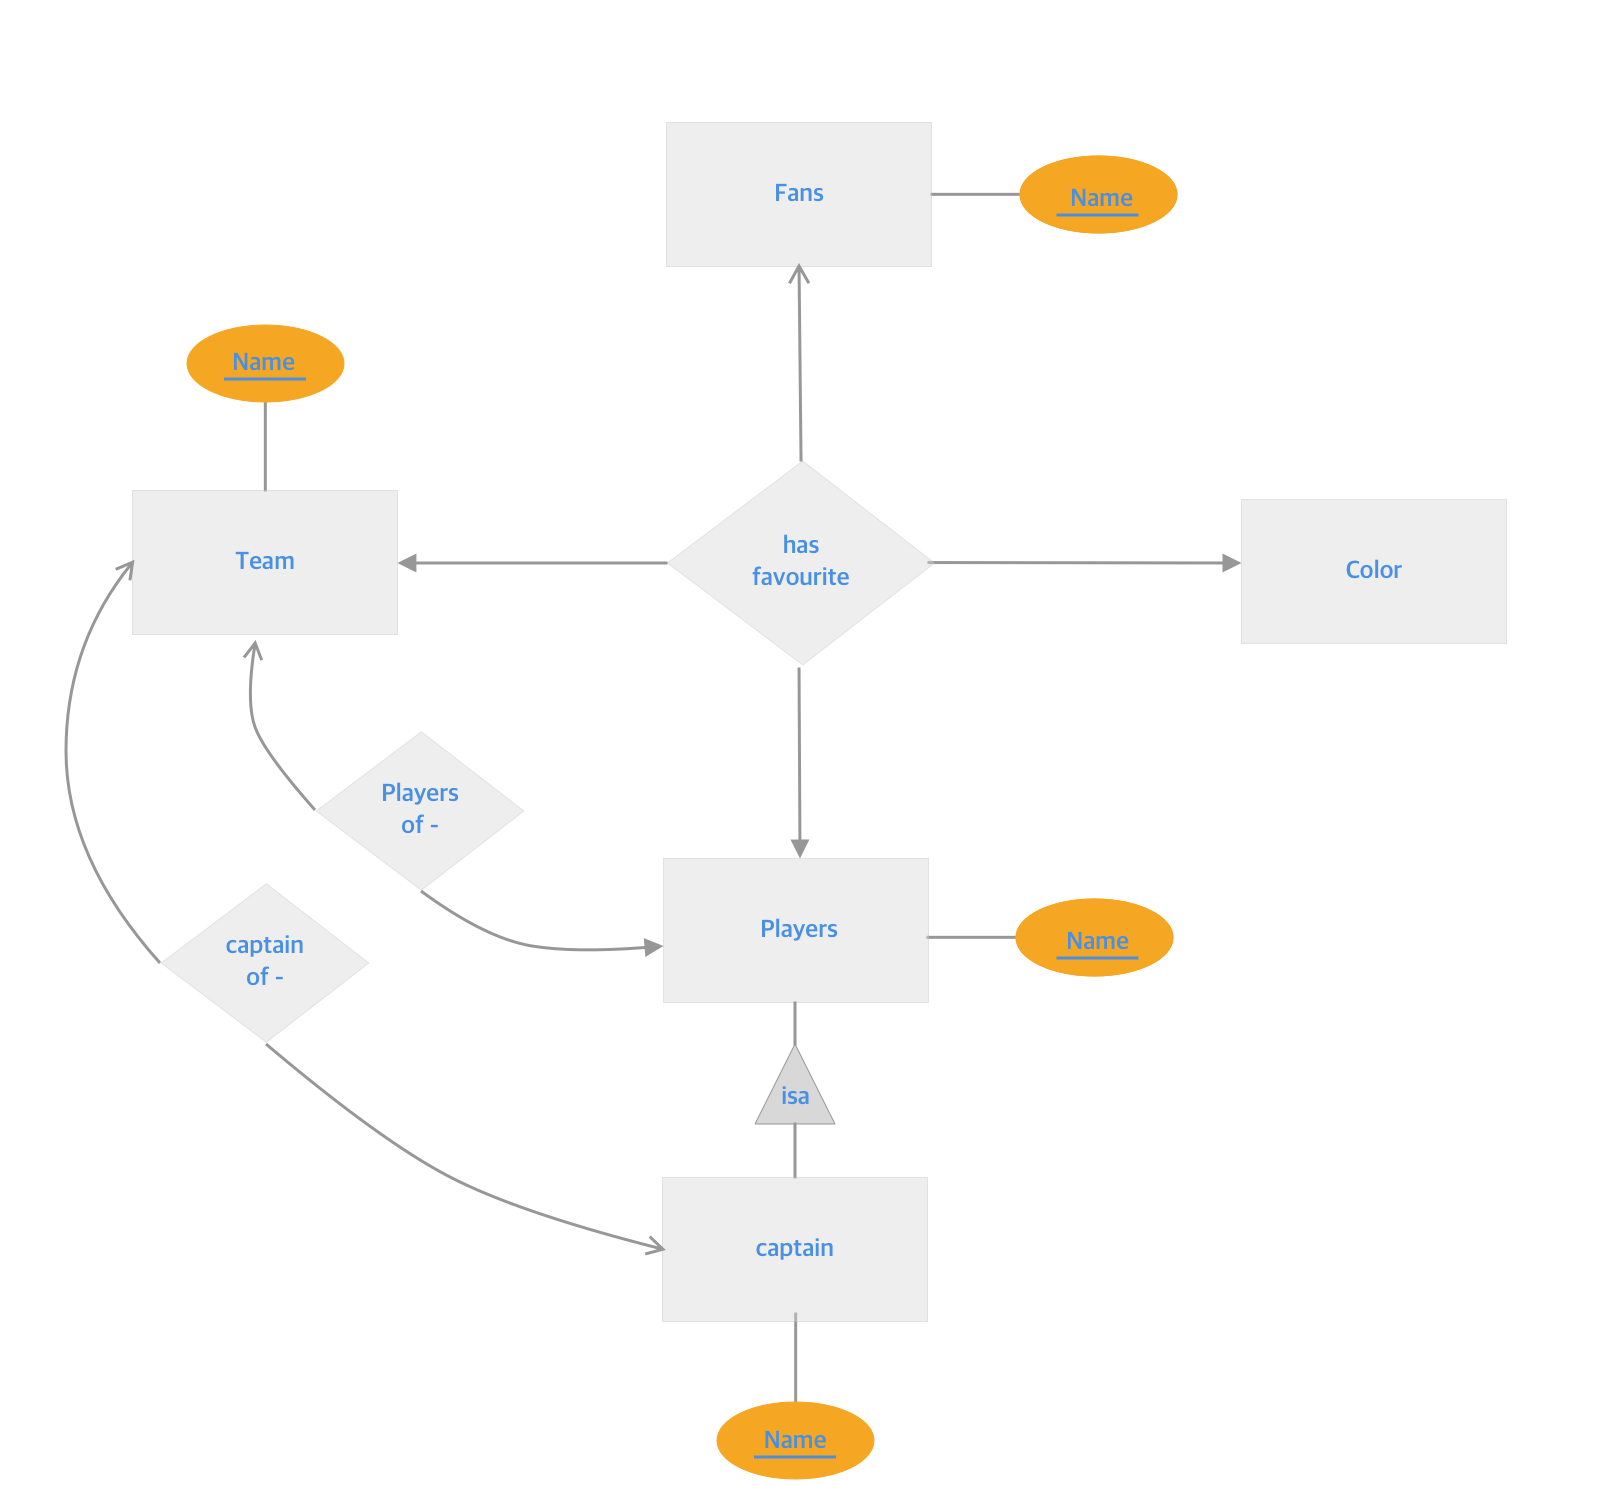
\includegraphics[width=0.7\linewidth]{images/worksheet_14_solution_49.png}
            \end{center}

        \end{enumerate}

        \item

        \underline{\textbf{Solution:}}

        \bigskip

        \begin{enumerate}[i)]

            \item

            \begin{center}
            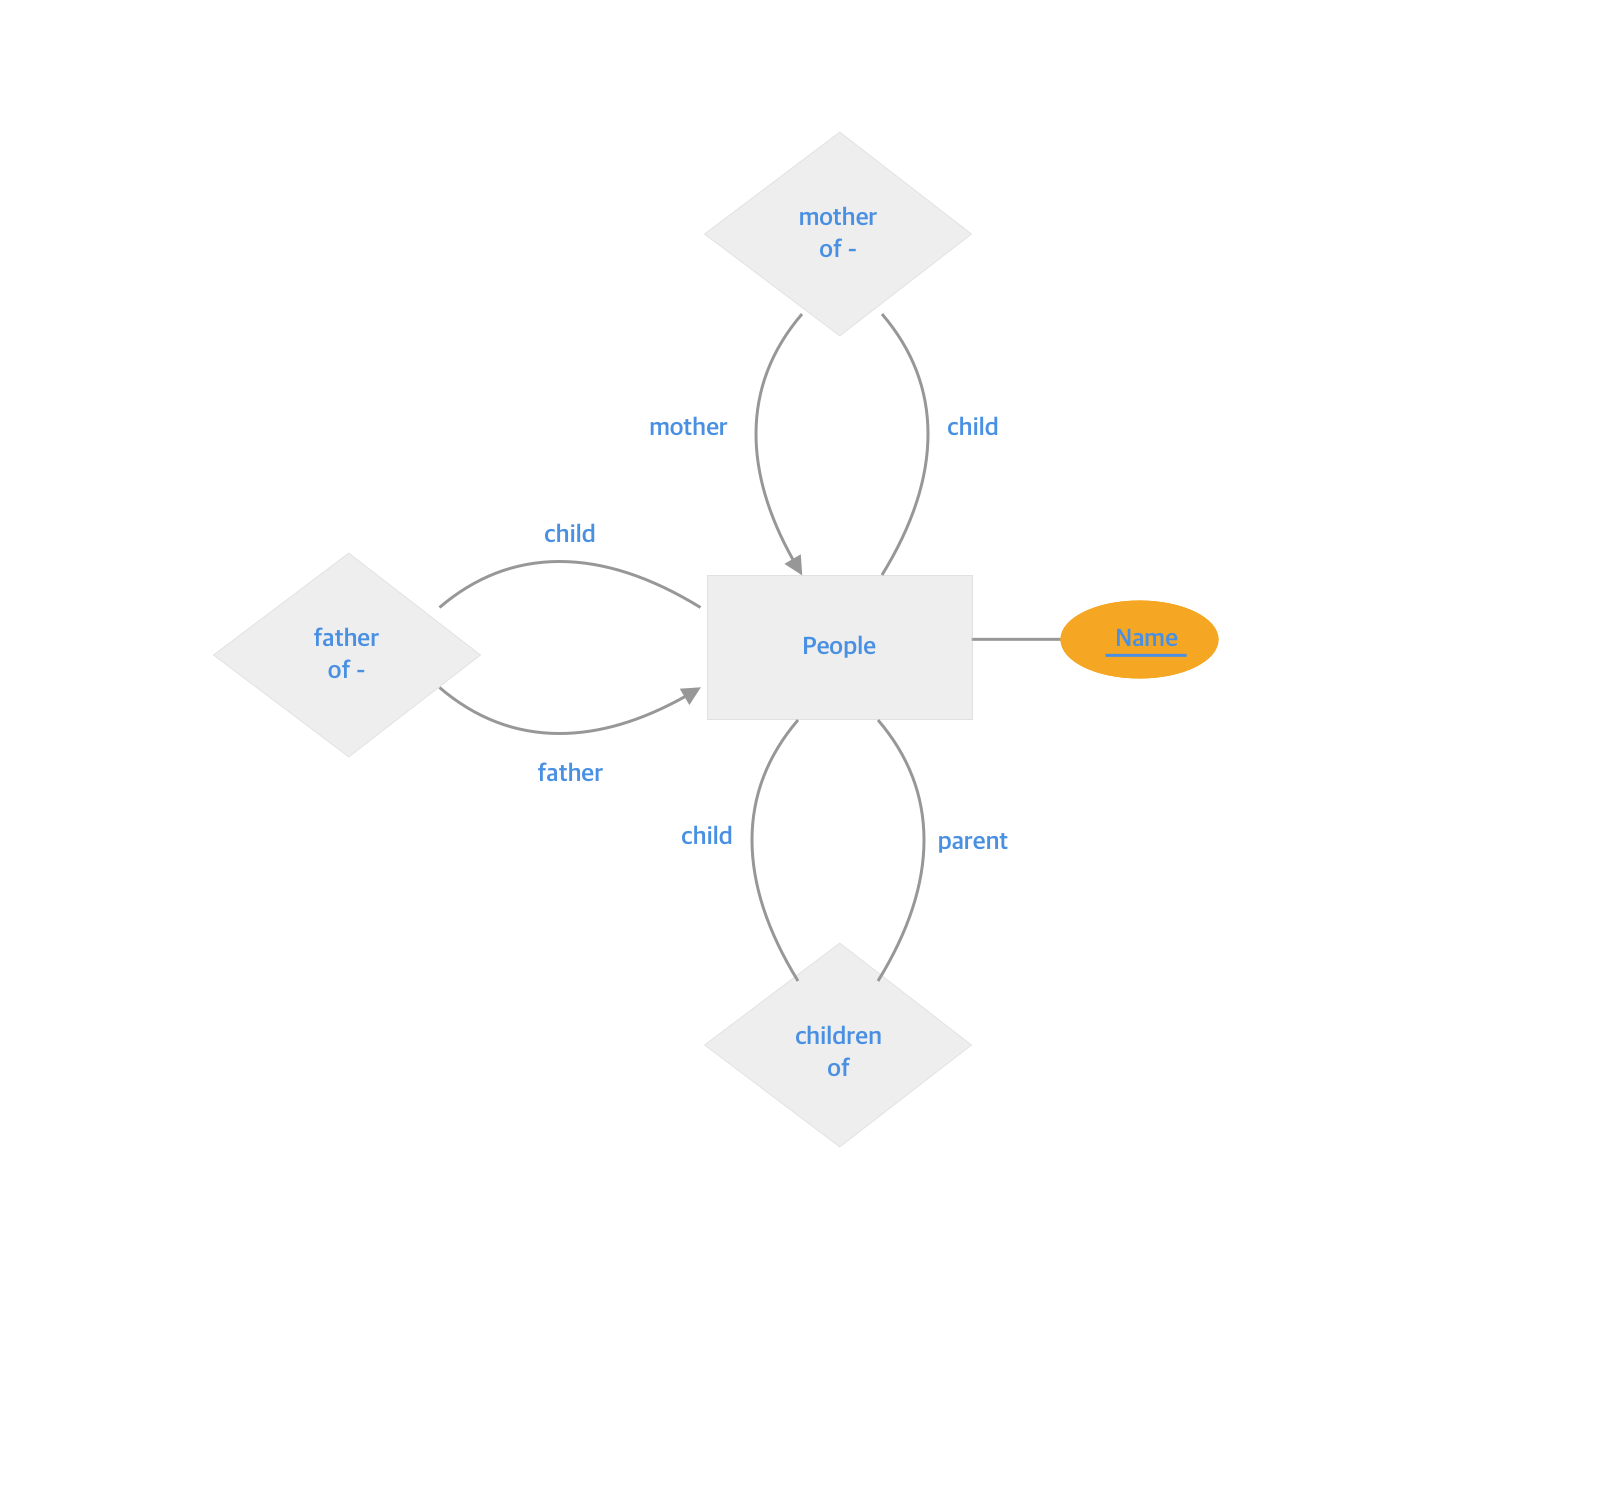
\includegraphics[width=\linewidth]{images/worksheet_14_solution_50.png}
            \end{center}

            \item

            \begin{center}
            \includegraphics[width=\linewidth]{images/worksheet_14_solution_51.png}
            \end{center}


        \end{enumerate}
    \end{enumerate}

    \item

    \underline{\textbf{Solution:}}

    \bigskip

    \begin{center}
    \includegraphics[width=\linewidth]{images/worksheet_14_solution_55.png}
    \end{center}

    \bigskip


    \begin{mdframed}

        \underline{\textbf{Correct Solution:}}

        \bigskip

        \begin{center}
        \includegraphics[width=\linewidth]{images/worksheet_14_solution_57.png}
        \end{center}

        \bigskip

        \color{red}
        \begin{itemize}
            \item Yes. grade is a part of a key for enrollent.
        \end{itemize}
        \color{black}
    \end{mdframed}

    \bigskip

    \underline{\textbf{Notes:}}

    \bigskip

    \begin{itemize}
        \item Weak Entity Sets
        \begin{itemize}
            \item Is an entity set of which some or all of attributes belong to
            another entity set
            \item The usual reason is that there is no global authority capable of creating unique ID’s.
            \item Is denoted by the following symbol:

            \begin{center}
            \includegraphics[width=\linewidth]{images/worksheet_14_solution_52.png}
            \end{center}

            \item Depends on a dominant entity, and it cannot exist without a strong entity. $^{[1]}$
            \item Has attributes in both weak entity sets and the entity sets

            \bigskip

            \underline{\textbf{Example:}}

            \bigskip

            \begin{center}
            \includegraphics[width=\linewidth]{images/worksheet_14_solution_56.png}
            \end{center}

            \bigskip

            \begin{itemize}
                \item Schemas for the strong entity sets

                \begin{itemize}
                    \item student (\underline{username})
                    \item assignment (\underline{shortname}, due\_date, url)
                \end{itemize}

                \item Schemas for the weak entity set

                \begin{itemize}
                    \item submission(\underline{username}, \underline{shortname}, \underline{version}, submit\_date, data)
                \end{itemize}
            \end{itemize}


        \end{itemize}

        \item Requirements for Entity Sets

        \begin{itemize}
            \item E is a weak entity if it consists of

            \begin{enumerate}[1.]
                \item Zero or more of its own attributes, and
                \item One or more many-one relationships to other (supporting) entity sets. $^{[2]}$
            \end{enumerate}

        \end{itemize}

        \begin{center}
        \includegraphics[width=\linewidth]{images/worksheet_14_solution_53.png}
        \includegraphics[width=\linewidth]{images/worksheet_14_solution_54.png}
        \end{center}

    \end{itemize}

    \bigskip

    \underline{\textbf{References:}}

    \bigskip

    \begin{enumerate}[1)]
        \item StackOverflow, Example of a strong and weak entity types, \href{https://stackoverflow.com/questions/4741967/example-of-a-strong-and-weak-entity-types}{link}
        \item Stanford, Entity-Relationship Model, \href{http://infolab.stanford.edu/~ullman/fcdb/aut07/slides/er.pdf}{link}
        \item Caltech, Converting E-R Diagrams to Relational Model, \href{http://users.cms.caltech.edu/~donnie/dbcourse/intro0607/lectures/Lecture17.pdf}{link}
    \end{enumerate}


    \item

    \begin{center}
    \includegraphics[width=\linewidth]{images/worksheet_14_solution_58.png}
    \end{center}

    \item

    \begin{enumerate}[a)]
        \item

        \underline{\textbf{Solution:}}

        \begin{center}
        \includegraphics[width=\linewidth]{images/worksheet_14_solution_59.png}
        \end{center}

        \bigskip

        \begin{mdframed}

            \underline{\textbf{Correct Solution:}}

            \bigskip

            \begin{center}
            \includegraphics[width=\linewidth]{images/worksheet_14_solution_66.png}
            \end{center}

        \end{mdframed}

        \item

        \begin{center}
        \includegraphics[width=\linewidth]{images/worksheet_14_solution_60.png}
        \end{center}

        \bigskip

        \begin{mdframed}

            \underline{\textbf{Correct Solution:}}

            \bigskip

            \begin{center}
            \includegraphics[width=\linewidth]{images/worksheet_14_solution_65.png}
            \end{center}

        \end{mdframed}

        \item

        \begin{center}
        \includegraphics[width=\linewidth]{images/worksheet_14_solution_63.png}
        \end{center}

        \bigskip

        \begin{mdframed}

            \underline{\textbf{Correct Solution:}}

            \bigskip

            \begin{center}
            \includegraphics[width=\linewidth]{images/worksheet_14_solution_64.png}
            \end{center}

        \end{mdframed}

    \end{enumerate}


    \item

    \begin{enumerate}[a)]

        \item

        \underline{\textbf{Solution:}}

        \bigskip

        \begin{center}
        \includegraphics[width=\linewidth]{images/worksheet_14_solution_67.png}
        \end{center}

        \item

        \underline{\textbf{Solution:}}

        \bigskip

        \begin{center}
        \includegraphics[width=\linewidth]{images/worksheet_14_solution_68.png}
        \end{center}

        \bigskip

        \begin{mdframed}

            \underline{\textbf{Correct Solution:}}

            \bigskip

            \begin{center}
            \includegraphics[width=\linewidth]{images/worksheet_14_solution_74.png}
            \end{center}

        \end{mdframed}

    \end{enumerate}

    \item

    \bigskip

    \begin{itemize}
        \item Customers

        \bigskip

        Customer(\underline{SSNo}, number, addr, phone)

        \bigskip

        \item Flights

        \bigskip

        Flights(\underline{number}, day, aircraft)

        \bigskip

        \item Bookings

        \bigskip

        Bookings(\underline{SSNo}, \underline{number}, row, seat)

        \bigskip

        \item toCust

        \bigskip

        toCust (\underline{SSNo}) \color{red}Can be eliminated since subset of Customers\color{black}

        \bigskip

        \item ToFit

        \bigskip

        toFit (\underline{number}) \color{red}Can be eliminated since subset of Flights\color{black}

        \bigskip
    \end{itemize}

    \bigskip

    \underline{\textbf{Notes:}}

    \bigskip

    \begin{itemize}
        \item From entity sets to Relations
        \begin{itemize}
            \item There are two basic steps

            \begin{enumerate}[1.]
                \item Turn each entity set into a relation with the same set of attributes, and
                \item Replace a relationship by a relation whose attributes are the keys for
                the connected entity sets

                \bigskip

                \underline{\textbf{Steps:}}

                \bigskip

                \begin{enumerate}[a.]
                    \item Take key attributes in E and put to the relation of R
                    \item Take attributes of R, and put into its relation

                    \item \color{red}\textbf{Notes:}Don't try to combine entity E with relationship R\color{black}

                    \begin{itemize}
                        \item Doing so can lead to redundancy $\to$ requires normalization
                    \end{itemize}

                    \bigskip

                    \begin{center}
                    \includegraphics[width=\linewidth]{images/worksheet_14_solution_71.png}
                    \end{center}

                \end{enumerate}
            \end{enumerate}

            \item With more difficult steps

            \begin{enumerate}[1.]
                \item Weak entity sets cannot be translated straightforwardly to relation
                \item 'Isa' relationship and subclasses require careful treatment
                \item Sometimes, we do well to combine two relations of different types
                (many-to-one $\to$ many-to-one)
                the connected entity sets
            \end{enumerate}

            \bigskip

            \underline{\textbf{Example:}}

            \bigskip

            \begin{enumerate}[1.]
                \item Turning each entity into relation

                \begin{center}
                \includegraphics[width=\linewidth]{images/worksheet_14_solution_69.png}
                \end{center}

                \item Turning E/R Relationships to Relations

                \begin{itemize}
                    \item The schema of the relation `Owns' is:

                    \begin{align*}
                        Owns(title year, studioName)
                    \end{align*}
                \end{itemize}

                \begin{center}
                \includegraphics[width=\linewidth]{images/worksheet_14_solution_70.png}
                \end{center}
            \end{enumerate}
        \end{itemize}

        \item Handling weak entity sets

        \begin{itemize}
            \item Three things must be done differently

            \begin{enumerate}[1.]
                \item The relation for the weak entity set W must include the
                its own attributes, but also the attributes of the supporting
                entity sets
                \item W should use key of it's attributes in addition to other
                entitity sets that contribute to W's key
                \item \color{red}Do not convert the supporting sets to relation\color{black}
            \end{enumerate}
        \end{itemize}

        \bigskip

        \underline{\textbf{Example:}}

        \bigskip

        \begin{center}
        \includegraphics[width=\linewidth]{images/worksheet_14_solution_72.png}
        \end{center}

    \end{itemize}

    \item

    \begin{enumerate}[a)]
        \item

        \begin{center}
        \includegraphics[width=\linewidth]{images/worksheet_14_solution_73.png}
        \end{center}

        \item

        \begin{itemize}
            \item Bookings (\underline{number}, \underline{day}, row, seat)
            \item Flights (\underline{day}, \underline{nunber}, aircraft)
        \end{itemize}

        \bigskip

        No. It's not the same as the E/R in exercise 5.2.
    \end{enumerate}

    \item

    \begin{itemize}
        \item SisterOf(\underline{shipName}, \underline{sisterName})
        \item Ships(\underline{name}, yearLaunched)
    \end{itemize}

    \item

    \begin{enumerate}[a)]
        \item

        \begin{itemize}
            \item Stars

            \bigskip

            Stars(\underline{name}, addr)

            \bigskip

            \item Studios

            \bigskip

            Studios(\underline{name}, addr)

            \bigskip

            \item Movies

            \bigskip

            Studios(\underline{name}, addr)

            \bigskip

            \item Contracts

            \bigskip

            Contracts(\underline{title}, \underline{year}, length, genre)

            \bigskip

            \item Movies

            \bigskip

            Movies(\underline{title}, \underline{year}, length, genre)

            \bigskip

            \item StarOf

            \bigskip

            StarOf(\underline{name}) \color{red}Can be eliminated. Is a subclass of Stars\color{black}

            \bigskip

            \item StudioOf

            \bigskip

            StudioOf(\underline{name}) \color{red}Can be eliminated. Is a subclass of Studio\color{black}

            \bigskip

            \item StudioOf

            \bigskip

            StudioOf(\underline{title}, \underline{year}) \color{red}Can be eliminated. Is a subclass of Movies\color{black}

            \bigskip
        \end{itemize}
        \item

        \begin{itemize}
            \item Enrollment

            \bigskip

            Enrollment(\underline{grade}, \underline{name})

            \bigskip

            \item Student

            \bigskip

            Student(\underline{grade})

            \bigskip

            \item Course

            \bigskip

            Course(\underline{name})

            \bigskip

            \item studentOf

            \bigskip

            studentOf(\underline{grade}) \color{red}Can be eliminated. Is a subset of Student\color{black}

            \bigskip

            \item courseOf

            \bigskip

            courseOf(\underline{name}) \color{red}Can be eliminated. Is a subset of Course\color{black}

            \bigskip
        \end{itemize}
        \item

        \begin{itemize}
            \item Courses

            \bigskip

            Courses(\underline{number})

            \bigskip

            \item Departments

            \bigskip

            Departments(\underline{name})

            \bigskip

            \item Offers

            \bigskip

            Offers(\underline{number}, \underline{name})

            \bigskip
        \end{itemize}

        \item

        \begin{itemize}
            \item Players

            \bigskip

            Players(\underline{number})

            \item TeamsOf

            \bigskip

            TeamsOf(\underline{name}, \underline{number})

            \bigskip

            \item Teams

            \bigskip

            Teams(\underline{name}, \underline{number})

            \bigskip

            \item LeaguesOf

            \bigskip

            LeaguesOf(\underline{leagueName}, \underline{teamsName}) \color{red}Can be eliminated since it's the subset of Leagure\color{black}

            \item Leagues

            \bigskip

            Leagues(\underline{name}, \underline{teamsName})

            \bigskip

        \end{itemize}

        \bigskip

        \underline{\textbf{Notes:}}

        \begin{itemize}
            \item I should clarify with professor on this question. Something doesn't feel right.
        \end{itemize}
    \end{enumerate}

    \item

    \begin{enumerate}[a)]

        \item

        \begin{itemize}
            \item Depts

            \bigskip

            \quad Depts(\underline{name}, chair)

            \bigskip

            \item GivenBy

            \bigskip

            \quad GivenBy(\underline{deptName}, \underline{CoursesNumber}) \color{red}Can be eliminated since it's the subclass of Courses\color{black}

            \bigskip

            \item Courses

            \bigskip

            \quad Courses(\underline{number}, \underline{deptName}, room)

            \bigskip

            \item Lab Courses

            \bigskip

            \quad LabCourses(\underline{number}, \underline{deptName}, computerAllocation)

            \bigskip

        \end{itemize}

        \bigskip

        \underline{\textbf{Notes:}}

        \bigskip

        \begin{itemize}
            \item Coverting Subclass Structure to Relations (Three different approaches)

            \begin{enumerate}[1.]
                \item \textit{E/R Style Conversion:}
                \item \textit{An Object-Oriented Approach}
                \item \textit{Use Null Values}
            \end{enumerate}
            \item E/R-Style Conversion
            \begin{enumerate}[a)]
                \item Create a relation that includes key attributes from it's parent
                \item From a) include all attributes from its own
            \end{enumerate}

            \bigskip

            \underline{\textbf{Example:}}

            \bigskip

            \begin{center}
            \includegraphics[width=\linewidth]{images/worksheet_14_solution_75.png}
            \end{center}

            \bigskip

            \item An Object-Oriented Approach

            \begin{itemize}
                \item A strategy is to enumerate all the possible subtrees of the hierarchy

                \bigskip

                \underline{\textbf{Example:}}

                \bigskip

                \begin{center}
                \includegraphics[width=0.7\linewidth]{images/worksheet_14_solution_76.png}
                \end{center}


                \begin{enumerate}[1.]
                    \item \textit{Movies} alone

                    \bigskip

                    \quad\textbf{Movies(title, year, length, genre)}

                    \bigskip

                    \item \textit{Movies} and \textit{Cartoons} only

                    \bigskip

                    \quad\textbf{MoviesC(title, year, length, genre)}

                    \bigskip

                    \item \textit{Movies} and \textit{Muder-Mysteries} only

                    \bigskip

                    \quad\textbf{MoviesMM(title, year, length, genre, weapon)}

                    \bigskip

                    \item All three entity-sets

                    \bigskip

                    \quad\textbf{MoviesCMM(title, year, length, genre, weapon)}

                    \bigskip

                    \item Voice for MoviesCMM and MoviesMM

                    \bigskip

                    \quad\textbf{Voices(title, year, starName)}

                    \bigskip

                \end{enumerate}


            \end{itemize}

            \item Use Null values to Combine Relations

            \begin{itemize}
                \item Has all attributes belonging to any entity set in the hierarchy
                \item Use `NULL' in each attribute that is not defined for that entity
            \end{itemize}

            \bigskip

            \underline{\textbf{Example:}}

            \bigskip

            \begin{center}
            \includegraphics[width=\linewidth]{images/worksheet_14_solution_77.png}
            \end{center}
        \end{itemize}

        \item

        \begin{itemize}
            \item Depts

            \bigskip

            \quad Depts(\underline{name}, chair)

            \bigskip

            \item GivenBy

            \bigskip

            \quad GivenBy(\underline{deptName}, \underline{courseNumber}) \color{red}Can be eliminated since it's the subclass of Courses\color{black}

            \bigskip

            \item Courses

            \bigskip

            \quad Courses(\underline{number}, \underline{deptName}, room)

            \bigskip

            \item Lab Courses

            \bigskip

            \quad LabCourses(\underline{number}, \underline{deptName}, room, computerAllocation)

            \bigskip
        \end{itemize}

        \item

        \begin{itemize}
            \item Depts

            \bigskip

            \quad Depts(\underline{name}, chair)

            \bigskip

            \item GivenBy

            \bigskip

            \quad GivenBy(\underline{deptName}, \underline{courseNumber}) \color{red}Can be eliminated since it's the subclass of Courses\color{black}

            \bigskip

            \item Courses

            \bigskip

            \quad Courses(\underline{number}, \underline{deptName}, room, computerAllocation (NULL))

            \bigskip

            \item Lab Courses

            \bigskip

            \quad Courses(\underline{number}, \underline{deptName}, room, computerAllocation)

            \bigskip
        \end{itemize}

    \end{enumerate}

    \item

    \begin{enumerate}[a)]
        \item

        \begin{itemize}
            \item Person

            \bigskip

            \quad Person (\underline{name}, \underline{address})

            \bigskip

            \item Child

            \bigskip

            \quad Child (\underline{name}, \underline{address})

            \bigskip

            \item Father

            \bigskip

            \quad Father(\underline{name}, \underline{address})

            \bigskip

            \item Mother

            \bigskip

            \quad Mother (\underline{name}, \underline{address})

            \bigskip

            \item ChildOf

            \bigskip

            \quad ChildOf(\underline{nameOfPerson}, \underline{addressOfPerson},
                    \underline{nameOfChild}, \underline{addressOfChild})

            \bigskip

            \item FatherOf

            \bigskip

            \quad ChildOf(\underline{nameOfChild}, \underline{addressOfChild},
                    \underline{nameOfFather}, \underline{addressOfFather})

            \bigskip

            \item Married

            \bigskip

            \quad Married(\underline{nameOfHusband}, \underline{nameOfHusband},
                    \underline{nameOfWife}, \underline{addressOfWife})

            \bigskip

            \item MotherOf

            \bigskip

            \quad MotherOf(\underline{nameOfChild}, \underline{nameOfChild},
                    \underline{nameOfMother}, \underline{addressOfMother})

            \bigskip
        \end{itemize}
        \item

        \begin{itemize}
            \item Person

            \bigskip

            \quad Person (\underline{name}, \underline{address})

            \bigskip

            \item Child

            \bigskip

            \quad PersonC (\underline{name}, \underline{address})

            \bigskip

            \item Father

            \bigskip

            \quad PersonF(\underline{name}, \underline{address})

            \bigskip

            \item Mother

            \bigskip

            \quad PersonM (\underline{name}, \underline{address})

            \bigskip

            \item Person-Child-Father

            \bigskip

            \quad PersonCF (\underline{name}, \underline{address})

            \bigskip

            \item Person-Child-Mother

            \bigskip

            \quad PersonCM (\underline{name}, \underline{address})

            \bigskip

            \item Person-Father-Mother

            \bigskip

            \quad PersonFM (\underline{name}, \underline{address})

            \bigskip

            \item Person-Child-Father-Mother

            \bigskip

            \quad PersonCFM (\underline{name}, \underline{address})

            \bigskip

            \item ChildOf (For PersonChild, PersonChildMother, PersonChildFather,\\ PersonChildFatherMother)

            \bigskip

            \quad ChildOf(\underline{nameOfPerson}, \underline{addressOfPerson},
                    \underline{nameOfChild}, \underline{addressOfChild})

            \bigskip

            \item FatherOf (For PersonFather, PersonChild, PersonChildFather, \\ PersonChildFatherMother)

            \bigskip

            \quad ChildOf(\underline{nameOfChild}, \underline{addressOfChild},
                    \underline{nameOfFather}, \underline{addressOfFather})

            \bigskip

            \item Married (For PersonFather, PersonMother, PersonFatherMother, \\ PersonChildFatherMother)

            \bigskip

            \quad Married(\underline{nameOfHusband}, \underline{nameOfHusband},
                    \underline{nameOfWife}, \underline{addressOfWife})

            \bigskip

            \item MotherOf (For PersonMother, PersonChild, PersonChildMother, \\ PersonChildFatherMother)

            \bigskip

            \quad MotherOf(\underline{nameOfChild}, \underline{nameOfChild},
                    \underline{nameOfMother}, \underline{addressOfMother})

            \bigskip
        \end{itemize}

        \item


        \begin{itemize}
            \item Person

            \bigskip

            \quad Person (\underline{name}, \underline{address})

            \bigskip

            \item Child

            \bigskip

            \quad Child (\underline{name}, \underline{address})

            \bigskip

            \item Father

            \bigskip

            \quad Father(\underline{name}, \underline{address})

            \bigskip

            \item Mother

            \bigskip

            \quad Mother (\underline{name}, \underline{address})

            \bigskip

            \item ChildOf

            \bigskip

            \quad ChildOf(\underline{nameOfPerson}, \underline{addressOfPerson},
                    \underline{nameOfChild}, \underline{addressOfChild})

            \bigskip

            \item FatherOf

            \bigskip

            \quad ChildOf(\underline{nameOfChild}, \underline{addressOfChild},
                    \underline{nameOfFather}, \underline{addressOfFather})

            \bigskip

            \item Married

            \bigskip

            \quad Married(\underline{nameOfHusband}, \underline{nameOfHusband},
                    \underline{nameOfWife}, \underline{addressOfWife})

            \bigskip

            \item MotherOf

            \bigskip

            \quad MotherOf(\underline{nameOfChild}, \underline{nameOfChild},
                    \underline{nameOfMother}, \underline{addressOfMother})

            \bigskip
        \end{itemize}
    \end{enumerate}

    \item

    \begin{center}
    \includegraphics[width=\linewidth]{images/worksheet_14_solution_78.png}
    \end{center}

    \begin{enumerate}[a)]
        \item

        \begin{itemize}
            \item People

            \bigskip

            \quad People(\underline{name})

            \bigskip
            \item Female

            \bigskip

            \quad Female(\underline{name})

            \bigskip

            \item Male

            \bigskip

            \quad Male(\underline{name})

            \bigskip

            \item Parent

            \bigskip

            \quad Parent(\underline{name})

            \bigskip

            \item isFather

            \bigskip

            \quad isFather(\underline{maleName}, \underline{femaleName})

            \bigskip

            \item isMother

            \bigskip

            \quad isMother(\underline{femaleName}, \underline{maleName})

            \bigskip
        \end{itemize}

        \item

        \begin{itemize}
            \item People

            \bigskip

            \quad People(\underline{name})

            \bigskip
            \item Female

            \bigskip

            \quad PeopleF(\underline{name})

            \bigskip

            \item Male

            \bigskip

            \quad PeopleM(\underline{name})

            \bigskip

            \item Parent

            \bigskip

            \quad PeopleP(\underline{name})

            \bigskip

            \item People-Female-Male

            \bigskip

            \quad PeopleFM(\underline{name})

            \bigskip

            \item People-Female-Parent

            \bigskip

            \quad PeopleFP(\underline{name})

            \bigskip

            \item People-Male-Parent

            \bigskip

            \quad PeopleMP(\underline{name})

            \bigskip

            \item People-Female-Male-Parent

            \bigskip

            \quad PeopleFMP(\underline{name})

            \bigskip

            \item isFather (For PeopleMale, PeopleParent, PeopleMaleParent,\\ PeopleFemaleMaleParent)

            \bigskip

            \quad isFather(\underline{maleName}, \underline{femaleName})

            \bigskip

            \item isMother (For PeopleFemale, PeopleParent, PeopleFemaleParent,\\ PeopleFemaleMaleParent)

            \bigskip

            \quad isMother(\underline{femaleName}, \underline{maleName})

            \bigskip
        \end{itemize}

        \item

        \begin{itemize}
            \item People, Male, Female, Parent

            \bigskip

            \quad People(\underline{name})

            \bigskip

            \item isFather

            \bigskip

            \quad isFather(\underline{maleName}, \underline{femaleName})

            \bigskip

            \item isMother

            \bigskip

            \quad isMother(\underline{femaleName}, \underline{maleName})

            \bigskip
        \end{itemize}
    \end{enumerate}

    \item

    \begin{enumerate}[a)]
        \item

        \begin{itemize}
            \item Minimum number of entities: $e$ (is because each entity needs to turn into relations)
            \item Maximum number of entities: $e$ (is because each entity needs to turn into relations)
            \item Minimum number of components: $a$
            \item Maximum number of components: $a$
        \end{itemize}

        \item

        \begin{itemize}
            \item Minimum number of entities: $e$ (occurs when entities are stacked on top of each other)

            \begin{center}
            \includegraphics[width=0.7\linewidth]{images/worksheet_14_solution_79.png}
            \end{center}

            \item Maximum number of entities: (is because each entity needs to turn into relations)
            \item Minimum number of components:
            \item Maximum number of components:
        \end{itemize}

        \item
    \end{enumerate}

\end{enumerate}

\end{document}